Los criterios de aceptación \texttt{CA-01}--\texttt{CA-07} (Tabla~\ref{tab:criterios_aceptacion}) operacionalizan la verificación de estos objetivos en la campaña experimental del Capítulo~6.
\documentclass[11pt]{article} % Tamaño de letra 11pt

\usepackage[top=2.5cm, bottom=2.5cm, left=2.5cm, right=2.5cm]{geometry} % Márgenes

\usepackage{setspace}
\setstretch{1.15} % Interlineado 1.15

\usepackage{amsmath}
\usepackage{amsfonts}
\usepackage{amssymb}
\usepackage{mathtools}
\usepackage{physics}
\usepackage{cancel}
\usepackage{graphicx}
\usepackage{float}
\usepackage{subcaption}
\usepackage{capt-of}
\usepackage{svg}
\usepackage{enumitem}
\usepackage{cleveref}
\usepackage{array}
\usepackage{verbatim}
\usepackage{xcolor}   % Para colores en dibujos
\usepackage{tikz}     % Para el dibujo de la barra
\usepackage{pdfpages}  % Para insertar PDFs
\usepackage{booktabs} % Para tablas profesionales
\usepackage{tabularx} % Para tablas con ancho controlado
\usepackage{eurosym}  % Para el símbolo del Euro
\usepackage[style=numeric-comp, sorting=none]{biblatex}
%\usepackage[spanish]{babel}
\addbibresource{bibliografia.bib}

\usepackage{listings}
\usepackage{xcolor}

% Configuración de colores para C++
\definecolor{codegreen}{rgb}{0,0.6,0}
\definecolor{codegray}{rgb}{0.5,0.5,0.5}
\definecolor{codesubtle}{rgb}{0.3,0.4,0.5}

\lstset{
    language=C++,
    basicstyle=\ttfamily\small,
    keywordstyle=\color{blue},
    commentstyle=\color{codegreen},
    numberstyle=\tiny\color{codegray},
    numbers=left,
    numbersep=5pt,
    breaklines=true,
    showstringspaces=false
}

\title{TFM - Mateo Bouchet}
\author{Mateo Bouchet}
\date{February 2026}

\begin{document}

\pagenumbering{gobble} % Oculta numeración
\begin{titlepage}
  \AddToShipoutPictureBG*{%
    \put(0,0){%
      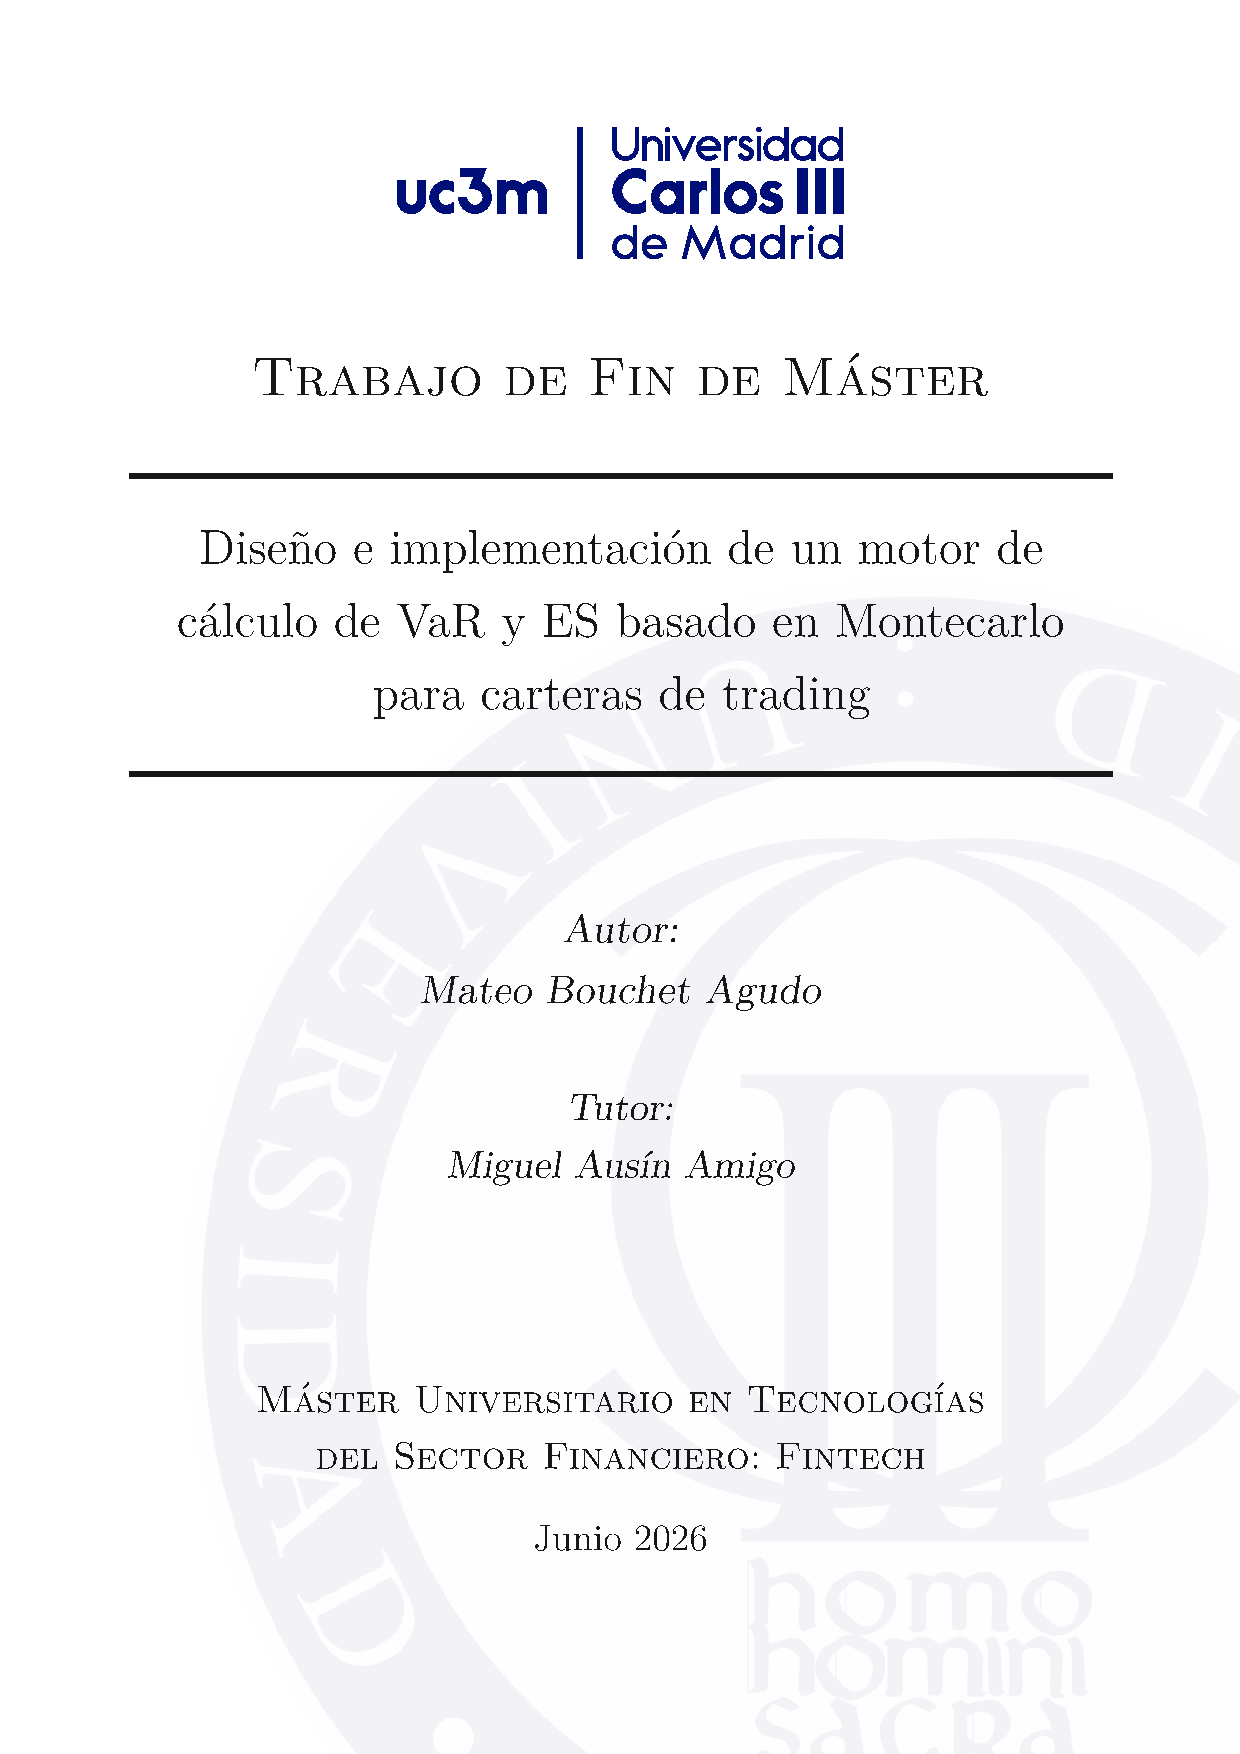
\includegraphics[width=\paperwidth,height=\paperheight]{Fig1.pdf}%
    }%
  }
  \mbox{} % Página vacía con solo el fondo
\end{titlepage}

\clearpage
\pagenumbering{arabic}   % Empieza numeración arábiga
\setcounter{page}{1}     % Desde la página 1
\pagestyle{plain}        % Asegura que los números de página se muestren

\newpage

\begin{center}
  \textbf{Resumen}
\end{center}

\noindent
El cálculo del Value at Risk y del Expected Shortfall sobre carteras diversificadas constituye uno de los principales retos computacionales impuestos por la regulación de riesgo de mercado (marco FRTB).
Frente a alternativas emergentes basadas en aprendizaje automático o computación cuántica---aún limitadas por el riesgo de modelo o la inmadurez del hardware---, este Trabajo de Fin de Máster aborda el problema desde la optimización del método de Monte Carlo clásico: mejorar la precisión estadística de las estimaciones de cola sin sacrificar la auditabilidad del proceso de revaloración.

El objetivo es diseñar, implementar y evaluar un motor modular en C++ capaz de simular escenarios correlacionados, revalorar carteras multi-activo y calcular el \textit{Value at Risk} y el \textit{Expected Shortfall} empíricos sobre la distribución de P\&L.
El sistema integra renta variable (movimiento browniano geométrico), derivados (opciones europeas y de barrera), renta fija con dinámica de tipos Hull--White y una matriz de correlación entre factores de riesgo.
La arquitectura separa el dominio financiero, la orquestación de la simulación y el cálculo de métricas, permitiendo intercambiar generadores aleatorios y parámetros de ejecución sin alterar el núcleo del motor.

La propuesta combina, de forma complementaria, técnicas de reducción de varianza y cuasi-Monte Carlo---Sobol, puentes brownianos y variables antitéticas---con un diseño orientado al alto rendimiento en CPU, manteniendo la revaloración explícita de cada instrumento.

Los resultados empíricos confirman que el cuasi-Monte Carlo mejora la estabilidad de las estimaciones de VaR y ES frente al muestreo pseudoaleatorio a igual número de escenarios, y que los esquemas de error asociados a cada generador permiten cuantificar la incertidumbre de las métricas de cola de manera coherente.
Paralelamente, el análisis de escalado mediante la ley de Amdahl muestra un paralelismo efectivo del motor en la cartera de referencia, a la vez que evidencia cómo el crecimiento del tamaño de la cartera concentra el coste en la revaloración secuencial de activos.

En conjunto, el trabajo demuestra que el Monte Carlo clásico bien diseñado sigue siendo una alternativa madura, auditable y aún mejorable para afrontar las exigencias computacionales del riesgo de mercado contemporáneo.

\newpage

\begin{center}
  \textbf{Abstract}
\end{center}

\noindent
The computation of the \textit{Value at Risk} (VaR) and \textit{Expected Shortfall} (ES) for diversified portfolios represents one of the main computational challenges imposed by modern market risk regulation under the Fundamental Review of the Trading Book (FRTB) framework. In contrast to emerging alternatives based on machine learning or quantum computing---which remain constrained by model risk and hardware immaturity, respectively---this Master's Thesis addresses the problem by optimizing the classical Monte Carlo method, with the objective of improving the statistical accuracy of tail-risk estimates without compromising the auditability of the revaluation process.

The main objective is to design, implement, and evaluate a modular C++ engine capable of generating correlated market scenarios, revaluing multi-asset portfolios, and computing empirical \textit{Value at Risk} and \textit{Expected Shortfall} from the resulting profit-and-loss (P\&L) distribution. The system incorporates equities (modeled through Geometric Brownian Motion), derivatives (European and barrier options), fixed-income instruments under the Hull--White interest rate model, and a correlation matrix linking the underlying risk factors. Its architecture clearly separates the financial domain, the simulation workflow, and the risk-metric computation, allowing random number generators and execution parameters to be exchanged without modifying the core engine.

The proposed approach combines variance reduction and quasi-Monte Carlo techniques---including Sobol sequences, Brownian bridges, and antithetic variates---with a CPU-oriented high-performance implementation that preserves the explicit revaluation of every financial instrument.

The empirical results show that quasi-Monte Carlo provides more stable VaR and ES estimates than conventional pseudo-random sampling for the same number of scenarios. Furthermore, the error estimators associated with each sampling method offer a consistent quantification of the uncertainty inherent in tail-risk metrics. In parallel, a scalability analysis based on Amdahl's Law reveals a high degree of effective parallelism in the reference portfolio while also showing that, as portfolio size increases, the computational cost becomes increasingly dominated by the sequential revaluation of individual assets.

Overall, this work demonstrates that a carefully designed classical Monte Carlo engine remains a mature, auditable, and still highly optimizable solution for meeting the computational demands of contemporary market risk management.

\newpage

\tableofcontents

\newpage

% --- BLOQUE 1: INTRODUCCIÓN Y CONTEXTO ---

% --- BLOQUE 1: INTRODUCCIÓN, ESTADO DE LA CUESTIÓN Y METODOLOGÍA ---

%ASPECTOS IMPORTANTES:
%Comentar que un buen criterio de convergencia es otro punto que favorece la optimización y disminución del número de simulaciones, pero que debido a los fines académicos de este motor, no se implementa (en la mayoría de escenarios, me interesa estudiar cómo trabaja el motor en función del número de simulaciones, por lo que, poder tener esto como parámmetro en lugar de dejárselo al criterio de convergencia da mucho juego para estudiar el comportamiento del motor).

%Creo que en fundamentos teóricos, entraría bien un pequeño apartado que explique los tipos de activos con los que vamos a trabajar (de esta forma, indicamos que hay 3 dimensiones conceptuales diferentes: La parte de mercados, la parte de métricas y algoritmos y la parte de optimización, que eso se evalúa en la rúbrica. Más adelante, debemos seguir trabajando estos 3 frentes)

%Para hacer coincidir el cronograma con el presupuesto, hay que poner 3 meses para los portátiles y licencias, en lugar de 4.

%Tengo que hacer los códigos estos de python para generar resultados comparables

%Unificar notación. Por ejemplo P&L o PnL

%Repasar presupuesto. Estamos usando al final las máquinas o no??

\section{Introducción}

El método de Monte Carlo, formalizado a mediados del siglo XX como una técnica de muestreo estadístico para resolver problemas físicos complejos \cite{metropolis1949monte, ulam1976adventures, segre1970fermi}, encontró su primera aplicación en la ingeniería financiera en 1977 de la mano de Phelim Boyle \cite{boyle1977options}. Boyle demostró que la simulación de múltiples trayectorias aleatorias era la solución idónea para la valoración de opciones cuando los modelos matemáticos cerrados tradicionales, como la fórmula de Black-Scholes, resultaban insuficientes ante la complejidad y las fricciones reales del mercado. 

En la gestión de riesgos contemporánea, esta limitación de los enfoques analíticos tradicionales ya no es un reto aislado, sino un problema estructural. El cálculo de métricas agregadas como el Value at Risk (VaR) \cite{jpmorgan1994riskmetrics} y el Expected Shortfall (ES) \cite{acerbi2002coherence} para carteras de trading modernas exige herramientas capaces de capturar dependencias no lineales y distribuciones de activos con colas pesadas. En este escenario, el método de Monte Carlo se consolida como el estándar de la industria, trasladando el desafío desde el plano puramente analítico hacia una estrategia combinada entre estadística e ingeniería de software de alto rendimiento.

\subsection{Motivación y justificación del proyecto}

La motivación central de este Trabajo de Fin de Máster nace de una desconexión crítica en la práctica financiera actual: la brecha existente entre el prototipado cuantitativo y la implementación eficiente en sistemas de producción. El cálculo del Expected Shortfall sobre carteras diversificadas ---métrica de referencia en el marco FRTB \cite{bcbs2013frtb}--- impone un volumen de revaloración masivo que debe permanecer \emph{auditable}: cada escenario debe poder reconstruirse mediante la revaloración explícita de los instrumentos, sin depender de aproximadores opacos. Frecuentemente, en el entorno académico y de investigación, se prioriza el uso de lenguajes interpretados de alto nivel como Python por su flexibilidad. Sin embargo, estimar el riesgo de cola de una cartera global mediante Monte Carlo requiere re-valorar miles de instrumentos financieros a lo largo de millones de escenarios simulados. Bajo estas condiciones, los costes de abstracción y la gestión automática de memoria de los lenguajes de alto nivel generan cuellos de botella computacionales inasumibles para los presupuestos de cómputo exigidos en la operativa intra-día de una mesa de trading.

Por tanto, este trabajo construye un motor nativo en C++ para estimar VaR y ES con la convicción de que, bajo FRTB, la ingeniería del cómputo pesa tanto como la modelización financiera: no basta acertar en el modelo si el presupuesto de simulaciones o el tiempo por trayectoria vuelven inviable el cálculo.
El riesgo, en ese punto, es saltar demasiado pronto a soluciones que renuncian a reconstruir cada escenario ---metamodelos opacos, aceleradores sin trazabilidad, la conclusión de que el Monte Carlo clásico no escala--- sin comprobar si el coste está en el método o en cómo se implementa por defecto.
Este proyecto toma en serio la segunda posibilidad: usa el motor como instrumento de medición, no como excusa para sustituir el tasador, y la memoria que sigue recoge qué se encontró al hacerlo.

\subsection{Objetivos del proyecto}

Para dar respuesta al desafío técnico y financiero planteado, este proyecto se articula en torno a los siguientes objetivos fundamentales:

\subsubsection{Objetivo General}

Desarrollar e implementar un motor de simulación Monte Carlo en C++ capaz de estimar el riesgo de mercado —mediante VaR y ES— de carteras multiactivo con dependencias entre activos y tipos de interés. Para ello, el proyecto se plantea desde tres frentes que se entrelazan a lo largo del desarrollo: modelizar y valorar por simulación instrumentos heterogéneos, el diseño algorítmico del muestreo y la estimación de riesgo, y la optimización del rendimiento computacional mediante paralelización y ajustes de implementación, validando la precisión estadística de las métricas y la escalabilidad del motor.

\subsubsection{Objetivos Específicos}

\begin{itemize}
    \item Diseñar una arquitectura modular que separe la modelización de activos, la composición de carteras, la generación de aleatorios, la simulación y el cálculo de métricas de riesgo, facilitando la extensión del sistema a nuevos instrumentos o modelos.
    \item Implementar modelos estocásticos para distintos tipos de activo: movimiento browniano geométrico para renta variable, valoración por simulación de opciones europeas y con barrera, y bonos con cupón valorados con dinámica de tipos Hull–White \cite{options2018hull}.
    \item Incorporar correlación entre factores de riesgo, incluyendo la dependencia entre activos y el factor de tipos de interés, mediante una matriz de correlación y su factorización para la generación de shocks correlacionados.
    \item Estimar métricas de riesgo (VaR y ES) a partir de distribuciones empíricas de PnL, con cálculo opcional de errores estándar adaptados al esquema de muestreo empleado (independiente, antitético o por lotes en Sobol).
    \item Comparar distintos generadores de números aleatorios (Mersenne Twister, variables antitéticas y cuasi-Monte Carlo con secuencias de Sobol \cite{matsumoto1998mersenne, hammersley1956new, sobol1967on}) en términos de convergencia de las métricas de riesgo y de coste computacional.
    \item Paralelizar la simulación distribuyendo los lotes de trayectorias entre hilos de ejecución, y analizar la escalabilidad del sistema frente al número de núcleos y al tamaño de la cartera.
    \item Optimizar y caracterizar el rendimiento del motor, evaluando decisiones de implementación como el layout de almacenamiento de matrices, el uso de operaciones vectorizadas (por ejemplo, mediante Eigen/BLAS) y el reparto entre cómputo y acceso a memoria.
    \item Validar el sistema mediante pruebas unitarias, pruebas de integración y experimentos reproducibles sobre una cartera base de referencia, generando resultados comparables para el análisis en la memoria.
\end{itemize}

Más adelante se describen criterios verificables de estos objetivos.

\subsection{Alcance y limitaciones}

\paragraph{Alcance}

El trabajo se circunscribe al diseño e implementación de un motor Monte Carlo para la medición del riesgo de mercado en carteras multiactivo, mediante la estimación de VaR y ES a partir de trayectorias simuladas. El estudio abarca la modelización de instrumentos heterogéneos, la correlación entre factores de riesgo, distintas técnicas de muestreo aleatorio y el análisis de rendimiento del motor en CPU. La validación se realiza mediante experimentos reproducibles sobre carteras de referencia.

\paragraph{Limitaciones}

\begin{itemize}
    \item Datos de mercado reales. Los parámetros de los modelos (volatilidades, correlaciones, curva de tipos, strikes, barreras, etc.) se definen de forma sintética o calibrada de manera simplificada. No se contempla una pipeline completa de calibración histórica ni de mercado en tiempo real.
    \item Universo de instrumentos. El motor no cubre el espectro completo de productos financieros: no incluye, por ejemplo, opciones americanas, derivados de crédito, swaps u otros exóticos. 
    \item Modelización de tipos de interés. Únicamente se emplea el modelo Hull–White de un factor. No se abordan modelos alternativos (CIR, LIBOR market model, modelos multifactoriales más generales) ni el riesgo de crédito o de contraparte.
    \item Supuestos del modelo. Se asume movimiento browniano geométrico para los subyacentes, volatilidades y correlaciones constantes en el horizonte de simulación, y ausencia de saltos, fricciones de mercado, costes de transacción o restricciones de liquidez.
    \item Paralelismo y hardware. La paralelización se limita a memoria compartida en CPU (hilos). No se explora ejecución distribuida, aceleración en GPU ni optimizaciones específicas de despliegue en entornos cloud.
\end{itemize}

\newpage

\section{Fundamentos teóricos y estado del arte en la literatura financiera}

Antes de empezar a hablar de diseño, librerías, optimizaciones... es necesario abrir un paréntesis y comprender las bases de las métricas que vamos a calcular y de los algoritmos que vamos a usar, así como el contexto en el que nos encontramos.

\subsection{Métricas de riesgo: Value at Risk (VaR) y Expected Shortfall (ES)}

La evaluación del riesgo constituye un elemento fundamental en la gestión de carteras y en la medición del desempeño ajustado al riesgo. Entre las medidas más utilizadas tanto en el ámbito académico como profesional destacan el VaR \cite{jpmorgan1994riskmetrics} y el ES \cite{acerbi2002coherence}, dos métricas diseñadas para cuantificar las pérdidas potenciales asociadas a una inversión.

El Value at Risk estima la pérdida máxima esperada de una cartera para un horizonte temporal y un nivel de confianza determinados. Formalmente, si $L$ representa la distribución de pérdidas de una cartera y $\alpha$ el nivel de confianza, el VaR se define como el cuantil $\alpha$ de dicha distribución:

\begin{equation}
VaR_{\alpha}(L)=\inf\{l\in\mathbb{R}:P(L\leq l)\geq\alpha\}.
\end{equation}

De este modo, un VaR al 95\% de 1 millón de euros implica que existe una probabilidad del 95\% de que las pérdidas no superen dicha cantidad durante el horizonte temporal considerado. Esta medida se ha convertido en un estándar de la industria financiera debido a su interpretación intuitiva y a su facilidad de implementación mediante métodos paramétricos, simulación histórica o simulación de Monte Carlo.

Sin embargo, el VaR presenta una limitación importante: no proporciona información sobre la magnitud de las pérdidas cuando estas superan el umbral estimado. En otras palabras, identifica el punto a partir del cual se sitúan los escenarios más adversos, pero no informa acerca de la severidad de dichos escenarios. Para solventar esta deficiencia se emplea el \textit{Expected Shortfall} (ES), también conocido como \textit{Conditional Value at Risk} (CVaR).

El Expected Shortfall mide la pérdida media esperada condicionada a que esta sea superior al VaR correspondiente. Matemáticamente, puede expresarse como:

\begin{equation}
ES_{\alpha}(L)=E[L \mid L>VaR_{\alpha}(L)].
\end{equation}

La Figura \ref{fig:var_es} ilustra la diferencia conceptual entre ambas métricas sobre una distribución de pérdidas y ganancias (P\&L) con cola pesada. Mientras que el VaR identifica el umbral a partir del cual se sitúan los peores escenarios, el ES considera la pérdida media dentro de dicha región extrema. Como puede observarse, la presencia de eventos de baja probabilidad pero elevado impacto provoca que el ES se sitúe más alejado del centro de la distribución que el VaR, reflejando una mayor sensibilidad al riesgo de cola.

\begin{figure}[H]
    \centering
    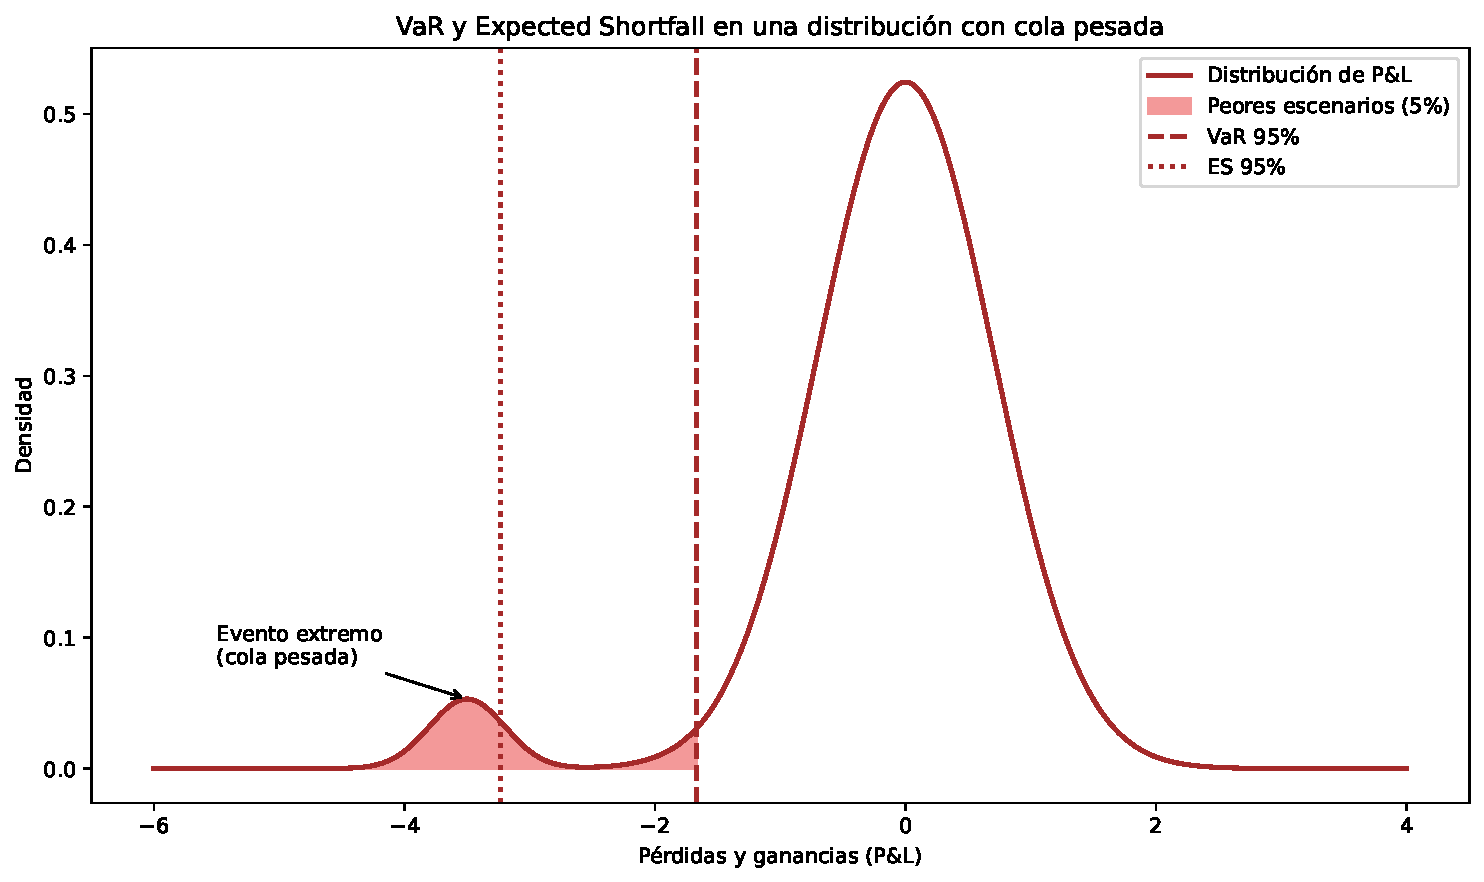
\includegraphics[width=0.8\textwidth]{Fig2.pdf}
    \caption{Representación del Valor en Riesgo (VaR) y del Expected Shortfall (ES) sobre una distribución de pérdidas y ganancias (P\&L) con cola pesada. El VaR delimita el umbral correspondiente al 5\% de los peores escenarios, mientras que el ES mide la pérdida media condicionada a superar dicho umbral.}
    \label{fig:var_es}
\end{figure}

Por tanto, mientras que el VaR establece un umbral de pérdidas, el ES cuantifica la pérdida promedio dentro de la cola de la distribución, proporcionando una visión más completa del riesgo extremo. Por ejemplo, si una cartera presenta un VaR al 95\% de 1 millón de euros y un ES al 95\% de 1,5 millones, ello significa que, en el 5\% de los peores escenarios, la pérdida media esperada asciende a 1,5 millones de euros.

Desde un punto de vista teórico, el Expected Shortfall posee además propiedades matemáticas deseables que el VaR no siempre cumple, como la subaditividad, lo que permite considerarlo una medida de riesgo coherente \cite{artzner1999coherent}. Por esta razón, en los últimos años ha adquirido una importancia creciente en la regulación financiera internacional y ha sustituido progresivamente al VaR como referencia principal para la medición del riesgo de mercado en los marcos regulatorios más recientes \cite{bcbs2013frtb}.

En consecuencia, ambas métricas deben entenderse como herramientas complementarias. El VaR proporciona una estimación sencilla e intuitiva del nivel de pérdidas que puede alcanzarse con una determinada probabilidad, mientras que el ES permite evaluar la gravedad de las pérdidas en los escenarios más desfavorables. La utilización conjunta de ambas medidas ofrece una caracterización más completa del perfil de riesgo de una cartera y resulta especialmente útil en contextos donde la presencia de eventos extremos puede afectar significativamente a los resultados de inversión.

\subsection{Simulación de Monte Carlo}

Para comprender por qué la industria financiera destina tantos recursos computacionales a ejecutar simulaciones de Monte Carlo, es necesario entender su principio fundamental: resolver problemas complejos mediante el uso de la aleatoriedad.

La intuición detrás del método se entiende a la perfección si nos planteamos la siguiente pregunta de ejemplo: ¿Cuál es la probabilidad exacta de ganar una partida de solitario con una baraja estándar de 52 cartas?

Intentar responder a esto mediante fórmulas matemáticas tradicionales es casi imposible debido al enorme número de combinaciones potenciales de las cartas y a la naturaleza no lineal de las reglas del juego. Sin embargo, el método de Monte Carlo propone una alternativa mucho más sencilla: si jugamos $100$ partidas completas registrando cuántas de ellas ganamos, la frecuencia relativa obtenida nos ofrecerá una estimación directa de la probabilidad de victoria sin necesidad de resolver ninguna fórmula sobre el papel.

Este muestreo empírico permite resolver también problemas matemáticos abstractos como la estimación del número $\pi$. 

Imaginemos un cuadrado de lado $2$ (con un área total de $4$) que encierra perfectamente a un círculo de radio $1$ (con un área de $\pi$) como se muestra en la Figura \ref{fig:pi_montecarlo} (a). Si lanzamos un dardo de forma completamente aleatoria sobre el cuadrado, la probabilidad de que impacte dentro del círculo viene determinada por la proporción entre ambas áreas, es decir, $\pi/4$. 

Si disparamos un número masivo $N$ de dardos independientes y contamos cuántos de ellos ($N_{\text{dentro}}$) caen dentro de la diana (como se muestra en la Figura \ref{fig:pi_montecarlo} (b)), la proporción de aciertos se convierte en nuestro estimador muestral:

\begin{equation}
\frac{N_{\text{dentro}}}{N} \approx \frac{\pi}{4}
\end{equation}

\begin{figure}[H]
    \centering
    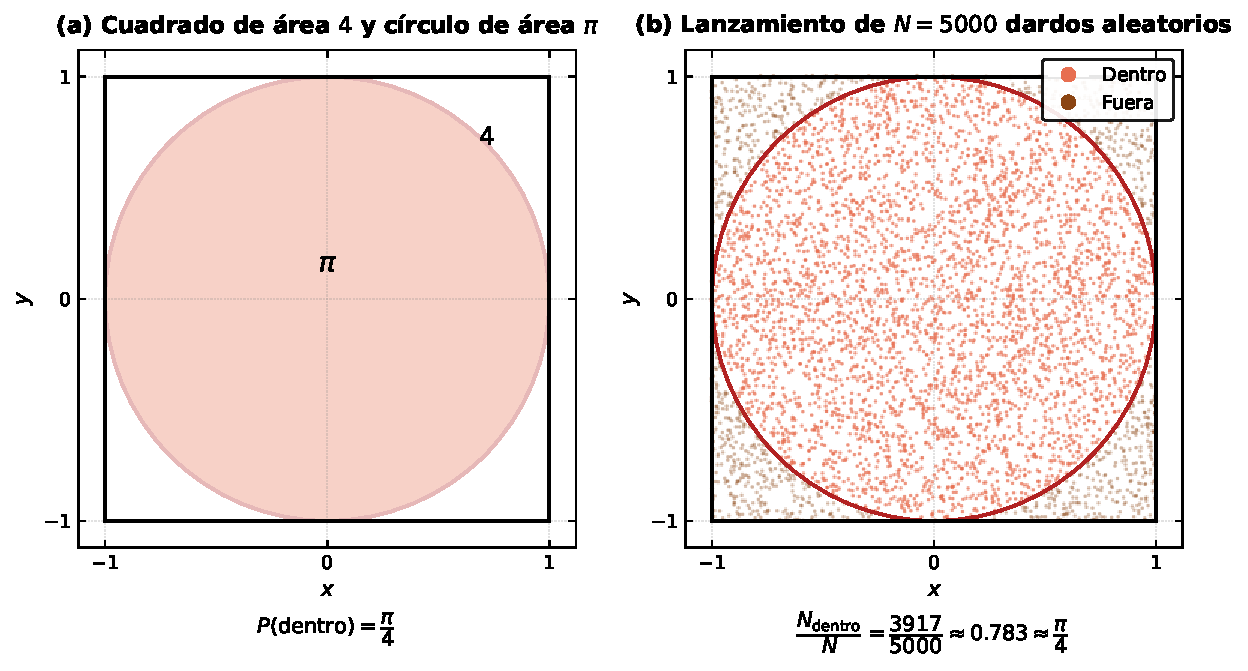
\includegraphics[width=0.8\textwidth]{Fig3.pdf}
    \caption{Estimación de $\pi$ por Monte Carlo mediante el método del dardo. (a) Cuadrado de lado 2 (área 4) con un círculo inscrito de radio 1 (área $\pi$); la probabilidad de que un punto uniforme caiga dentro del círculo es $P(dentro) = \pi/4$. (b) Simulación con $N = 5000$ lanzamientos independientes y uniformes sobre el cuadrado; los puntos dentro del círculo ($N_{\text{dentro}} = 3917$) permiten estimar la proporción $N_{\text{dentro}}/N \approx 0,783 \approx \pi/4$.}
    \label{fig:pi_montecarlo}
\end{figure}

Despejando de la ecuación anterior, el valor de $\pi$ se puede aproximar de forma puramente numérica multiplicando dicha proporción por cuatro:

\begin{equation}
\pi \approx 4 \times \frac{N_{\text{dentro}}}{N}
\end{equation}

Este experimento demuestra la verdadera esencia del método de Monte Carlo: transformar un problema de cálculo continuo analítico (generalmente complejo) en un problema de conteo estadístico discreto (computacionalmente abordable). 

\subsubsection{Formalismo para cálculo de VaR y ES con Monte Carlo}

En el mundo de la gestión de riesgos, el ``área'' multidimensional que se pretende medir ya no es un círculo plano, sino la distribución de pérdidas y ganancias (P\&L) de una cartera de trading en un horizonte temporal futuro $T$ (por ejemplo, a 1 día o 10 días vista). 

Matemáticamente, si la cartera está compuesta por $d$ activos financieros correlacionados entre sí y expuestos a factores dinámicos como las curvas de tipos de interés modelizadas mediante el proceso de Hull-White \cite{hull1990pricing}, su estado futuro dependerá de un vector multidimensional $\mathbf{S}_T = (S_T^1, S_T^2, \dots, S_T^d)^T$, donde cada componente $S_T^j$ representa explícitamente el precio o valor del activo $j$ en el horizonte temporal $T$. El valor final de la cartera viene determinado por una función de impacto financiero o modelo de valoración de mercado $V_T = f(\mathbf{S}_T)$, de modo que la ganancia o pérdida neta se define como $\Delta V = V_T - V_0$, siendo $V_0$ el valor inicial y conocido de la cartera.

Para calcular de forma exacta el riesgo de esta cartera, la estadística exige resolver una integral multidimensional sobre el espacio de la función de densidad de probabilidad conjunta de todos los precios de los activos del mercado, denotada por $p(\mathbf{S}_T)$:

\begin{equation}
\mathbb{E}[g(\Delta V)] = \int_{\mathbb{R}^d} g(f(\mathbf{S}_T) - V_0) \, p(\mathbf{S}_T) \, d\mathbf{S}_T
\end{equation}
donde $g(\cdot)$ representa la función de transformación asociada a la métrica que se desea obtener, como las funciones indicadoras necesarias para extraer el VaR o el ES. 

El problema crítico es que, cuando el número de activos ($d$) crece o los contratos presentan pagos fuertemente no lineales, esta integral se vuelve matemáticamente intratable. Los métodos de integración numérica tradicionales presentan un coste computacional que escala de forma exponencial por cada nueva dimensión (activo) que se añade al problema. Esta limitación hace inviable su cálculo dentro de las ventanas temporales exigidas en una sala de negociación real.

El método de Monte Carlo rompe esta barrera aplicando exactamente la misma lógica probabilística que en el cálculo de $\pi$. En lugar de intentar resolver la geometría de la integral analítica mediante una cuadrícula rígida de puntos, el motor de riesgo genera $N$ escenarios o caminos aleatorios futuros para los precios de los activos, $\{\mathbf{S}_T^{(i)}\}_{i=1}^N$, respetando su estructura de correlación lineal como se muestra en la Fig. \ref{fig:montecarlo_sim}.

\begin{figure}[htbp]
    \centering
    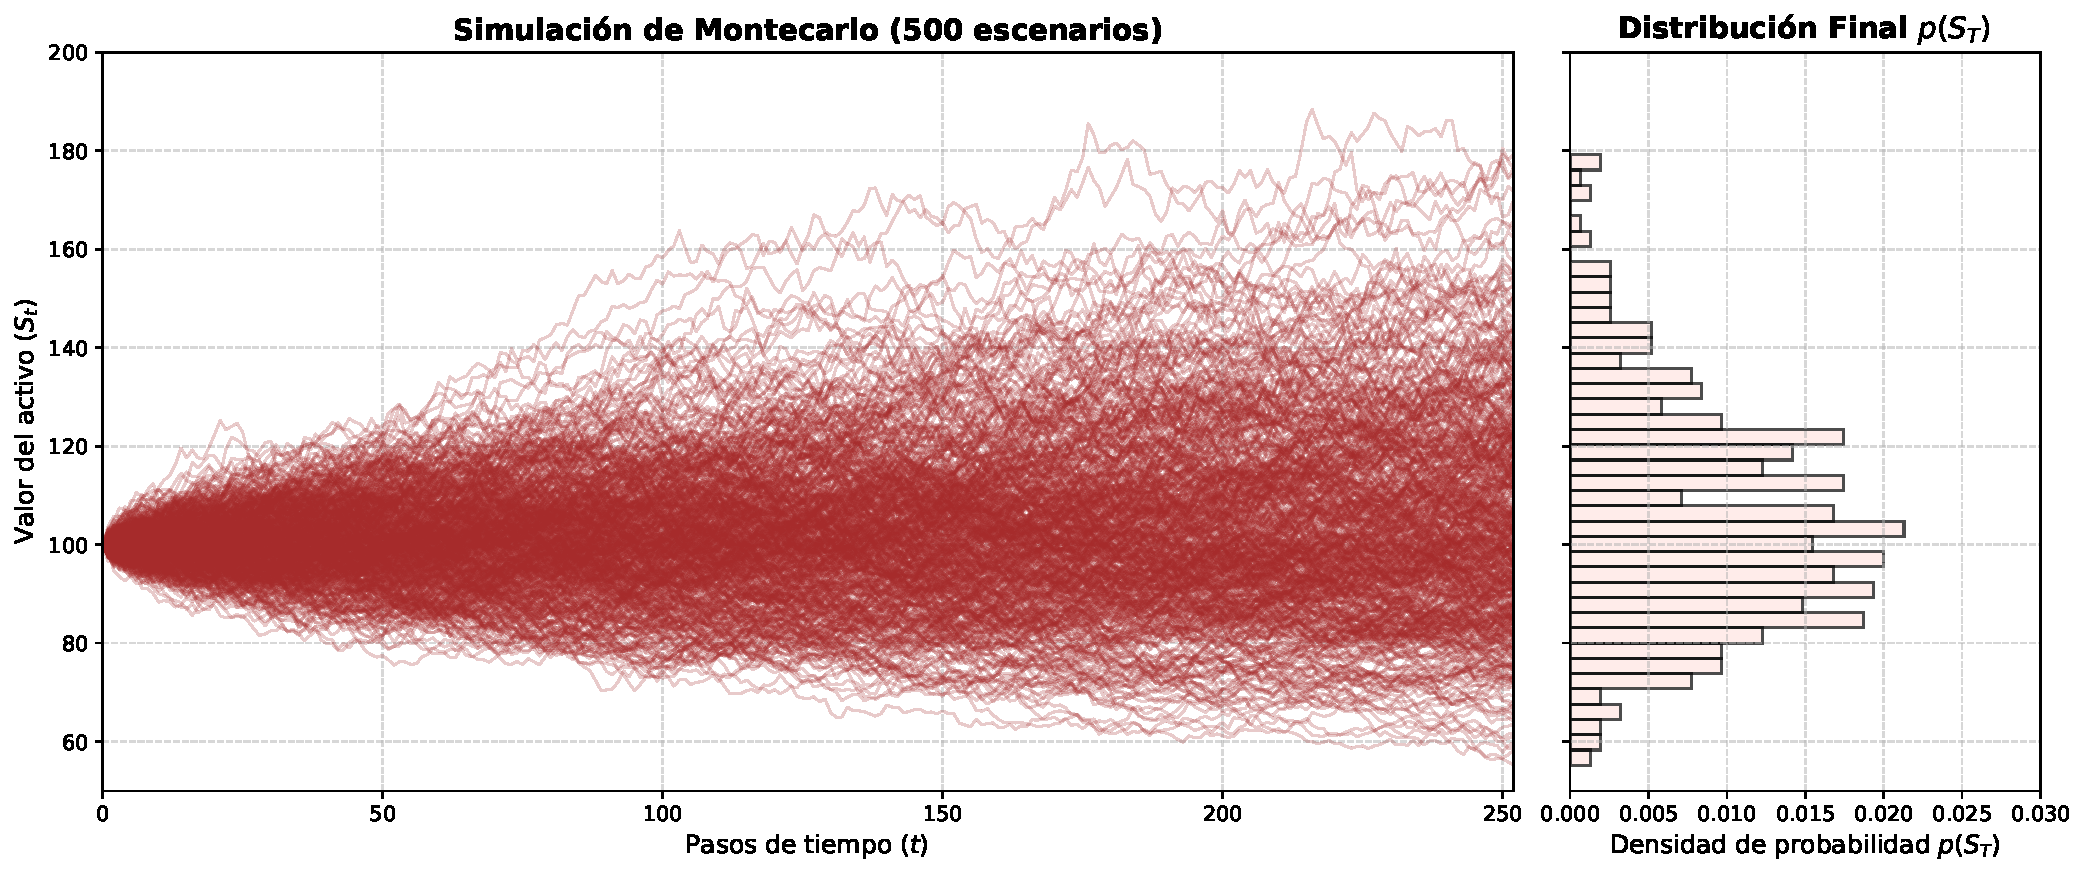
\includegraphics[width=1\textwidth]{Fig4.pdf}
    \caption{Evolución temporal del precio de un activo (panel izquierdo) y su correspondiente distribución de probabilidad al final del periodo simulado (panel derecho).}
    \label{fig:montecarlo_sim}
\end{figure}

Al evaluar el P\&L de la cartera en cada uno de esos $N$ escenarios de precios simulados, se sustituye la integral exacta por una aproximación directa basada en la media aritmética muestral:

\begin{equation}
\mathbb{E}[g(\Delta V)] \approx \frac{1}{N} \sum_{i=1}^{N} g(f(\mathbf{S}_T^{(i)}) - V_0)
\end{equation}

La propiedad fundamental de este enfoque es que, la velocidad de convergencia es completamente independiente del número de activos $d$ que componen la cartera, de tal forma que el método permite evaluar riesgos en carteras de alta dimensionalidad con un coste computacional viable.

\subsubsection{Justificación estadística y el cuello de botella del método}

Esta aproximación numérica es estadísticamente robusta gracias a los dos pilares que sustentan el comportamiento de los promedios aleatorios en la teoría de la probabilidad:

\begin{itemize}
\item \textbf{La Ley Fuerte de los Grandes Números:} Nos garantiza con certeza matemática que, a medida que el número de escenarios simulados tiende a infinito ($N \to \infty$), la media aritmética de nuestros experimentos convergerá exactamente al valor real de la integral multidimensional de la cartera \cite{degroot2012probability}.

\item \textbf{El Teorema del Límite Central:} Como hemos mencionado antes, determina que el error estadístico de dicha aproximación decrece a un ritmo estructural de orden $\mathcal{O}(1/\sqrt{N})$ (cuyo desarrollo intuitivo se aborda en el Apéndice A). Lo verdaderamente relevante de este principio es que dicha tasa de convergencia es independiente de la dimensión $d$ del problema, consolidando a Monte Carlo como una herramienta especialmente eficaz para la valoración y gestión de riesgos en carteras complejas \cite{degroot2012probability}.

\end{itemize}

Es precisamente en este último punto donde se origina el principal desafío computacional que motiva este proyecto. Una tasa de convergencia de orden $1/\sqrt{N}$ implica que la precisión no escala de forma lineal con el esfuerzo computacional: si deseamos reducir el error estadístico a la mitad, es necesario cuadruplicar el número de simulaciones. Del mismo modo, obtener un orden de magnitud adicional de precisión requiere incrementar el esfuerzo computacional en varios órdenes de magnitud.

Esta limitación resulta especialmente crítica en el contexto regulatorio actual, donde las entidades financieras deben estimar diariamente métricas de riesgo basadas en la cola extrema de la distribución de pérdidas y ganancias (P\&L), como el VaR y, especialmente, el ES, introducidos en la sección anterior.

Desde una perspectiva computacional, ambas magnitudes se obtienen a partir de la distribución empírica generada por Monte Carlo. Una vez simulados los $N$ escenarios y calculado el correspondiente P\&L de la cartera en cada uno de ellos, los resultados se ordenan de peor a mejor. El VaR se determina mediante una operación relativamente sencilla de localización del cuantil asociado al nivel de confianza considerado. Por el contrario, el cálculo del ES requiere utilizar exclusivamente los escenarios situados en la cola extrema de la distribución (véase la Figura \ref{fig:var_es}), ya que se obtiene como la media de las pérdidas que exceden el umbral definido por el VaR.

Esta diferencia aparentemente menor tiene consecuencias computacionales importantes. Mientras que el VaR depende únicamente de la correcta identificación de un cuantil, el ES requiere estimar con precisión el comportamiento completo de la cola de pérdidas. En una simulación estándar con $N = 10,000$ trayectorias y un nivel de confianza del $97.5\%$, el cálculo del ES se basa únicamente en los $250$ peores escenarios simulados. Dicho de otro modo, el $97.5\%$ de las trayectorias generadas no contribuye directamente al valor final de la métrica regulatoria.

Como consecuencia, la precisión del ES queda determinada por la calidad estadística de una fracción muy reducida de los escenarios simulados. Cualquier error de muestreo, asimetría o evento extremo presente en ese subconjunto tendrá un impacto significativo sobre la estimación final. Este fenómeno se vuelve especialmente problemático en carteras que contienen derivados complejos o productos con perfiles de pago altamente no lineales, donde las distribuciones de P\&L suelen presentar colas pesadas y comportamientos alejados de la normalidad.

En este contexto, obtener estimaciones robustas del ES mediante Monte Carlo clásico exige incrementar considerablemente el número total de simulaciones. Sin embargo, debido a la convergencia de orden $\mathcal{O}(1/\sqrt{N})$, dicha mejora de precisión implica un crecimiento muy elevado del coste computacional, hasta el punto de convertirse en un factor limitante para los sistemas de riesgo utilizados en producción.

\subsection{Estado del Arte}

%A partir de esta necesidad crítica —obtener la máxima precisión posible en las colas de riesgo sin incurrir en tiempos de cálculo prohibitivos— surge la motivación principal del presente Trabajo de Fin de Máster. Las páginas siguientes estudian cómo abordar este problema desde dos perspectivas complementarias: por un lado, mejorando la eficiencia estadística de las simulaciones mediante técnicas de reducción de varianza basadas en secuencias de baja discrepancia de Sobol y puentes brownianos; por otro, optimizando la ejecución computacional mediante implementaciones de alto rendimiento en C++ diseñadas para aprovechar de forma eficiente la arquitectura hardware moderna.

Con el objetivo de fundamentar el estado del arte con el máximo rigor empírico posible, se ha realizado un análisis bibliométrico de la literatura cuantitativa en finanzas.
Los datos se han extraído de forma programática mediante la API REST pública de \textit{OpenAlex}\footnote{\url{https://api.openalex.org/works}} \cite{openalex2022}, accediendo al catálogo abierto de trabajos académicos indexados por año de publicación (\texttt{group\_by=publication\_year}) y filtrando el intervalo 1975--2025.
Las consultas se formularon como expresiones booleanas sobre título, resumen y palabras clave de cada trabajo, siguiendo las recomendaciones de uso responsable de la API (\texttt{User-Agent} con identificación del investigador).
El procesamiento con las librerías agrega, para cada año, el recuento absoluto de publicaciones que satisfacen cada consulta temática y lo normaliza respecto a un \emph{baseline} de referencia: el volumen global de trabajos etiquetados como \textit{Finance} o \textit{Economics}.
El indicador resultante se expresa como menciones normalizadas por cada 10\,000 artículos del baseline, de modo que las cuatro series sean comparables en el tiempo independientemente del crecimiento absoluto de la producción científica.

La Figura~\ref{fig:evolucion_cuant_tfm} sintetiza el resultado de este ejercicio.
En ella se distinguen cuatro ejes interpretativos de la evolución del \textit{quant finance}: (i)~\textit{Pricing}, asociado a la valoración analítica de derivados y a términos tales como \textit{option pricing}, modelos de volatilidad estocástica o formulaciones tipo Black--Scholes; (ii)~\textit{VaR}, vinculado al riesgo de mercado y a la consolidación de métricas regulatorias de pérdida máxima esperada; (iii)~\textit{Expected Shortfall}, representativo del interés posterior a la crisis de 2008 por medidas de riesgo de cola más exigentes que el VaR puntual; y (iv)~\textit{Efficiency / HPC}, que agrupa la literatura orientada a la eficiencia computacional del Monte Carlo ---paralelismo, optimización de algoritmos y aceleración hardware---.
Las series se presentan con un suavizado temporal ligero para facilitar la lectura de las tendencias estructurales frente al ruido anual del conteo.

La lectura conjunta de las cuatro trayectorias constituye la base narrativa de las subsecciones siguientes.
La curva de \textit{Pricing} alcanza un máximo relativo a principios de la década de 2000 y declina de forma sostenida tras la crisis de 2008, señal de un desplazamiento del interés académico desde las fórmulas cerradas hacia métricas de riesgo agregado.
En sentido inverso, la serie de \textit{VaR} crece con la consolidación normativa de los años noventa y la adopción de Basilea~II, mientras que la de \textit{Expected Shortfall} despega a partir de las directrices del marco FRTB (2013), reflejando el giro regulatorio hacia medidas de cola más exigentes.
Paralelamente, la curva de eficiencia computacional exhibe un ascenso marcado desde mediados de la década de 2010, coherente con el reconocimiento industrial de que el coste algorítmico del Monte Carlo ---y no su validez teórica--- constituye hoy la principal frontera de investigación: la misma frontera en la que se inscribe el presente trabajo.

\begin{figure}[H]
    \centering
    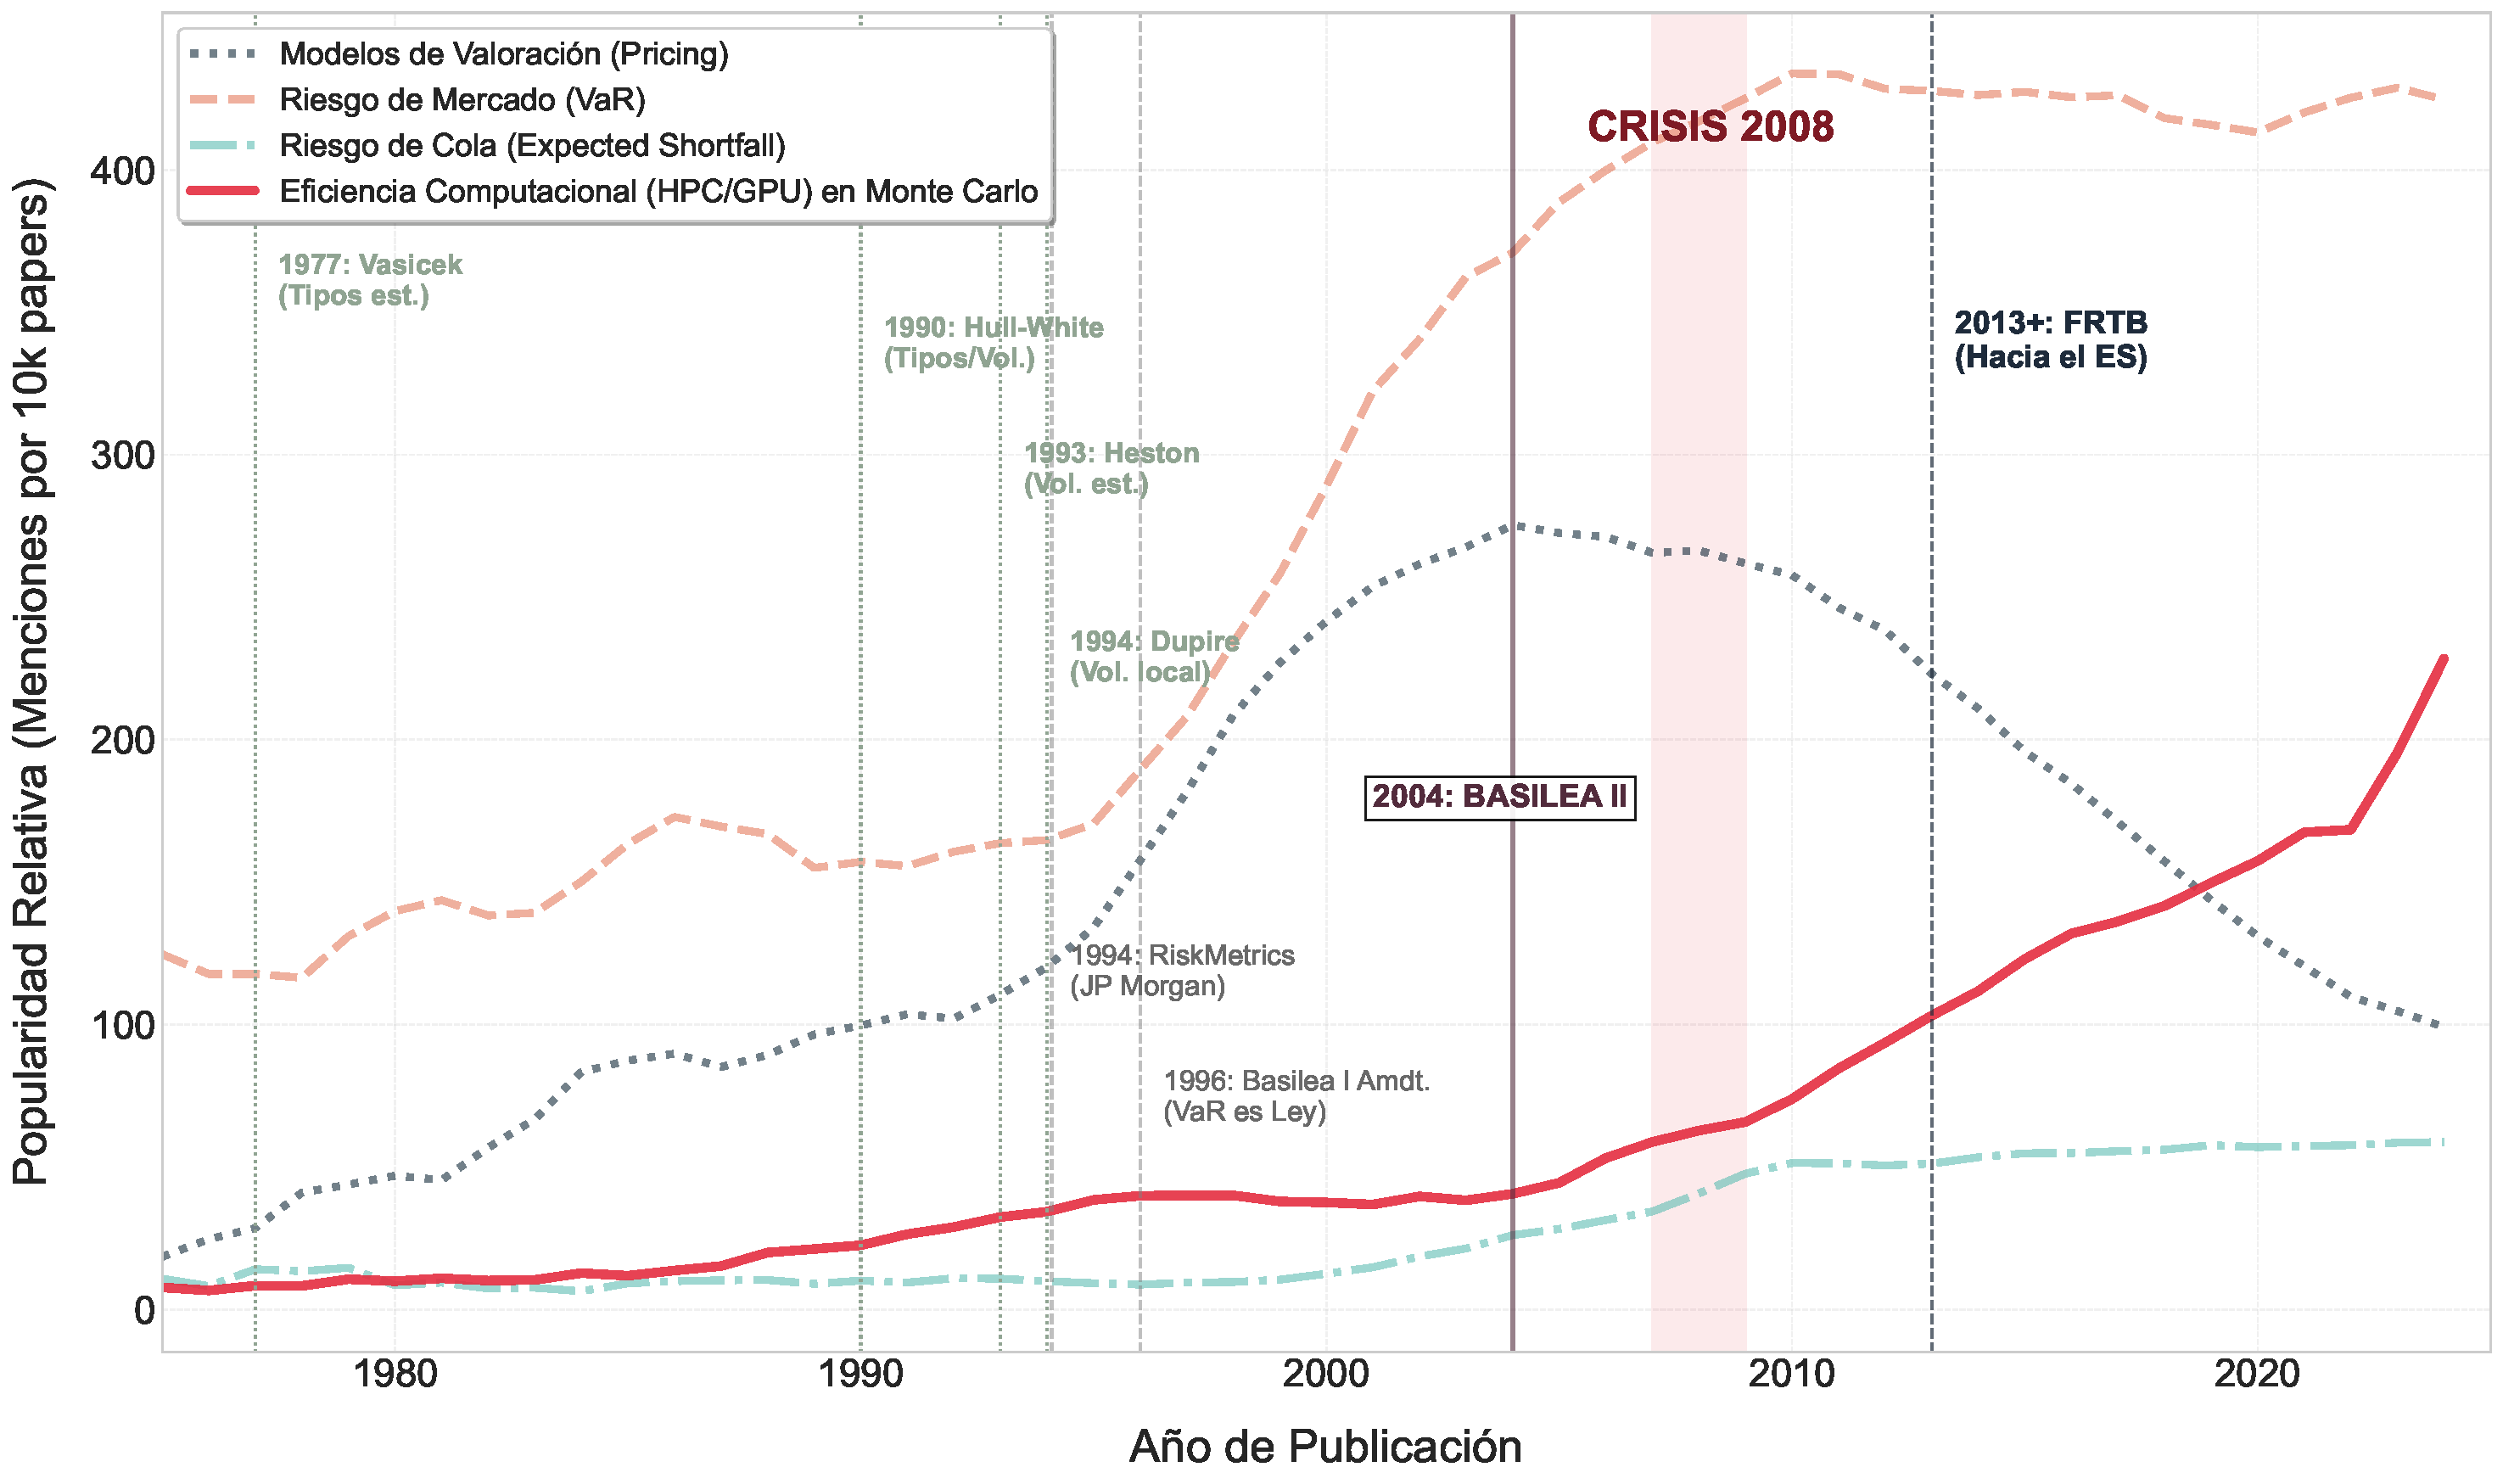
\includegraphics[width=1\textwidth]{Fig5.pdf}
    \caption{Análisis bibliométrico de la evolución temporal de conceptos clave en la literatura financiera cuantitativa (menciones normalizadas por cada 10\,000 artículos).}
    \label{fig:evolucion_cuant_tfm}
\end{figure}

\subsubsection{El pricing analítico y el Monte Carlo clásico (1975--2008)}

Como muestra la curva de trazo discontinuo gris (\textit{Pricing}), las tres décadas posteriores a la publicación del modelo de Black-Scholes-Merton estuvieron dominadas por la búsqueda de soluciones analíticas cerradas. Modelos estructurales como Vasicek (1977) \cite{vasicek1977equilibrium} o Hull-White (1990) \cite{hull1990pricing} para tipos de interés, y Heston (1993) \cite{heston1993closed} o Dupire (1994) \cite{dupire1994pricing} para volatilidad estocástica y local, competían por ofrecer fórmulas directas. 

Sin embargo, a medida que la ingeniería financiera sofisticaba los productos estructurados (opciones de trayectoria dependiente, exóticas y multi-activo), la literatura comenzó a chocar contra la barrera de la intratabilidad matemática. Fue la publicación seminal de Phelim Boyle (1977) \cite{boyle1977options} la que demostró que el método de Monte Carlo era la única alternativa viable para romper esta rigidez en la valoración de derivados complejos. No obstante, como refleja la gráfica, la literatura de \textit{Pricing} alcanzó su cénit absoluto a principios de la década de los 2000 y experimentó un desplome estructural tras la crisis de 2008, marcando el agotamiento definitivo de las soluciones cerradas analíticas.

\subsubsection{La era del riesgo regulatorio y el colapso del supuesto de normalidad (2008--2015)}

De forma inversa al declive del \textit{Pricing}, la curva de puntos naranja (VaR) registra un ascenso vertical que se inicia con la publicación del documento técnico \textit{RiskMetrics} por J.P. Morgan en 1994 \cite{jpmorgan1994riskmetrics} y la enmienda de Basilea de 1996 \cite{bcbs1996amendment}, consolidándose en Basilea II (2004) \cite{bcbs2004basel2}. En esta fase, el método de Monte Carlo mutó su objetivo principal: ya no se utilizaba de forma aislada para valorar una opción individual, sino para generar escenarios macroeconómicos conjuntos que permitieran calcular el VaR de carteras globales. 

La crisis de 2008 supuso un punto de ruptura bibliométrico. Los modelos paramétricos de VaR basados en matrices de varianza-covarianza demostraron ser incapaces de capturar los eventos de cola. La literatura académica reaccionó volcándose en el Expected Shortfall, cuya curva (línea continua azul) experimenta un crecimiento exponencial a partir de las primeras directrices del marco FRTB en 2013 \cite{bcbs2013frtb}. El paso normativo del VaR al 99\% al ES al 97.5\% supuso la consagración del método de Monte Carlo como estándar industrial, al ser el único enfoque metodológico capaz de integrar distribuciones de probabilidad no normales con colas pesadas y dependencias no lineales complejas.

\subsubsection{La era de la eficiencia computacional y la optimización del algoritmo (2015--2026)}

El principal desafío del cálculo del Expected Shortfall mediante simulación de Monte Carlo reside en su elevado coste computacional. Esta exigencia computacional masiva es la causa directa del auge vertical de la curva roja (\textit{Efficiency / HPC}). La literatura científica actual ya no debate sobre la validez matemática del Monte Carlo, sino sobre cómo acelerar su convergencia y su ejecución, lo que constituye la frontera del estado del arte actual en el que se inscribe este trabajo.

\subsection{Fronteras tecnológicas en la aceleración del motor de Monte Carlo}

A medida que el cálculo del Expected Shortfall exigido por el marco FRTB consolidaba al método de Monte Carlo como el estándar indiscutible de la industria, la literatura científica comenzó a buscar alternativas para mitigar su severo coste computacional.

\subsubsection{La hibridación con Machine Learning como respuesta al coste computacional}

En esta búsqueda, la intersección entre el aprendizaje automático y las finanzas cuantitativas no ha surgido como un intento de sustituir por completo la simulación estocástica, sino como una vía para optimizar sus componentes más pesados.

Una de las primeras respuestas maduras en esta dirección fue propuesta por Hejazi y Jackson (2016) \cite{hejazi2016neural}, quienes introdujeron el concepto de metamodelización en el bucle de riesgo. Su enfoque demostró que es posible entrenar redes neuronales artificiales para que aprendan la función de valor de carteras masivas y complejas (como las \textit{variable annuities}). Al hacer esto, el motor de Monte Carlo ya no necesita ejecutar costosos y lentos tasadores numéricos para cada escenario simulado; en su lugar, la red neuronal actúa como un aproximador funcional de velocidad ultra alta. Un salto cualitativo dentro de esta misma corriente lo dieron Huge y Savine (2020) \cite{huge2020differential} con la introducción del \textit{Differential Machine Learning}. Estos autores demostraron que si el modelo de aprendizaje automático se entrena no solo con los precios de salida, sino también con sus derivadas respecto a los factores de riesgo (las sensibilidades financieras o griegas), la red neuronal es capaz de aproximar perfiles de pago fuertemente no lineales con una precisión matemática sin precedentes y utilizando una fracción mínima de escenarios de entrenamiento.

De forma paralela a la aceleración de los tasadores internos, otra corriente de la literatura ha explorado el uso de redes neuronales para predecir directamente las métricas de riesgo sin necesidad de simular toda la distribución. En este ámbito, Chronopoulos, Raftapostolos y Kapetanios (2024) \cite{chronopoulos2024forecasting} propusieron arquitecturas profundas basadas en regresión de cuantiles para pronosticar el VaR, logrando capturar de forma nativa los clústeres de volatilidad y las colas pesadas de los datos de mercado sin imponer restricciones paramétricas previas. Sin embargo, la dependencia de la simulación tradicional sigue siendo un pilar fundamental incluso en los enfoques más disruptivos. Muestra de ello es el reciente trabajo de Barrera, Crépey, Gobet, Nguyen y Saadeddine (2026) \cite{barrera2026statistical}, quienes al formalizar el aprendizaje estadístico conjunto del VaR y el ES, concluyen que para que estas redes profundas aprendan a reaccionar ante escenarios de estrés de forma robusta, es obligatorio entrenarlas utilizando datos sintéticos generados previamente mediante un motor de Monte Carlo clásico.

Esta transición desde los laboratorios académicos hasta las salas de negociación de la banca real queda perfectamente reflejada por García-Muñoz, Gunnesson y Elorza (2026) \cite{garcia2026deep}. En una investigación nacida en el seno del grupo BBVA, los autores analizan los retos prácticos de implementar técnicas de \textit{Deep Learning} para cumplir con las exigencias del marco regulatorio FRTB. Su estudio evidencia que, aunque el Machine Learning permite procesar la re-valoración masiva de carteras globales dentro de los límites de tiempo operativos del banco, la introducción de estos modelos genera un ``riesgo de modelo" crítico debido a la opacidad intrínseca de las estructuras de caja negra. 

Precisamente por este motivo, esta línea de trabajo no se ha considerado en el presente proyecto. Aunque el empleo de técnicas de \textit{Machine Learning} constituye una estrategia prometedora para reducir los tiempos de cálculo, su naturaleza aproximada y la pérdida de interpretabilidad asociada desvían el foco de los objetivos planteados. El propósito de este trabajo es analizar y optimizar el motor de cálculo desde una perspectiva algorítmica y computacional, identificando los factores que limitan su rendimiento y desarrollando técnicas que permitan acelerar su ejecución sin modificar el modelo financiero subyacente ni comprometer la trazabilidad y auditabilidad del proceso.

\subsubsection{Computación cuántica y la búsqueda de la aceleración cuadrática}

En el extremo más vanguardista de la investigación en eficiencia computacional, la literatura científica analiza la computación cuántica como una vía para superar las limitaciones de la simulación estocástica tradicional. El interés de la industria reside en un cambio en las leyes de convergencia: mientras que el método de Monte Carlo clásico presenta un error estadístico de $\mathcal{O}(1/\sqrt{N})$, los algoritmos basados en la estimación de amplitud cuántica (\textit{Quantum Amplitude Estimation}, QAE) prometen una aceleración cuadrática, alcanzando una tasa de convergencia de $\mathcal{O}(1/N)$. En este contexto, Montanaro (2015) \cite{montanaro2015quantum} formalizó los fundamentos matemáticos de esta aceleración, demostrando que puede alcanzarse una misma precisión con un número significativamente menor de escenarios.

La aplicación de este marco al ámbito financiero se ha centrado en diseñar circuitos capaces de cargar distribuciones de probabilidad y valorar instrumentos financieros sobre registros cuánticos. Rebentrost, Gupt y Bromley (2018) \cite{rebentrost2018quantum} propusieron un algoritmo para el \textit{pricing} de derivados, mientras que Woerner y Egger (2019) \cite{woerner2019quantum} extendieron este enfoque al cálculo del VaR y el ES, evaluando su viabilidad mediante simulaciones y pruebas sobre hardware cuántico.

Sin embargo, la aplicación práctica continúa limitada por las restricciones de los procesadores de la era NISQ (\textit{Noisy Intermediate-Scale Quantum}) \cite{preskill2018quantum}, caracterizados por elevados niveles de ruido y decoherencia. Para mitigar estas limitaciones, Suzuki et al. (2020) \cite{suzuki2020amplitude} propusieron una variante de QAE que elimina la etapa de estimación de fase cuántica, reduciendo la profundidad de los circuitos y facilitando su ejecución en el hardware disponible.

La investigación también ha avanzado hacia problemas de mayor dimensión y la agregación de riesgos en carteras diversificadas. Chen, Li y Neufeld (2023) \cite{chen2023quantum} analizaron la complejidad y los errores del Monte Carlo cuántico aplicado a las ecuaciones de Black-Scholes para opciones multi-activo, mientras que Zhu et al. (2023) \cite{zhu2023copula} incorporaron modelos de agregación mediante cópulas en ordenadores cuánticos de iones atrapados para representar dependencias no lineales y colas pesadas.

No obstante, revisiones recientes, como la de Gong, Sedai, Schroeder y Medda (2026) \cite{gong2026quantum}, concluyen que la ventaja cuántica frente a los sistemas clásicos sigue dependiendo de la disponibilidad de hardware tolerante a fallos y de gran escala.

Por este motivo, la computación cuántica tampoco se ha considerado como una línea de desarrollo dentro del presente proyecto. Aunque se han realizado algunas pruebas exploratorias, el estado actual de esta tecnología la sitúa fuera del ámbito de aplicación práctica de este trabajo.

\subsubsection{Optimización algorítmica y computación de alto rendimiento en el Monte Carlo clásico}

Frente a las líneas de investigación basadas en la opacidad del \textit{Machine Learning} o la inmadurez de la computación cuántica, la corriente principal de la industria financiera se ha concentrado en optimizar el método de Monte Carlo desde su propia raíz algorítmica y arquitectónica. Esta vertiente, responsable del auge vertical de la curva de eficiencia e infraestructura reflejada en el análisis bibliométrico, demuestra que el margen de mejora en sistemas de cómputo tradicionales sigue siendo crítico para el cumplimiento de normativas como FRTB.

En el plano matemático, una de las palancas más extendidas para mejorar la eficiencia estadística del Monte Carlo---sin sustituir el tasador---consiste en reducir la varianza del estimador o, equivalentemente, alcanzar mayor precisión con el mismo número de escenarios.
En este contexto, las secuencias de baja discrepancia de Sobol \cite{sobol1967on} combinadas con puentes brownianos son una de las principales vías del conocido cuasi-Monte Carlo \cite{boyle1997monte, glasserman2003monte}. Las variables antitéticas \cite{hammersley1956new}, por su parte, constituyen un mecanismo sencillo y de coste marginal que aprovecha la simetría de las leyes normales para estabilizar la estimación. 

Conjuntamente, estas técnicas constituyen el referente estándar en ingeniería financiera cuando el objetivo es aproximar cuantiles y medias de cola---como el VaR o el ES---con un presupuesto computacional acotado; el presente trabajo las adopta como núcleo metodológico y las desarrolla en los capítulos de diseño y resultados.

Otra familia de métodos, complementaria pero de naturaleza distinta, es el enfoque multinivel (\textit{Multilevel Monte Carlo}, MLMC). Giles (2015) \cite{giles2015multilevel} sistematizó las bases de esta técnica, demostrando que es posible distribuir la simulación a lo largo de una jerarquía de niveles con diferentes grados de resolución o discretización temporal. Al realizar la mayor parte de los muestreos en niveles burdos de bajo coste y reservar un número reducido de trayectorias para los niveles más finos y precisos, el método MLMC logra reducir drásticamente la varianza del estimador global sin perder precisión. La versatilidad de este enfoque ha propiciado desarrollos avanzados en la literatura, donde Jasra, Law y Suciu (2020) \cite{jasra2020advanced} extendieron el marco multinivel hacia problemas estadísticas complejos y modelos de filtrado no lineales, ampliando su estabilidad matemática. De igual modo, Jeng y Kiliçman (2021) \cite{jeng2021multilevel} combinaron las bondades del método MLMC con técnicas tradicionales de variables de control (\textit{control variates}) para la valoración de opciones bajo entornos de volatilidad rugosa (\textit{rough Heston model}), evidenciando que la hibridación algorítmica interna permite optimizar la convergencia incluso bajo dinámicas de mercado altamente complejas.

En paralelo a la eficiencia matemática, el rediseño del algoritmo para su adaptación a arquitecturas de hardware de última generación constituye el otro gran motor de eficiencia de la industria. Un reflejo disruptivo de esta tendencia es el trabajo de Belletti et al. (2020) \cite{belletti2020tensor}, quienes evaluaron el uso de Unidades de Procesamiento de Tensores (TPU) —diseñadas originalmente para el aprendizaje profundo— aplicadas a la simulación de Monte Carlo en finanzas. Estos autores demostraron que, si el generador de números aleatorios y las funciones de pago se reformulan vectorialmente como operaciones de álgebra lineal masiva, es posible explotar la arquitectura de los aceleradores de Google para procesar carteras globales a velocidades órdenes de magnitud superiores a las de las CPUs convencionales.

Finalmente, la literatura más reciente confirma que la optimización del software en producción no solo busca acelerar la métrica de riesgo base (VaR o ES), sino también las métricas de sensibilidad asociadas, vitales para las mesas de negociación. En este ámbito, Vandendorpe (2026) \cite{vandendorpe2026efficient} propuso un algoritmo altamente eficiente para el cálculo de las griegas de correlación (\textit{correlation Greeks}) dentro de entornos computacionales financieros. Su enfoque reduce el coste computacional de evaluar cómo reacciona la cartera ante cambios en la matriz de interdependencias de los activos, un problema que tradicionalmente multiplicaba el número de simulaciones de Monte Carlo necesarias y que ahora puede resolverse de manera optimizada.

Este marco de optimización algorítmica y aprovechamiento del hardware tradicional es el escenario exacto en el que se inscribe este Trabajo de Fin de Máster. Al centrar el desarrollo en C++, el proyecto adopta los principios de la literatura que abogan por el control total de la infraestructura: diseñar generadores de números pseudoaleatorios eficientes que eviten el estado compartido y estructurar el motor mediante paralelismo nativo en CPU. De esta forma, se demuestra que la optimización del software clásico sigue siendo la vía más robusta, transparente y auditable para dar respuesta a los desafíos computacionales de la gestión de riesgos contemporánea.

\section{Metodología y Stack Tecnológico}
    \subsection{Marco metodológico de trabajo}

Para el desarrollo del motor de simulación de Monte Carlo, opté por un ciclo de vida del software de carácter iterativo e incremental, adaptado específicamente a las necesidades de la ingeniería cuantitativa. Este enfoque me permitió mitigar el riesgo de arrastrar errores lógicos o de cálculo desde las fases tempranas, asegurando la robustez matemática del motor antes de comprometer esfuerzos en la optimización de bajo nivel. 

Aunque la implementación comenzó desde etapas tempranas, previamente se definieron los objetivos funcionales del sistema, los principales módulos que lo compondrían y las responsabilidades de cada uno de ellos. Esta planificación inicial sirvió como guía para mantener una arquitectura modular y escalable durante todo el desarrollo.

El flujo de trabajo seguido se estructuró en tres fases principales:

\begin{enumerate}
\item \textbf{Prototipado y validación matemática:}

La primera fase consistió en desarrollar un prototipo simplificado en Python. El objetivo principal no era alcanzar un elevado rendimiento computacional, sino validar la corrección matemática de los algoritmos de simulación y de los procedimientos estadísticos empleados. A partir de este prototipo se generó un conjunto de resultados de referencia que posteriormente se utilizó para contrastar la precisión de las implementaciones definitivas.

\item \textbf{Implementación modular en C++ y validación continua:}

Una vez verificadas las bases matemáticas, se desarrolló la implementación principal en C++. La construcción del sistema se realizó de forma modular, separando claramente los generadores de trayectorias, los modelos estocásticos, los mecanismos de valoración y los componentes estadísticos. Cada módulo fue incorporándose progresivamente al sistema y validándose frente a los resultados de referencia obtenidos durante la fase anterior. Para garantizar la estabilidad del código durante las sucesivas iteraciones, se integró un conjunto de pruebas unitarias (\textit{unit tests}) que permitió detectar regresiones y verificar el correcto funcionamiento de cada componente.

\item \textbf{Optimización y análisis de rendimiento:}

Con una versión funcional y validada del motor, la última fase se centró en la mejora de la eficiencia computacional. Se revisaron aspectos relacionados con la gestión de memoria, la minimización de copias innecesarias mediante semántica de movimiento, la organización de estructuras de datos para favorecer la localidad de referencia y la paralelización de las simulaciones. El objetivo de esta etapa fue maximizar el rendimiento del cálculo de métricas de riesgo como el VaR y el Expected Shortfall sin comprometer la mantenibilidad del código.

\end{enumerate}

\subsubsection*{Uso de herramientas de IA generativa durante el desarrollo}
Puesto que, en el flujo de trabajo se ha hecho uso de IA generativa, se incluye el anexo plantilla de uso responsable al final del documento. 

\subsection{Especificación de requisitos}

Aunque en la introducción ya hemos comentado brevemente los objetivos de este trabajo, en este apartado comentamos en mayor profundidad los requisitos con el fin de poder garantizar la viabilidad técnica del motor de simulación y su correcto alineamiento con las necesidades del análisis de riesgos financiero, separando en una serie de requisitos funcionales (el qué hace el sistema) y no funcionales (el cómo lo ejecuta a nivel de rendimiento y arquitectura).

\subsubsection{Requisitos funcionales}

Los requisitos funcionales determinan el comportamiento operativo del motor, la flexibilidad de los modelos matemáticos que soporta y la capacidad de parametrización de las métricas cuantitativas:

\begin{itemize}
    \item \textbf{Modelización y simulación de activos:}
    \begin{itemize}
        \item \textbf{Activos individuales:} El sistema debe simular la evolución del precio de activos financieros independientes siguiendo la dinámica del Movimiento Browniano Geométrico (GBM). Estos activos deben poder ser el subyacente de derivados financieros tales como opciones europeas u opciones barrera. Además, se deben poder incluir en la cartera elementos de renta fija como bonos \cite{options2018hull}.
        \item \textbf{Carteras multifactoriales:} El motor debe permitir la simulación conjunta de carteras de activos correlacionados. Esta interdependencia lineal se gestiona mediante la lectura y procesamiento de una matriz de correlación integrada en la configuración del simulador (\texttt{MontecarloEngine.h} y \texttt{MontecarloEngine.cpp}).
        \item \textbf{Dinámica de tipos de interés:} El software debe dar soporte a la modelización estocástica de curvas de tipos de interés mediante la activación opcional del modelo de Hull-White \cite{options2018hull}. Esto se parametriza a través del campo \texttt{rateModel} dentro de la estructura de configuración global \texttt{SimConfig}, procesándose en los módulos \texttt{HullWhiteModel.cpp} y \texttt{MontecarloEngine.h}.
    \end{itemize}

    \item \textbf{Cálculo continuo de métricas de riesgo (VaR y ES):}
    El módulo de análisis estadístico (\texttt{RiskCalculator.cpp}) no debe verse limitado por un conjunto estático de niveles de confianza. El requisito funcional exige que tanto el VaR como el Expected Shortfall puedan ser calculados de forma dinámica para cualquier percentil continuo dentro del rango abierto $(0, 1)$. Para los entornos de pruebas y regresión del proyecto, se establecen como estándares de validación regulatoria los niveles del $99\%$ para el VaR y $97.5\%$ para el ES \cite{bcbs2013frtb}.

    \item \textbf{Flexibilidad del horizonte temporal:}
    El motor debe permitir la simulación de múltiples escenarios temporales sin necesidad de recompilar el código. Ajustando las variables \texttt{totalTime} (horizonte temporal total) y \texttt{numSteps} (número de pasos de discretización) expuestas en la estructura \texttt{SimConfig}, el usuario debe ser capaz de configurar simulaciones equivalentes a plazos de 1 día, 10 días o 1 año de forma dinámica, tal y como se verifica en las ejecuciones de \texttt{test\_acciones.cpp}.
\end{itemize}

\subsubsection{Requisitos técnicos}

Los requisitos no funcionales delimitan las restricciones operativas, la eficiencia computacional, la gestión de recursos físicos de la máquina y la viabilidad de la infraestructura de compilación:

\begin{itemize}
    \item \textbf{Rendimiento computacional y análisis experimental:}
    El motor debe demostrar escalabilidad computacional y convergencia estadística medibles sobre el escenario \texttt{benchmark1} y el entorno de hardware de referencia (Tabla~\ref{tab:hardware}). En lugar de fijar \emph{service level agreements} (SLA) absolutos de latencia en producción ---ajenos al alcance académico del TFM---, se establecen criterios de aceptación numéricos ex ante en la Tabla~\ref{tab:criterios_aceptacion}, vinculados a la \textit{suite} de pruebas (\texttt{integration\_tests}, \texttt{standard\_error\_tests}) y contrastados empíricamente en el Capítulo~6. Los benchmarks evalúan el comportamiento del generador de números aleatorios (RNG), la eficiencia del paralelismo bajo la ley de Amdahl \cite{amdahl1967validity} y el impacto del layout de memoria.
    
    \item \textbf{Gestión de la compilación y portabilidad (CMake):}
    El proyecto requiere el uso de \texttt{CMake} \cite{cmake_software} para automatizar y estructurar la construcción del ejecutable y la \textit{suite} de pruebas unitarias. No obstante, no se utilizará un gestor automático de dependencias, por lo que de cara a la portabilidad sería necesario modificar alguna ruta en el \texttt{CMakeLists.txt} para localizar las librerías externas (modificar la ruta de dichas librerías) como \texttt{Boost} \cite{boost_libraries} y \texttt{Eigen} \cite{eigenweb}. El software cumple el requisito de sentar las bases analíticas para un despliegue multiplataforma e Integración Continua (CI), pero requiere una refactorización futura para eliminar dicho acoplamiento local.

    \item \textbf{Eficiencia en el consumo de memoria RAM y localidad de caché:}
    La simulación de Monte Carlo puede saturar rápidamente los recursos de hardware si no se gestiona correctamente. Para mitigar esto, se imponen las siguientes restricciones de diseño:
    \begin{itemize}
        \item \textbf{Persistencia optimizada:} El motor, cuando sea posible, solo debe almacenar en memoria el P\&L (\textit{Profit and Loss}) final acumulado por trayectoria para el cálculo de los percentiles, evitando la retención global de las matrices que contienen los paths completos.
        \item \textbf{Localidad de datos:} Se exige el uso de un almacenamiento en disposición por filas (\texttt{RowMajor}) para maximizar el acierto de la caché (\textit{cache hits}) del procesador, junto con la pre-reserva explícita de memoria en vectores y \textit{buffers} reutilizables dentro de cada batch de ejecución.
        \item \textbf{Coste transitorio aceptado:} Se asume como restricción que, durante la valoración de carteras, se construirán vectores temporales para las trayectorias de cada activo. Esto implica que la memoria transitoria escalará de forma proporcional al tamaño de la cartera y al número de pasos temporales configurados. %AQUÍ CUIDADO TAMBIÉN
    \end{itemize}
\end{itemize}

\subsubsection{Criterios de aceptación verificables}

Los requisitos técnicos anteriores se operacionalizan mediante los identificadores \texttt{CA-XX} de la Tabla~\ref{tab:criterios_aceptacion}. Cada fila fija un umbral numérico comprobable \emph{antes} de la campaña experimental del Capítulo~6, el artefacto de verificación (test automatizado o benchmark reproducible) y la sección donde se reporta el cumplimiento. Los criterios no pretenden certificar despliegue industrial, sino demostrar de forma auditable que el motor satisface los objetivos de precisión estadística y eficiencia computacional declarados en la §1.2.

\begin{table}[h]
\centering
\small
\setlength{\tabcolsep}{4pt}
\begin{tabularx}{\textwidth}{|l|X|c|l|}
\hline
\textbf{ID} & \textbf{Criterio de aceptación (umbral)} & \textbf{Escenario} & \textbf{Evidencia (Cap.~6)} \\ \hline
CA-01 &
Con $N=2\,048$, la banda $\pm\,\text{SE}$ del $\text{VaR}_{99\%}$ con Sobol es al menos un $30\,\%$ más estrecha que con Mersenne Twister. &
\texttt{benchmark1}, HW &
§6.2, Fig.~\ref{fig:convergencia_var_es} \\ \hline
CA-02 &
Con $N=2^{17}$, el error relativo $\text{SE}/|\hat{\text{ES}}|$ del $\text{ES}_{97{,}5\%}$ bajo Sobol es $< 0{,}05\,\%$. &
\texttt{benchmark1}, HW &
§6.2, Fig.~\ref{fig:convergencia_var_es} \\ \hline
CA-03 &
El ajuste log--log del error relativo del $\text{ES}_{97{,}5\%}$ con Sobol verifica un exponente $\alpha < -0{,}55$ (por debajo de $\mathcal{O}(N^{-1/2})$). &
\texttt{benchmark1}, HW &
§6.2, Fig.~\ref{fig:convergencia_var_es} \\ \hline
CA-04 &
Speedup empírico $S(8)=T_1/T_8 \ge 4{,}0$ con $N=10^5$ simulaciones. &
\texttt{benchmark1} &
§6.3, Fig.~\ref{fig:paralelismo_speedup} \\ \hline
CA-05 &
Fracción paralelizable del ajuste de Amdahl $P \ge 0{,}85$. &
\texttt{benchmark1} &
§6.3, Fig.~\ref{fig:paralelismo_speedup} \\ \hline
CA-06 &
Ratio de tiempos ColMajor/RowMajor $\ge 1{,}20$ con $2\,048$ activos ($512$ réplicas de \texttt{benchmark1}). &
Cartera replicada &
§6.3, Fig.~\ref{fig:benchmark_layout_speedup_activos} \\ \hline
CA-07 &
Las tres configuraciones RNG (MT, antitéticas, Sobol) convergen hacia el mismo orden de magnitud de $\text{VaR}_{99\%}$ y $\text{ES}_{97{,}5\%}$ (sin sesgo sistemático apreciable entre generadores). &
\texttt{benchmark1}, HW &
§6.2, Fig.~\ref{fig:convergencia_var_es} \\ \hline
\end{tabularx}
\caption{Criterios de aceptación numéricos del motor: umbrales ex ante y evidencia empírica en el Capítulo~6.}
\label{tab:criterios_aceptacion}
\end{table}
\subsection{Instrumentos, técnicas y herramientas empleadas}

Para la materialización del motor de simulación, se seleccionó un \textit{stack} tecnológico fundamentado en el ecosistema nativo de C++, priorizando la eficiencia en el cálculo numérico y el control absoluto sobre la gestión de memoria y la concurrencia. A continuación, se detallan las herramientas, librerías y el entorno de ingeniería de software que componen la infraestructura del proyecto.

\subsubsection{Estándar del lenguaje y características nativas}

El núcleo del motor de Monte Carlo se ha desarrollado bajo el estándar \textbf{GNU C++20}, configurado explícitamente en el archivo de automatización mediante la directiva \texttt{-std=gnu++20} en el script \texttt{CMakeLists.txt}. Esta elección proporciona un entorno de compilación maduro y altamente compatible, permitiendo explotar características esenciales del lenguaje:

\begin{itemize}
    \item \textbf{Concurrencia y multihilo nativo:} Para combatir la alta demanda computacional de las simulaciones, se implementa en \texttt{MontecarloEngine.cpp} un modelo de paralelismo asíncrono nativo utilizando las abstracciones de alto nivel de la librería estándar: \texttt{std::thread}, \texttt{std::future} y \texttt{std::async}. Esto permite distribuir los lotes (\textit{batches}) de trayectorias entre los diferentes hilos de procesamiento de la CPU de forma eficiente, reduciendo drásticamente el tiempo de ejecución sin incurrir en la sobrecarga de librerías externas de paralelismo.
    \item \textbf{Generación de pseudoaleatoriedad estándar:} En el componente \texttt{RandomGenerator.h} se explotan las utilidades nativas de la cabecera \texttt{<random>}, empleando el motor de Mersenne Twister de 64 bits (\texttt{std::mt19937\_64}) junto con la distribución normal estándar \\(\texttt{std::normal\_distribution}) para asegurar una base estocástica de alta calidad y rendimiento en las simulaciones probabilísticas tradicionales.
\end{itemize}

\subsubsection{Librerías externas especializadas}

Con el fin de no reinventar componentes numéricos complejos y garantizar la máxima optimización algebraica, el proyecto se apoya en dos librerías fundamentales dentro del entorno cuantitativo:

\begin{itemize}
    \item \textbf{Eigen (Álgebra Lineal) \cite{eigenweb}:} Integrada en \texttt{MontecarloEngine.cpp}, esta librería de plantillas de C++ se emplea para la manipulación y almacenamiento de las matrices de correlación financiera. Su uso es crítico para ejecutar la descomposición de Cholesky mediante el algoritmo $LL^T$ \cite{higham2009cholesky} . Esta operación matemática es la que me permite transformar variables aleatorias independientes en factores de riesgo correlacionados, modelizando con rigor carteras multifactoriales.
    \item \textbf{Boost C++ Libraries \cite{boost_libraries}:} Se utiliza de forma estratégica en dos vertientes del proyecto:
    \begin{itemize}
        \item \textit{Simulación Cuasi-Monte Carlo:} En \texttt{RandomGenerator.h} se importa el módulo \\ \texttt{boost::random::sobol} para la generación de secuencias de baja discrepancia de Sobol. Esto dota al motor de una alternativa avanzada de muestreo que acelera significativamente la convergencia matemática frente al muestreo pseudoaleatorio tradicional.
        \item \textit{Suite de Testing:} En el entorno de desarrollo se emplea el \textbf{Boost Unit Test Framework} para estructurar y automatizar la ejecución de los tests unitarios y de integración desde el \texttt{CMakeLists.txt}.
    \end{itemize}
\end{itemize}

%\subsubsection{Flujo e interfaz de entrada y salida de datos}

%Una decisión clave en el diseño de la arquitectura fue el desacoplamiento total del núcleo del motor de cualquier sistema de archivos o formatos de serialización (como JSON o bases de datos). 

%El núcleo del simulador (\texttt{MontecarloEngine.h}) está diseñado para operar estrictamente en memoria, recibiendo sus parámetros de entrada exclusivamente mediante la estructura \texttt{SimConfig} y los correspondientes objetos de tipo cartera y activos financieros. Este enfoque garantiza que el \textit{core} sea ultrarrápido y agnóstico respecto a la procedencia de los datos.

%Por otro lado, la persistencia y la interfaz con el exterior se gestionan en la capa de pruebas e instrumentación (\texttt{test\_acciones.cpp}). Aquí, haciendo uso de los flujos estándar de C++ (\texttt{<iostream>} y \texttt{<fstream>}), se capturan las métricas de los \textit{benchmarks} de rendimiento y se exportan de forma nativa a archivos en formato CSV. Finalmente, este flujo se conecta con un entorno de análisis cuantitativo en \textit{Python}, donde mediante la librería \textit{Pandas} y entornos de \textit{Jupyter Notebooks} se realiza la lectura, tratamiento estadístico final y representación gráfica de las curvas de convergencia y distribución de pérdidas.

\subsubsection{Entorno de desarrollo y cadena de herramientas (\textit{Toolchain})}

Para la construcción, compilación y depuración del sistema en un entorno local, se configuró la siguiente infraestructura de ingeniería de software:
\begin{itemize}
    \item \textbf{Compilador:} GCC (\textit{GNU Compiler Collection}) en su distribución para Windows a través de \textbf{MinGW-w64} (\texttt{c++.exe}).
    \item \textbf{Sistema de Construcción:} El proceso es coordinado por \textbf{CMake} como generador de abstracción de alto nivel, el cual delega la compilación nativa en la herramienta \textbf{mingw32-make}.
    \item \textbf{Entorno de Desarrollo (IDE):} Todo el flujo de trabajo, la escritura del código y la inspección de variables del sistema se ha centralizado bajo el entorno \textbf{Visual Studio Code}, explotando sus extensiones nativas para C++ y CMake.
\end{itemize}
% --- BLOQUE 2: NÚCLEO TÉCNICO (El "Corazón" del TFM) ---

\section{Diseño y Desarrollo de la Solución}

\subsection{Arquitectura del sistema propuesto y flujo de ejecución}

Para evitar el acoplamiento rígido de componentes —un defecto común en los motores de simulación académicos—, el sistema se ha diseñado bajo un enfoque modular y orientado a objetos, distribuyendo las responsabilidades en componentes independientes y especializados. El flujo de vida del dato dentro del motor se puede estructurar en tres fases secuenciales: configuración y carga, orquestación y simulación, y análisis de riesgo en colas.

A continuación, se detallan las responsabilidades de los módulos principales que gobiernan el sistema:

\begin{itemize}
  \item \textbf{Cápsula de configuración (\texttt{SimConfig}).}
  Estructura de datos ligera que centraliza los parámetros de la simulación y elimina variables codificadas en el código (\emph{hardcoded}).
  Almacena el horizonte temporal (\texttt{totalTime}), el número de pasos (\texttt{numSteps}), el tamaño muestral (\texttt{totalSims}), la matriz de correlación (\texttt{corrMatrix}), el paralelismo (\texttt{numCores}), el generador aleatorio (\texttt{rngType}, \texttt{rngSeed}), el \emph{layout} de la matriz de shocks (\texttt{matrixLayout}) y, de forma opcional, un modelo de tipos de interés (\texttt{rateModel}) y la estimación de errores estándar de VaR/ES (\texttt{computeStandardErrors}, \texttt{bootstrapReplications}, \texttt{sobolBatchCount}).

  \item \textbf{Modelización de activos (\texttt{Asset} y derivadas).}
  La clase base abstracta \texttt{Asset} define la interfaz polimórfica de cualquier factor de riesgo.
  Las implementaciones concretas incluyen \texttt{GBMAsset} (movimiento browniano geométrico), \texttt{EuropeanOption}, \texttt{BarrierOption} (up-and-out call) y \texttt{CouponBond} (modo YTM o precio vía modelo de tipos).
  El método \texttt{simulateFinalValue} constituye el \emph{hot path} invocado por la cartera;  \texttt{generatePath} se reserva para tests y análisis (\emph{cold path}).
  Esta jerarquía permite que el motor sea agnóstico respecto al modelo estocástico de cada instrumento.

  \item \textbf{Agregación en cartera (\texttt{Portfolio}, \texttt{Position}).}
  \texttt{Portfolio} agrupa posiciones (\texttt{Position}), cada una con un \texttt{shared\_ptr<Asset>} y una cantidad.
  El método \texttt{simulatePathPnL} calcula el P\&L de una trayectoria: valora cada activo mediante \texttt{simulateFinalValue}, aplica descuento opcional con \texttt{InterestRateModel} y resta el valor inicial de la cartera.

  \item \textbf{Tipos de interés (\texttt{InterestRateModel}, \texttt{HullWhiteModel}).}
  Interfaz abstracta para simular la trayectoria del tipo corto, descontar flujos y valorar bonos.
  La implementación \texttt{HullWhiteModel} compone una \texttt{YieldCurve} de mercado.
  Su uso es opcional: cuando \texttt{SimConfig.rateModel} está activo, la matriz de correlación incorpora un factor adicional para el driver browniano del tipo.

  \item \textbf{Aleatoriedad (\texttt{RandomGenerator} y utilidades).}
  \texttt{MersenneTwisterGen} y \texttt{BoostSobolGenerator} implementan la interfaz \texttt{RandomGenerator}.
  El motor selecciona el generador según \texttt{rngType}: Mersenne Twister, variables antitéticas (pares $(Z,-Z)$) o secuencias de Sobol.
  En el modo Sobol, \texttt{BoostSobolGenerator} transforma uniformes cuasi-aleatorios mediante \texttt{MathUtils::inverseNormalCDF} y \texttt{MonteCarloEngine} aplica \texttt{BrownianBridge} por factor antes de la correlación.

  \item \textbf{Núcleo de orquestación (\texttt{MonteCarloEngine}).}
  Punto de entrada \texttt{run(const Portfolio\&, const SimConfig\&)}.
  Recibe una cartera ya construida (no la instancia), descompone la correlación con Cholesky ($Z_{\mathrm{corr}} = L Z_{\mathrm{indep}}$), paraleliza batches con \texttt{std::async} y coordina RNG, trayectorias de tipos y llamadas a \texttt{Portfolio::simulatePathPnL}.
  Es aquí donde se integran las técnicas de reducción de varianza y el bucle crítico de Monte Carlo.

  \item \textbf{Consumidor de riesgo (\texttt{RiskCalculator}, \texttt{MonteCarloErrorPolicy}).}
  Módulo de análisis posterior a la simulación.
  Recibe el vector de P\&L simulados (no una matriz), los ordena y calcula VaR$_\alpha$ y ES$_\alpha$ empíricos para $\alpha \in (0,1)$.
  Cuando \texttt{computeStandardErrors} está activo, \texttt{MonteCarloErrorPolicy} estima errores estándar según el esquema asociado al \texttt{rngType} (muestras independientes, pares antitéticos o medias por lotes Sobol), devolviendo \texttt{RiskEstimate} con valor y error.
  Las operaciones estadísticas quedan así aisladas de la lógica de simulación.
\end{itemize}

Como se aprecia en las Figuras~\ref{fig:uml_dominio} y~\ref{fig:uml_engine}, la interacción entre componentes modela el flujo de dependencias del software: el dominio financiero (activos, cartera y tipos) se desacopla del motor, que a su vez delega las métricas en \texttt{Metrics}.
El orquestador central gobierna el ciclo de vida de la simulación sin violar el principio de responsabilidad única.

\begin{figure}[H]
    \centering
    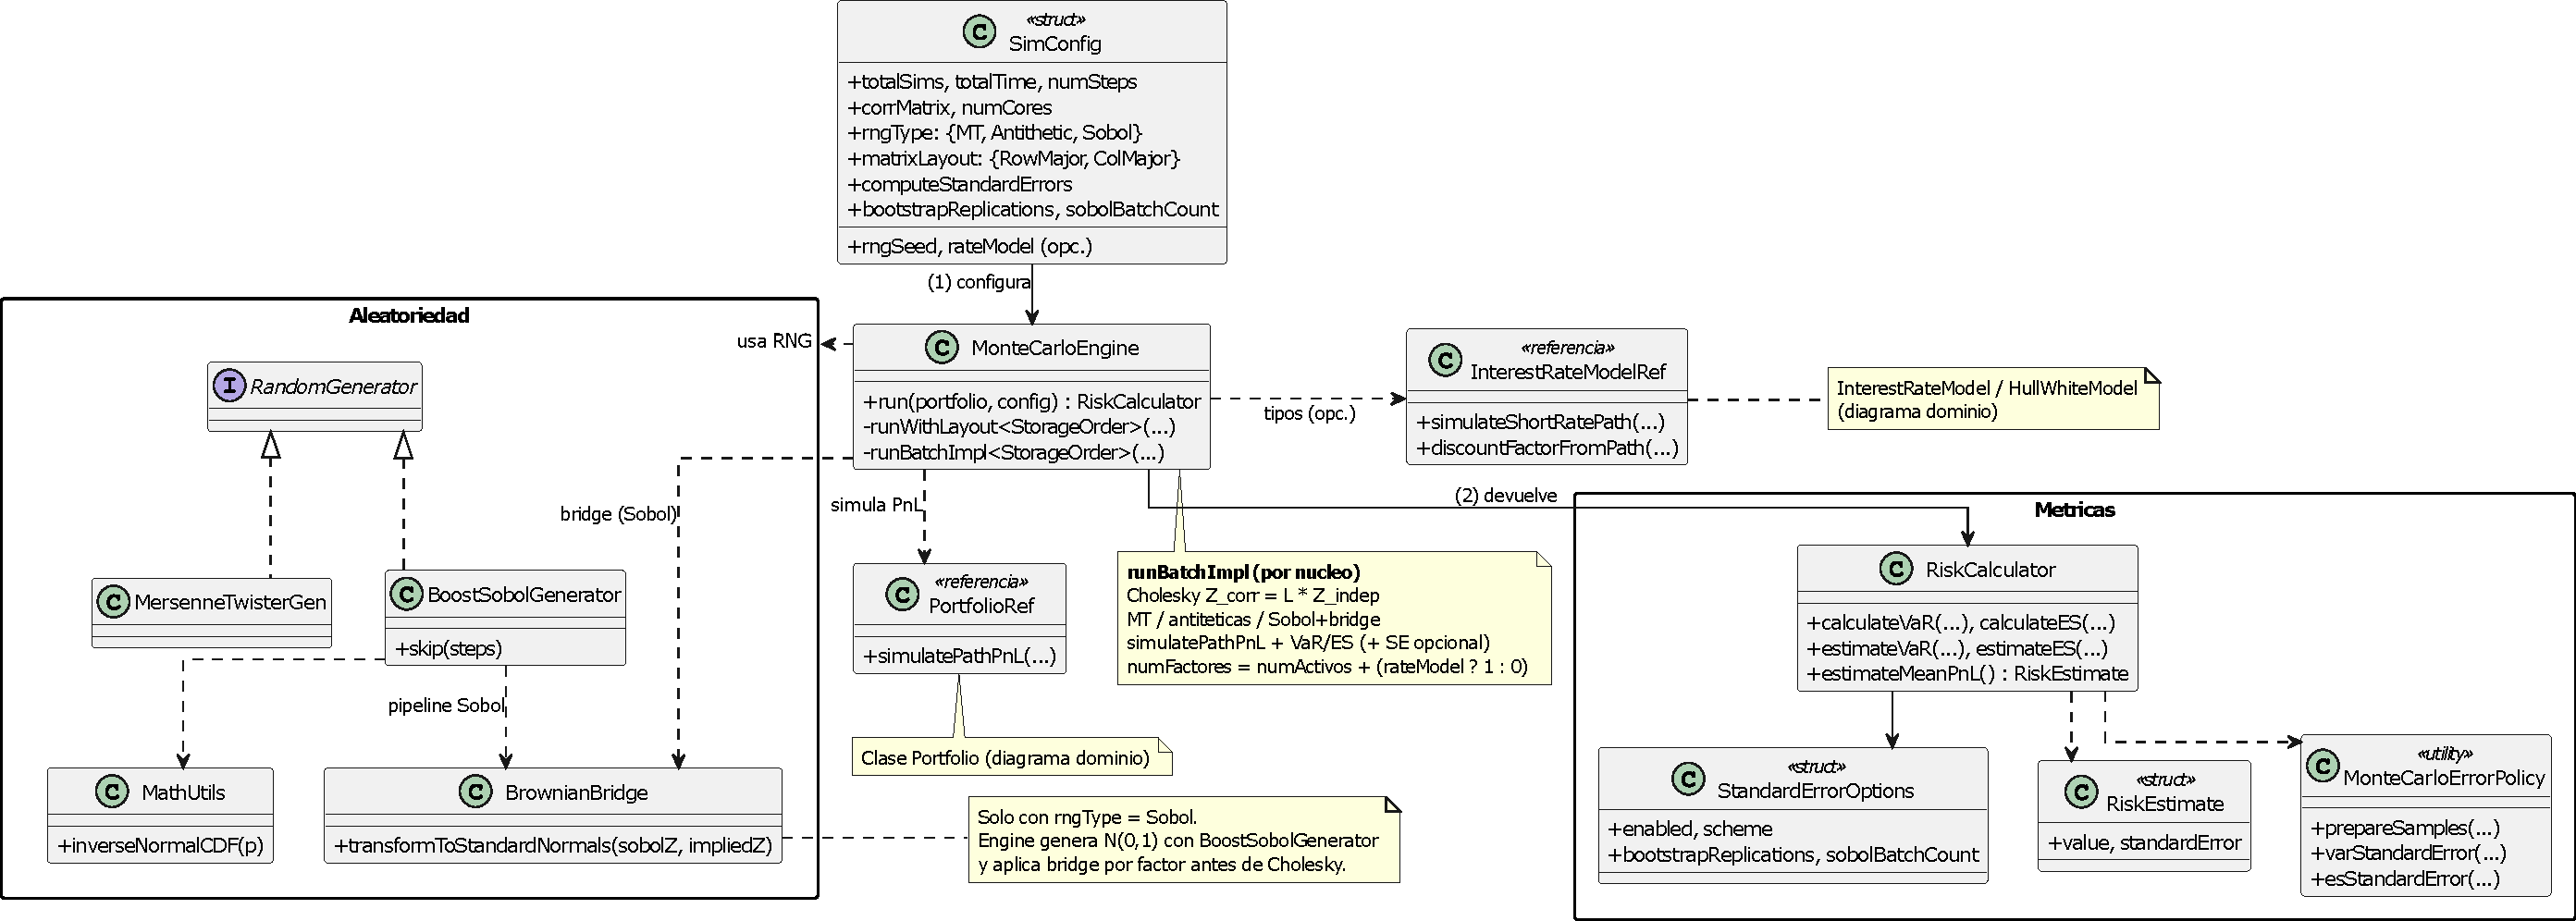
\includegraphics[width=1\linewidth]{Fig6.pdf}
    \caption{Diagrama UML de clases del \emph{motor de simulación}: configuración (\texttt{SimConfig}), orquestación (\texttt{MonteCarloEngine}), generación aleatoria (MT, antitéticas, Sobol y \texttt{BrownianBridge}) y cálculo de métricas de riesgo (\texttt{RiskCalculator}, \texttt{MonteCarloErrorPolicy}).}    
    \label{fig:uml_engine}
\end{figure}

\begin{figure}[H]
    \centering
    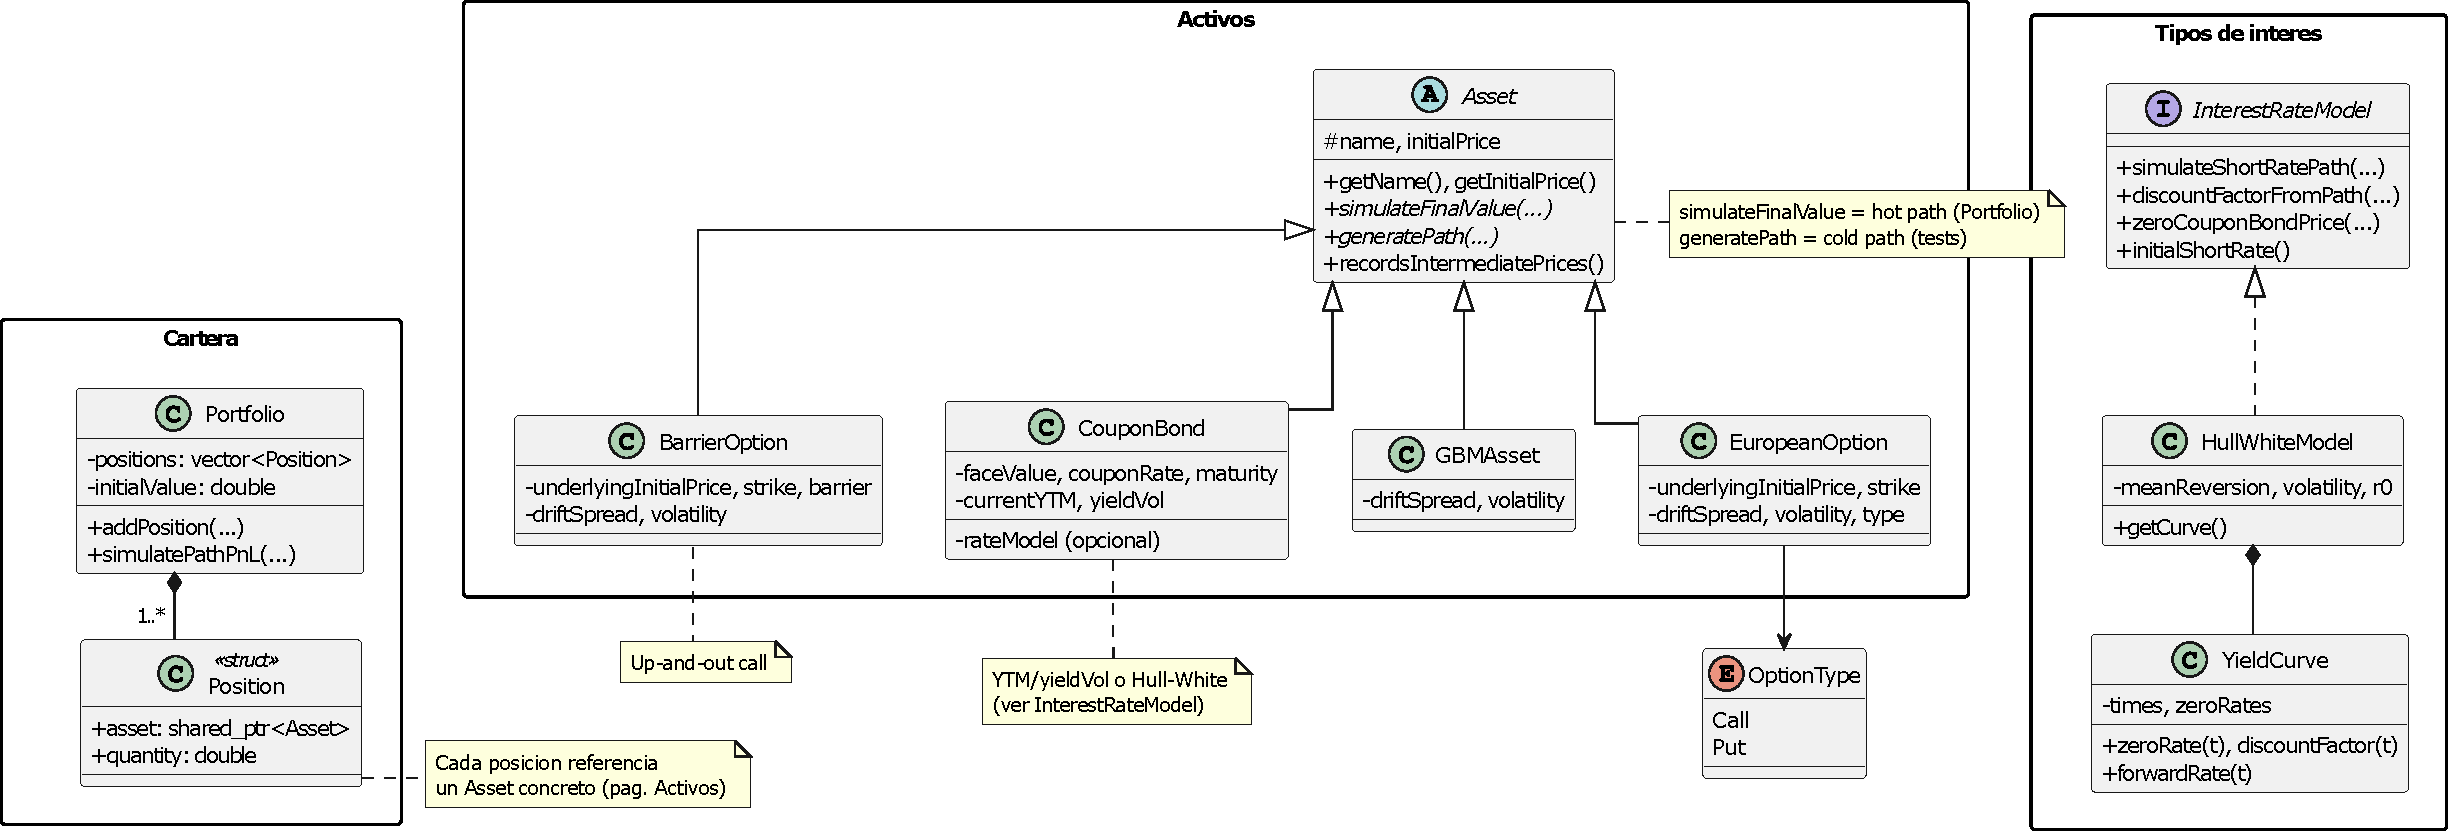
\includegraphics[width=1\linewidth]{Fig7.pdf}
    \caption{Diagrama UML de clases del \emph{modelo de dominio}: jerarquía de activos (\texttt{Asset} y derivadas), agregación en cartera (\texttt{Portfolio}--\texttt{Position}) y modelado de tipos de interés (\texttt{InterestRateModel}, \texttt{HullWhiteModel}).}    
    \label{fig:uml_dominio}
\end{figure}

Este desacoplamiento arquitectónico garantiza flexibilidad funcional.
Modificar el horizonte temporal (p.\,ej.\ 1 día, 10 días o 1 año), el número de simulaciones, el generador aleatorio, la matriz de correlación o el modelo de tipos se reduce a reconfigurar \texttt{SimConfig} en los entornos de prueba (\texttt{test\_acciones.cpp} y \texttt{test\_montecarloEngine.cpp}), sin alterar la lógica interna del motor ni recompilar binarios de producción más allá de la reejecución de los tests de integración.

\subsection{Implementación del núcleo matemático}

El diseño del motor matemático del simulador no solo busca replicar las ecuaciones teóricas de las dinámicas financieras, sino resolver un desafío operativo crítico: garantizar estabilidad estocástica y coherencia temporal al simular carteras complejas de alta dimensión. Cada componente matemático se ha implementado de forma modular en C++, priorizando el uso de estructuras vectorizadas y algoritmos que optimicen la velocidad de convergencia.

\subsubsection{Dinámica multi-activo y correlación}

La capacidad de modelizar simultáneamente múltiples factores de riesgo constituye un requisito esencial para la estimación realista de distribuciones de P\&L en carteras heterogéneas. Como ya hemos mencionado anteriormente, la dependencia conjunta entre activos se representa mediante un modelo de movimiento browniano geométrico correlacionado, complementado opcionalmente con un factor adicional asociado a la dinámica de tipos de interés.

Sea una cartera formada por $N$ activos. Para cada activo $i$, la evolución temporal del precio bajo la discretización log-Euler \cite{glasserman2003monte} implementada en el motor viene dada por

\begin{equation}
S_i(t+\Delta t) =
S_i(t)
\exp
\left[
\left(
r_t + \mu_i - \frac{1}{2}\sigma_i^2
\right)\Delta t
+
\sigma_i\sqrt{\Delta t},Z_i(t)
\right],
\label{eq:gbm_multiasset}
\end{equation}
donde $S_i(t)$ representa el precio del activo en el instante $t$, $\mu_i$ es el parámetro \texttt{driftSpread} asociado al activo, $\sigma_i$ su volatilidad y $Z_i(t)$ una realización de una variable aleatoria normal estándar. El tamaño de paso temporal utilizado en la simulación es

\begin{equation}
\Delta t = \frac{T}{N_{\text{steps}}},
\label{eq:Deltat}
\end{equation}
siendo $T$ el horizonte temporal considerado y $N_{\text{steps}}$ el número de discretizaciones empleadas.

El término $r_t$ permite incorporar, cuando procede, una dinámica explícita de tipos de interés. Si existe un modelo de tipos activo, el valor de la tasa corta simulada en cada instante se obtiene a partir de la trayectoria \texttt{ratePath}, de modo que

\begin{equation}
r_t = \texttt{ratePath}[t].
\end{equation}

Por el contrario, cuando no se utiliza un modelo de tipos, se adopta la simplificación

\begin{equation}
r_t = 0,
\end{equation}
quedando el crecimiento esperado determinado exclusivamente por el parámetro $\mu_i$. Esta estructura permite desacoplar la simulación de activos de la simulación de tipos cuando el análisis de riesgo no requiere modelizar explícitamente dicho factor.

\paragraph{Generación de factores correlacionados}

La dependencia estadística entre activos se introduce mediante una matriz de correlación estática definida por el usuario en la configuración de la simulación. Es importante destacar que la correlación permanece constante durante toda la ejecución del escenario Monte Carlo; por tanto, no se consideran mecanismos de correlación dinámica ni cambios de régimen.

Inicialmente se generan variables gaussianas independientes

\begin{equation}
\mathbf{Z}^{\text{indep}}
\sim
\mathcal{N}(\mathbf{0},\mathbf{I}),
\end{equation}
organizadas en una matriz de dimensión

$$
N_{\text{factores}} \times N_{\text{steps}}.
$$

El número de factores depende de la configuración del motor:

\begin{equation}
N_{\text{factores}}=
\begin{cases}
N, & \text{si no existe factor de tipos},\\
N+1, & \text{si se incorpora la tasa de interés}.
\end{cases}
\end{equation}

La correlación deseada se impone mediante la descomposición de Cholesky \cite{higham2009cholesky} de la matriz de correlación ($\mathbf{R}$). Si

\begin{equation}
\mathbf{R} = \mathbf{L}\mathbf{L}^{\top},
\label{eq:cholesky}
\end{equation}
donde ($\mathbf{L}$) es una matriz triangular inferior, entonces los factores correlacionados se obtienen como

\begin{equation}
\mathbf{Z}^{\text{corr}} =
\mathbf{L}
\mathbf{Z}^{\text{indep}}.
\label{eq:correlated_shocks}
\end{equation}

La propiedad fundamental de esta transformación es que

\begin{equation}
\mathrm{Cov}
\left(
\mathbf{Z}^{\text{corr}}
\right) =
\mathbf{R},
\end{equation}
garantizando que los shocks utilizados por todos los activos reproducen la estructura de dependencia especificada.

La descomposición de Cholesky constituye el procedimiento estándar en simulación Monte Carlo para generar vectores gaussianos correlacionados debido a su simplicidad computacional, estabilidad numérica y facilidad de integración con modelos basados en factores gaussianos. En consecuencia, resulta especialmente adecuada para motores de riesgo que requieren ejecutar un elevado número de trayectorias.

\paragraph{Integración con la arquitectura de cartera}

Durante cada trayectoria Monte Carlo, la cartera recibe la matriz de shocks correlacionados y delega la valoración futura de cada instrumento en su correspondiente implementación especializada.

El cálculo agregado puede expresarse de forma esquemática como

\begin{equation}
V_T = 
\sum_{k=1}^{M}
q_k ,
V_k(T),
\end{equation}
donde $q_k$ representa la cantidad mantenida de cada instrumento y $V_k(T)$ su valor al vencimiento o al horizonte de riesgo considerado.

Posteriormente, el PnL de la trayectoria se obtiene mediante

\begin{equation}
\text{PnL} = 
V_T \cdot DF \cdot
V_0,
\label{eq:pnl}
\end{equation}
siendo \(DF\) el factor de descuento aplicado al valor futuro (que se asume tiempo continuamente compuesto, por lo que $DF(0,T)=\exp(-\int_{0}^{T}r_tdt)$. En el apartado de tipos de interés profundizaremos un poco más en esto) y \(V_0\) el valor inicial de la cartera, calculado previamente al incorporar cada posición.

\paragraph{Activos dependientes e independientes de la trayectoria}

Los instrumentos \emph{path-independent} únicamente requieren el valor terminal del subyacente. Este es el caso de:

\begin{itemize}
\item \texttt{GBMAsset}, que devuelve directamente el precio final del activo.
\item \texttt{EuropeanOption}, cuya valoración consiste en calcular \(S_T\) y aplicar posteriormente el payoff correspondiente de tipo Call o Put.
\end{itemize}

Por el contrario, los instrumentos \emph{path-dependent} necesitan inspeccionar la evolución intermedia del proceso. En el motor desarrollado esta categoría está representada por \texttt{BarrierOption}, implementada como una opción \emph{Up-and-Out Call}. Durante la simulación se evalúa en cada paso temporal la condición

\begin{equation}
S_t \geq B,
\end{equation}

donde (B) es la barrera. Si dicha condición se cumple en algún instante, se activa un indicador lógico (\texttt{knockedOut}) y el payoff final pasa a ser nulo. Aunque la evaluación requiere recorrer toda la trayectoria temporal, no se almacenan vectores intermedios, reduciendo así el consumo de memoria.

Por su parte, la clase \texttt{CouponBond} puede valorarse mediante una dinámica estocástica del rendimiento a vencimiento (\emph{Yield to Maturity}) o utilizando la información procedente del modelo de tipos cuando éste se encuentra disponible.

\subsubsection{Modelización de tipos de interés (Hull-White)}

La incorporación explícita del riesgo de tipos de interés constituye un elemento relevante en la simulación de carteras que incluyen instrumentos de renta fija o cuya valoración depende del nivel de las tasas de descuento. Con este objetivo, como mencionamos en el apartado anterior, el motor Monte Carlo desarrollado incorpora de forma opcional un modelo de tipos de interés. Este es el modelo de Hull-White unifactorial, que permite representar la evolución estocástica de la tasa corta y su interacción con otros factores de riesgo de la cartera.

La elección del modelo Hull-White responde principalmente a criterios de tractabilidad analítica, eficiencia computacional y capacidad para reproducir una curva inicial de tipos de interés. Estas características lo convierten en una alternativa ampliamente utilizada en aplicaciones de gestión de riesgos y valoración de derivados de renta fija.

\paragraph{Dinámica de la tasa corta}

El modelo de Hull-White unifactorial describe la evolución de la tasa corta $r_t$ mediante el proceso estocástico

\begin{equation}
dr_t =
\left[
\theta(t)-a r_t
\right]dt
+
\sigma_r dW_t,
\label{eq:hw_sde}
\end{equation}
donde $a>0$ representa la velocidad de reversión a la media (\emph{mean reversion}), $\sigma_r$ la volatilidad instantánea de la tasa corta y $W_t$ un movimiento browniano estándar \cite{options2018hull}.

La función $\theta(t)$ se construye de forma que el modelo sea consistente con la estructura temporal inicial de tipos. En la implementación desarrollada se utiliza la expresión

\begin{equation}
\theta(t)=
\frac{\partial f(0,t)}{\partial t}
+
a,f(0,t)
+
\frac{\sigma_r^2}{2a}
\left(
1-e^{-2at}
\right),
\label{eq:theta_hw}
\end{equation}
donde $f(0,t)$ es la tasa forward instantánea obtenida a partir de la curva inicial de rendimientos.

La tasa inicial utilizada por el modelo viene dada por

\begin{equation}
r_0 = f(0,0),
\end{equation}
salvo que el usuario especifique explícitamente un valor alternativo mediante el parámetro \texttt{initialShortRate}.

\paragraph{Representación de la curva inicial}

La información de mercado necesaria para construir $\theta(t)$ se encapsula en la clase \texttt{YieldCurve}. Esta estructura recibe como entrada un conjunto de vencimientos y sus correspondientes tipos cero.

A partir de esta información se calculan mediante interpolación los siguientes elementos:

\begin{itemize}
\item Tipo cero $z(t)$.
\item Factor de descuento $P(0,t)$.
\item Tasa forward instantánea $f(0,t)$.
\item Derivada temporal $\partial f(0,t)/\partial t$.
\end{itemize}

Estos componentes son utilizados internamente para evaluar la función $\theta(t)$ definida en la ecuación (\ref{eq:theta_hw}).

\paragraph{Discretización numérica}

La simulación de la tasa corta se vuelve a realizar mediante el esquema de Euler explícito. Tomando el $\Delta t$ definido en la ecuación (\ref{eq:Deltat})
\begin{equation}
r_{i+1}=
r_i
+
\left[
\theta(t_i)-a r_i
\right]\Delta t
+
\sigma_r\sqrt{\Delta t},Z_i,
\label{eq:hw_euler}
\end{equation}
donde $Z_i \sim \mathcal{N}(0,1)$.

La trayectoria simulada se almacena en el vector \texttt{ratePath}, cuyo tamaño es $N_{\mathrm{steps}}+1$. A diferencia de los activos de renta variable, cuya simulación suele realizarse sin conservar explícitamente todo el camino temporal, la trayectoria de tipos constituye el único \emph{path} que se materializa de forma completa a nivel de simulación Monte Carlo y posteriormente se comparte entre todos los instrumentos de la cartera.

Debe señalarse que el esquema de Euler constituye una aproximación numérica y no una discretización exacta del proceso. En consecuencia, la precisión obtenida depende del número de pasos temporales utilizados en la simulación (concretamente, el error es del orden de $\mathcal{O}(\Delta t)$).

\paragraph{Correlación y acoplamiento con los activos}

Cuando el modelo de tipos se encuentra activo, la dimensión del vector de factores aleatorios aumenta en una unidad. El último factor de la matriz de shocks correlacionados se reserva para la dinámica de la tasa corta.

La tasa corta simulada influye directamente en la dinámica de los activos modelizados mediante GBM. En cada paso temporal, el término de deriva utilizado es

\begin{equation}
\mu_t=
r_t
+
\texttt{driftSpread}-
\frac{1}{2}\sigma^2.
\label{eq:equity_drift_hw}
\end{equation}

Desde una interpretación consistente con la medida neutral al riesgo, el rendimiento esperado instantáneo del activo depende del nivel de la tasa corta simulada. En este contexto, el parámetro \texttt{driftSpread} actúa como un ajuste adicional de deriva definido por el usuario y no debe interpretarse como una prima de riesgo observada en el mundo real.

\paragraph{Descuento de flujos y cálculo del PnL}

Además de modificar la evolución de los activos, la trayectoria de tipos determina el factor de descuento aplicado al valor futuro de la cartera.

El modelo calcula dicho factor mediante una aproximación trapezoidal de la integral de la tasa corta:

\begin{equation}
DF=
\exp
\left(
-\int_0^T r_s ds
\right)
\approx
\exp
\left[
-\sum_{i=0}^{N_{\mathrm{steps}}-1}
\frac{r_i+r_{i+1}}{2}
\Delta t
\right].
\label{eq:discount_factor_hw}
\end{equation}

Una vez obtenido el valor futuro agregado de la cartera $V_T$, el motor usa la expresión (\ref{eq:pnl}) para obtener el PnL.

\paragraph{Valoración de bonos mediante Hull-White}

La clase \texttt{CouponBond} puede utilizar la información procedente del modelo Hull-White para realizar la valoración de los flujos futuros. En este caso, el bono recibe como entrada la tasa corta correspondiente al instante final de simulación,

$$
r_T = \texttt{ratePath.back()}.
$$

La valoración se apoya en la expresión analítica del precio de un bono cupón cero bajo Hull-White:

\begin{equation}
P(t,T,r_t)=
A(t,T)
\exp
\left[
-B(t,T)r_t
\right],
\label{eq:hw_zcb}
\end{equation}
donde

\begin{equation}
B(t,T)=
\frac{1-e^{-a(T-t)}}{a},
\end{equation}
mientras que el término $A(t,T)$ incorpora el ajuste asociado a la curva inicial y a la volatilidad del modelo.

\subsubsection{Cálculo de métricas de riesgo}

Una vez completadas las simulaciones, el componente \texttt{RiskCalculator} construye la distribución empírica de pérdidas y ganancias a partir de los valores de PnL obtenidos.

El VaR para un nivel de confianza $\alpha$ se estima como el cuantil empírico correspondiente de la distribución simulada, mientras que el Expected Shortfall se calcula como la media de las pérdidas que exceden dicho umbral.

La calidad de estas estimaciones depende simultáneamente del error estadístico de la simulación y del número de trayectorias que pueden ejecutarse dentro de una determinada restricción temporal.

\subsection{Optimización del motor}

Como acabamos de ver, valorar una cartera es un proceso costoso. Es por eso que la optimización se va a centrar en

\begin{enumerate}
\item Minimizar el número de simulaciones necesarias para alcanzar el resultado.
\item Las simulaciones que tengamos que hacer, que se hagan de la forma más rápida posible.
\end{enumerate}

Para el primer objetivo, debemos profundizar en los aspectos algorítmicos del cálculo, mientras que para el segundo debemos poner el foco en los aspectos de la computación de altas prestaciones. Iremos describiendo todo ello progresivamente.

\subsubsection{Técnicas de reducción de varianza}

Como ya hemos comentado anteriormente, el principal inconveniente de los métodos de simulación Monte Carlo es su lenta velocidad de convergencia. El error estadístico del estimador disminuye, en términos generales, de forma proporcional a $N^{-1/2}$, por lo que reducir el error en un factor dos requiere cuadruplicar el número de simulaciones. En problemas de valoración de carteras complejas, donde cada trayectoria implica la reevaluación de un elevado número de instrumentos financieros, este coste computacional resulta especialmente significativo.

Una estrategia natural consiste en mejorar la eficiencia del estimador sin incrementar el número de simulaciones. Las denominadas técnicas de reducción de varianza persiguen precisamente este objetivo: obtener estimaciones con menor error estadístico utilizando la misma capacidad de cálculo. En esta sección se describen las principales técnicas incorporadas al motor de simulación, así como sus fundamentos teóricos y su integración en la implementación desarrollada.

\paragraph{Mersenne Twister}

Como punto de partida, el motor emplea un generador pseudoaleatorio basado en el algoritmo \emph{Mersenne Twister} \cite{matsumoto1998mersenne}. Este algoritmo constituye uno de los estándares de referencia en simulación numérica debido a su elevado periodo ($2^{19937}-1$), sus buenas propiedades estadísticas y su eficiencia computacional.

A partir de la secuencia uniforme generada por el algoritmo se obtienen variables aleatorias con distribución normal estándar mediante una transformación apropiada.

Aunque el Mersenne Twister produce secuencias de alta calidad estadística, continúa siendo un generador pseudoaleatorio convencional. Como consecuencia, el error del estimador sigue verificando la tasa clásica de convergencia de Monte Carlo, $\mathcal{O}\left(\frac{1}{\sqrt{N}}\right)$, lo que motiva la búsqueda de estrategias que permitan acelerar dicha convergencia.

En el motor desarrollado, esta configuración constituye el escenario de referencia (\emph{baseline}) frente al que se comparan el resto de técnicas implementadas. Para garantizar la reproducibilidad y la correcta ejecución paralela, cada hilo inicializa el generador utilizando una semilla independiente.

\paragraph{Variables antitéticas}

Las variables antitéticas constituyen una de las técnicas clásicas de reducción de varianza \cite{hammersley1956new}. Su fundamento consiste en construir dos estimadores negativamente correlacionados aprovechando la simetría de la distribución normal.

Sea $f(\mathbf{Z})$ el funcional asociado a una simulación, donde

\begin{equation}
\mathbf{Z}\sim\mathcal{N}(0,I).
\end{equation}

La técnica genera simultáneamente una segunda trayectoria utilizando el vector opuesto, $-\mathbf{Z}$, y construye el estimador

\begin{equation}
\hat{V}_{A}=
\frac{f(\mathbf{Z})+f(-\mathbf{Z})}{2}.
\end{equation}

Este nuevo estimador mantiene el mismo valor esperado que el original, pero su varianza viene dada por

\begin{equation}
\mathrm{Var}(\hat{V}_{A})
=
\frac{1}{2}\mathrm{Var}(f)
+
\frac{1}{2}
\mathrm{Cov}\left(f(\mathbf{Z}),f(-\mathbf{Z})\right).
\end{equation}

Cuando la covarianza entre ambas realizaciones es negativa, la varianza total disminuye, obteniéndose estimaciones más precisas sin incrementar el número de trayectorias simuladas.

La eficacia de esta técnica depende de la naturaleza del problema y, en particular, de la relación existente entre las trayectorias antitéticas y el funcional evaluado. En productos financieros con dependencia aproximadamente monótona respecto a los factores de riesgo suele proporcionar reducciones de varianza apreciables con un coste computacional prácticamente despreciable.

En la implementación desarrollada, cada conjunto de shocks gaussianos genera simultáneamente su trayectoria antitética. Esta construcción se aplica tanto a los factores de riesgo asociados a los activos como, cuando procede, al proceso de tipos de interés, reutilizando gran parte de los cálculos ya realizados.

\paragraph{Secuencias de Sobol y Brownian Bridge}

Las técnicas de simulación cuasi-Monte Carlo (\emph{Quasi Monte Carlo}, QMC) sustituyen las secuencias pseudoaleatorias por secuencias deterministas de baja discrepancia. Mientras que una secuencia aleatoria puede presentar agrupamientos o regiones escasamente muestreadas, las secuencias de baja discrepancia distribuyen los puntos de forma mucho más uniforme sobre el dominio de integración. Se muestra un ejemplo de lo mencionado en la Figura \ref{fig:pi_comparacion}.

Esta mayor uniformidad permite reducir el error de integración en numerosos problemas numéricos. Aunque no existe una tasa de convergencia universal, en problemas suficientemente regulares se puede llegar a observar velocidades de convergencia incluso cercanas a $\mathcal{O}\left(\frac{1}{N}\right)$, frente al comportamiento clásico de Monte Carlo.

\begin{figure}[H]
    \centering
    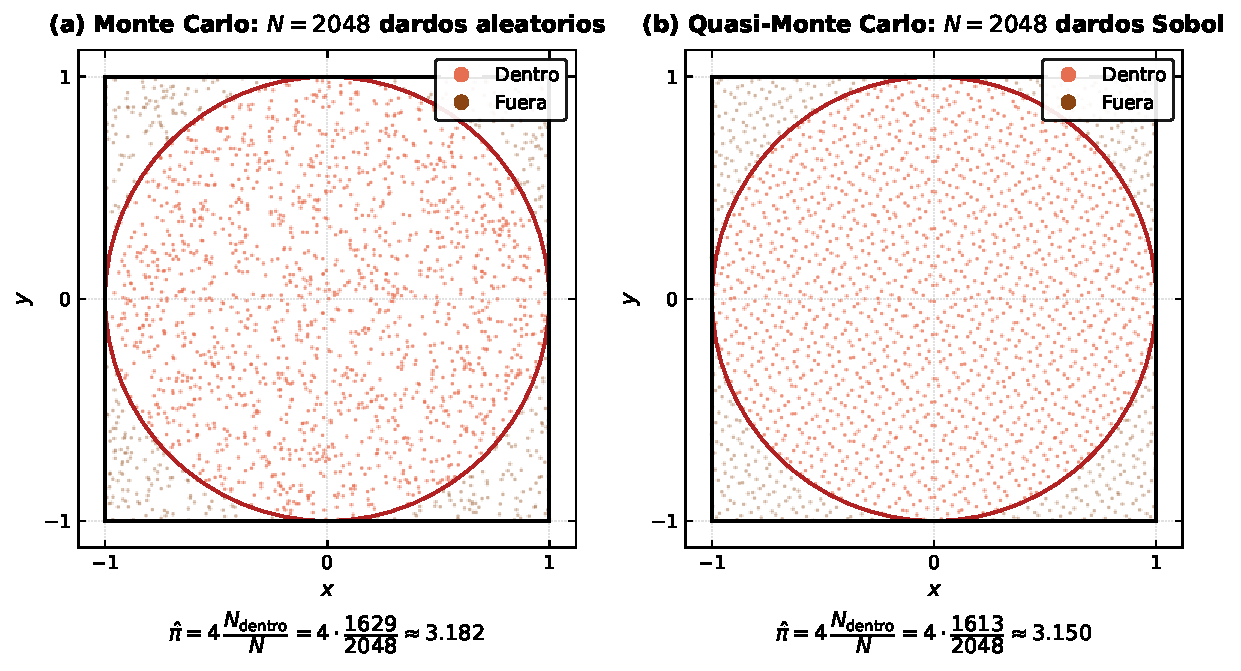
\includegraphics[width=1\linewidth]{Fig8.pdf}
    \caption{Estimación de $\pi$ mediante lanzamiento de dardos: comparación entre muestreo pseudoaleatorio (a) y secuencias de Sobol (b) con $N = 2048$, mostrando la distribución más uniforme de la QMC.}    
    \label{fig:pi_comparacion}
\end{figure}

Entre las distintas familias de secuencias de baja discrepancia, las secuencias de Sobol constituyen una de las alternativas más utilizadas gracias a su buena distribución en dimensiones moderadas y a la eficiencia de los algoritmos de generación disponibles \cite{sobol1967on}.

Sin embargo, su rendimiento disminuye conforme aumenta la dimensión efectiva del problema. En la simulación de procesos estocásticos, donde cada paso temporal introduce nuevas variables aleatorias, la dimensión puede alcanzar fácilmente varios cientos o miles de componentes, reduciendo parte de las ventajas asociadas a las secuencias de baja discrepancia.

Para mitigar este efecto se emplea la transformación \emph{Brownian Bridge}. Su idea fundamental consiste en modificar el orden de construcción del movimiento browniano. En lugar de generar cronológicamente todos los incrementos, primero se fija el valor del proceso en el instante final y posteriormente se reconstruyen los puntos intermedios mediante distribuciones normales condicionadas.

Esta reorganización permite asociar las primeras dimensiones de la secuencia de Sobol ---que poseen mejores propiedades de uniformidad--- a las componentes que explican una mayor proporción de la variabilidad de la trayectoria. Como consecuencia, la dimensión efectiva del problema disminuye y el rendimiento práctico del método cuasi-Monte Carlo mejora de forma significativa.

En el motor desarrollado, las variables uniformes generadas mediante Sobol se transforman en variables normales estándar mediante la función inversa de la distribución normal acumulada y, posteriormente, se reorganizan mediante el algoritmo Brownian Bridge antes de alimentar el esquema de discretización empleado por los distintos modelos financieros. Para preservar la independencia práctica entre bloques de simulación paralelos, cada hilo procesa un segmento diferente de la secuencia de Sobol.

\paragraph{Comparativa de las técnicas}

La Tabla \ref{tab:rng_comparison} resume las principales características de las estrategias consideradas. El generador Mersenne Twister se utiliza como referencia debido a su robustez y amplio uso en simulación científica. Las variables antitéticas proporcionan una reducción de varianza con un coste computacional muy reducido, mientras que la combinación de secuencias de Sobol y Brownian Bridge ofrece el mayor potencial de aceleración de la convergencia cuando la dimensión efectiva del problema permanece moderada.

\begin{table}[H]
\centering
\begin{tabular}{p{3cm}p{3.5cm}p{4cm}p{4cm}}
\toprule
Método & Fundamento & Ventajas & Limitaciones \\
\midrule
Mersenne Twister &
Generación pseudoaleatoria de alta calidad estadística. &
Robusto, eficiente y ampliamente validado. &
Convergencia Monte Carlo estándar. \\
\addlinespace
Variables antitéticas &
Construcción de estimadores negativamente correlacionados. &
Reduce la varianza con un coste prácticamente nulo. &
La mejora depende del problema considerado. \\
\addlinespace
Sobol + Brownian Bridge &
Secuencias de baja discrepancia combinadas con reducción de dimensión efectiva. &
Mayor uniformidad del muestreo y potencial aceleración de la convergencia. &
Mayor complejidad y eficacia dependiente de la dimensión efectiva del problema. \\
\bottomrule
\end{tabular}
\caption{Comparación de las técnicas de generación de trayectorias implementadas.}
\label{tab:rng_comparison}
\end{table}

\paragraph{Criterio de convergencia}

Otra estrategia para reducir el número de simulaciones consiste en incorporar un criterio de convergencia que determine de forma dinámica cuándo la estimación obtenida es suficientemente estable. De este modo, una vez que el resultado dejase de variar de forma significativa al añadir nuevas trayectorias, la simulación podría detenerse sin necesidad de alcanzar un número prefijado de iteraciones.

No obstante, con fines académicos, se ha optado por no implementar este mecanismo. En la mayoría de los experimentos realizados, mantener un control preciso sobre el número de simulaciones resulta fundamental para analizar y comprender el comportamiento del sistema, así como para comparar el rendimiento de las distintas optimizaciones bajo las mismas condiciones. De cara a una versión orientada a producción, sí sería recomendable incorporar un criterio de convergencia de este tipo, ya que permitiría evitar simulaciones innecesarias y mejorar la eficiencia del motor.

\subsubsection{Optimización computacional}

Si bien las técnicas de reducción de varianza disminuyen el número de simulaciones necesarias, el cumplimiento de las ventanas operativas en una sala de contratación exige que el software explote al máximo los recursos físicos del hardware. En esta sección se detallan las decisiones de ingeniería de software de bajo nivel implementadas en C++ para minimizar los cuellos de botella en la CPU y el bus de memoria.

\paragraph{Localidad de datos y optimización de caché (Evitando el Cache Missing)}

El rendimiento de un algoritmo masivo de Monte Carlo no suele verse limitado por la velocidad de cálculo aritmético de la CPU, sino por el tiempo que esta pasa esperando a que los datos se transfieran desde la memoria RAM. Las CPUs modernas mitigan esto mediante la memoria caché (L1, L2 y L3), que almacena líneas de datos contiguos de forma anticipada. Si el algoritmo intenta acceder a una posición de memoria que no está en la caché, se produce un fallo de caché (\textit{cache miss}), forzando una costosa lectura en la RAM que degrada el rendimiento de forma crítica.

En el diseño de este motor, la simulación de la cartera multifactorial se orquesta mediante una matriz bidimensional gestionada por la librería \texttt{Eigen}. En un eje de la matriz se estructuran los escenarios o simulaciones ($N$), mientras que en el otro se disponen las dimensiones temporales (pasos de discretización de los activos). Para limitar los fallos de caché debemos garantizar que el sentido en el que el bucle de ejecución recorre la matriz coincide exactamente con la forma en que los datos están indexados de forma física en la memoria.

Por defecto, la librería \texttt{Eigen} utiliza un almacenamiento por columnas (\textit{Column-Major}), siguiendo la convención habitual de bibliotecas algebraicas como BLAS o LAPACK (que por razones históricas, están basadas en Fortran). Sin embargo, la lógica de simulación de nuestro motor procesa de forma secuencial todas las trayectorias temporales de una simulación completa antes de saltar a la siguiente. Si se utilizase la configuración por defecto, cada paso de tiempo obligaría a la CPU a saltar de una columna a otra de la memoria física, provocando un *cache miss* sistemático en cada iteración del \textit{hot path}.

Para solucionar esto, se forzó al motor a trabajar bajo una estructura por filas invocado explícitamente mediante la plantilla \texttt{Eigen::Matrix<double, Dynamic, Dynamic, Eigen::RowMajor>}. Al alinear el diseño del almacenamiento físico de la memoria con el flujo de los bucles anidados del simulador, los hilos de la CPU encuentran los datos ya cargados de forma secuencial en las líneas de la caché L1/L2, reduciendo los tiempos de ejecución globales de forma drástica.

En la Fig. \ref{fig:comparativa_bucles} se muestra el ejemplo más sencillo que nos permite entender el impacto de este fenómeno (posteriormente en los resultados, analizaremos este efecto en nuestro motor).

\begin{figure}[htbp]
\centering
\begin{minipage}[t]{0.48\textwidth}
\centering
\small{\textbf{Variante 1: Almacenamiento por Columnas}}\\
\vspace{1mm}
% Forzamos \footnotesize específicamente para este bloque si no quieres cambiar el preámbulo global
\begin{lstlisting}[basicstyle=\ttfamily\footnotesize]
// colMajor(i,j) -> Salto en memoria
for (int r = 0; r < reps; ++r) {
    for (int i = 0; i < rows; ++i) {
        for (int j = 0; j < cols; ++j) {
            sum += colMajor(i, j);
        }
    }
}
\end{lstlisting}
\vspace{-2mm}
\footnotesize{\texttt{> Execution time: 30.28 s}\\ \textit{Menor localidad espacial (Cache misses).}}
\end{minipage}
\hfill 
\begin{minipage}[t]{0.48\textwidth}
\centering
\small{\textbf{Variante 2: Almacenamiento por Filas}}\\
\vspace{1mm}
\begin{lstlisting}[basicstyle=\ttfamily\footnotesize]
// rowMajor(i,j) -> Acceso secuencial
for (int r = 0; r < reps; ++r) {
    for (int i = 0; i < rows; ++i) {
        for (int j = 0; j < cols; ++j) {
            sum += rowMajor(i, j);
        }
    }
}
\end{lstlisting}
\vspace{-2mm}
\footnotesize{\texttt{> Execution time: 2.16 s}\\ \textit{Alta localidad espacial (Cache hits).}}
\end{minipage}
\caption{Impacto del orden de almacenamiento en memoria (\textit{column-major} vs. \textit{row-major}) en el rendimiento de bucles anidados utilizando \texttt{Eigen}. El experimento evalúa la misma matriz cuadrada de dimensiones $4096 \times 4096$ ejecutando \texttt{reps = 50} iteraciones. La variante optimizada alcanza un factor de aceleración (\textit{speedup}) de $\approx 14$.}
\label{fig:comparativa_bucles}
\end{figure}

\paragraph{Gestión eficiente de memoria y vectorización SIMD}

Se diferencia entre la generación completa de trayectorias y el cálculo directo del valor terminal. Durante la ejecución habitual del motor, los activos utilizan el método \texttt{simulateFinalValue()}, que devuelve únicamente el valor necesario para el cálculo del PnL. En consecuencia, las opciones europeas calculan directamente el precio final del subyacente sin almacenar valores intermedios, mientras que las opciones barrera evalúan la condición de activación mediante un recorrido secuencial y un indicador lógico de estado.

La materialización completa de trayectorias mediante \texttt{generatePath()} queda reservada a tareas de validación, depuración y análisis, reduciendo significativamente las asignaciones dinámicas en la ruta crítica de ejecución.

Además, dentro del bucle crítico de simulación (donde se ejecutan las millones de iteraciones), realizar llamadas al sistema para reservar memoria dinámica —como el uso descuidado de \texttt{new}, \texttt{std::vector::push\_back} o redimensionamientos dinámicos— es un error fatal de rendimiento que fragmenta la memoria y bloquea los hilos de ejecución.

Para evitar este cuello de botella, el software implementa una estrategia de \textbf{preasignación de memoria contigua} (\textit{flat memory structure}). Antes de arrancar la primera simulación, el motor calcula el tamaño exacto que requerirá toda la matriz de resultados basándose en los parámetros inyectados por \texttt{SimConfig}. Toda la memoria necesaria se reserva de golpe en un único bloque contiguo. Durante la simulación, el motor simplemente sobreescribe de forma directa las posiciones de memoria ya existentes mediante punteros y operaciones de indexación rápida.

Esta disposición contigua de la memoria, sumada al uso de las estructuras optimizadas de \texttt{Eigen}, permite que el compilador active de forma automática la \textbf{vectorización por hardware} (\textit{Single Instruction Multiple Data}, SIMD). Gracias a esto, la CPU no procesa las trayectorias de los activos de una en una, sino que empaqueta múltiples valores en registros vectoriales anchos (AVX-2 o AVX-512) y ejecuta la dinámica matemática sobre 4 u 8 activos de manera simultánea en un único ciclo de reloj. %NO ME TERMINA DE GUSTAR ESTO LA VERDAD...

\paragraph{Paralelismo y concurrencia a nivel de proceso}

La simulación Monte Carlo presenta una estructura naturalmente paralelizable, ya que cada trayectoria puede generarse y evaluarse de forma independiente. Esta característica resulta especialmente relevante en aplicaciones de gestión de riesgos, donde la precisión de métricas depende directamente del número de escenarios simulados, como ya hemos visto anteriormente.

Es por esto que el motor desarrollado distribuye las simulaciones mediante una estrategia de partición por \emph{batches}. El número total de trayectorias se divide entre varios trabajadores independientes lanzados mediante \texttt{std::async}, donde cada hilo ejecuta una instancia de \texttt{runBatchImpl()} y devuelve un vector local de valores de PnL. Una vez finalizadas todas las tareas, el hilo principal agrega los resultados y construye la distribución empírica utilizada para el cálculo de las métricas de riesgo.

La granularidad elegida es deliberadamente gruesa, ya que cada trabajador procesa miles de simulaciones antes de sincronizarse con el resto. Asimismo, se evita cualquier forma de paralelismo anidado dentro de \texttt{runBatchImpl()}, por lo que no se emplean algoritmos paralelos adicionales sobre los bucles de activos o pasos temporales. Esta decisión reduce la complejidad de sincronización y evita fenómenos de \emph{oversubscription}, donde el número de tareas activas supera los recursos físicos disponibles.

\subparagraph{Escalabilidad del motor}
Desde un punto de vista teórico, la escalabilidad un sistema puede analizarse inicialmente mediante la Ley de Amdahl \cite{amdahl1967validity}. Esta ley se basa en que el tiempo total de ejecución de un programa se puede dividir en el tiempo asociado a procesos no paralelizables (secuenciales) y el tiempo asociado a procesos paralelizables. Esto se ve bien en la Figura~\ref{fig:amdahl_montecarlo}.

\begin{figure}[H]
\centering
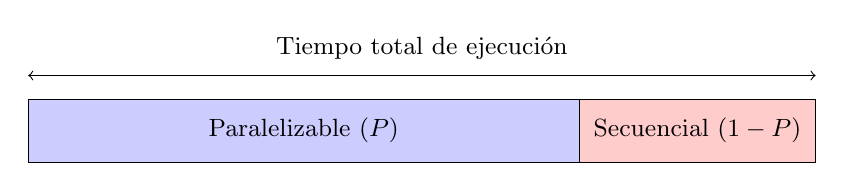
\begin{tikzpicture}[font=\small]
\draw[fill=blue!20] (0,0) rectangle (7,0.8);
\draw[fill=red!20] (7,0) rectangle (10,0.8);

\node at (3.5,0.4) {Paralelizable ($P$)};
\node at (8.5,0.4) {Secuencial ($1-P$)};

\draw[<->] (0,1.1) -- (10,1.1);
\node at (5,1.45) {Tiempo total de ejecución};
\end{tikzpicture}
\caption{Descomposición conceptual del tiempo de ejecución utilizada en los modelos de escalabilidad.}
\label{fig:amdahl_montecarlo}
\end{figure}
Asumiendo esto, si \(P\) representa la fracción paralelizable del algoritmo y \(k\) el número de procesadores empleados, el \emph{speedup} teórico que Amdahl dedujo viene dado por

\begin{equation}
S(k)=
\frac{1}
{(1-P)+\frac{P}{k}}.
\label{eq:amdahl}
\end{equation}

La ecuación (\ref{eq:amdahl}) pone de manifiesto que incluso una pequeña componente secuencial limita la aceleración máxima alcanzable. No obstante, este modelo asume procesadores independientes y ausencia de costes de coordinación, hipótesis que rara vez se cumplen en arquitecturas modernas.

Por este motivo, el análisis de escalabilidad se puede complementar mediante la \emph{Universal Scalability Law} (USL) de Gunther \cite{gunther1993simple},

\begin{equation}
S(k)
=
\frac{k}
{1+\alpha(k-1)+\beta k(k-1)},
\label{eq:usl}
\end{equation}
donde \(\alpha\) modeliza la contención sobre recursos compartidos y \(\beta\) representa los costes asociados a sincronización y coherencia entre tareas concurrentes.

Asimismo, los procesadores actuales incorporan tecnologías de \emph{Simultaneous Multithreading} (SMT) \cite{tullsen1995simultaneous}, en las que varios hilos lógicos comparten un mismo núcleo físico. Como consecuencia, la capacidad efectiva de cómputo deja de crecer linealmente con el número de hilos disponibles. Dejando los detalles en el Apéndice B, se puede tratar de generalizar la USL al uso de SMT \cite{hill2008amdahl}, llegando a la siguiente expresión:

\begin{equation}
S(k) = 
\begin{cases} 
\frac{1}{(1 - P) + \frac{P}{k} + \beta(k - 1)} & \text{si } k \le N \\[1.5em]
\frac{1}{(1 - P) + \frac{P}{k \cdot c} + \beta(k - 1)} & \text{si } N < k \le 2N 
\end{cases}
\label{eq:amdahl_best}
\end{equation}
donde $c$ cuantifica el rendimiento relativo del segundo hilo lógico respecto al de un núcleo físico dedicado. Si no existiese SMT y el paralelismo se obtuviese mediante núcleos físicos independientes, $c=1$. Cuando dos hilos lógicos comparten un mismo núcleo físico, el segundo hilo no equivale a un núcleo adicional completo, sino que aporta únicamente una fracción de su capacidad de cómputo, por lo que $c<1$. Este factor se calibrará experimentalmente para la arquitectura considerada, tomando como referencia el rendimiento en operaciones de FPU.

Los benchmarks desarrollados en este proyecto permiten contrastar experimentalmente estas predicciones teóricas, evaluando la evolución del rendimiento al incrementar el número de cores tanto en escenarios reducidos como en carteras de mayor dimensión.


% =========================================================================
% CAPÍTULO 6: ANÁLISIS DE RESULTADOS EMPÍRICOS
% =========================================================================

\section{Análisis de Resultados Empíricos}

%TEST QUE QUIERO HACER:
%- Tests matemáticos
%Test de convergencia. Ver cómo una misma cartera, con los tres métodos de generación de números, convergen mejor a los valores reales. Este test se presentará tanto para VaR como para ES y quiero también hacer un análisis cuantitativo de la varianza real, para el cual debo incluir un apéndice explicando la obtención de dichos errores.
%También estaría bien ver cómo escala esto con la cantidad de activos que tenemos y con la dinámica de Hull-White activa. En teoría, como tenemos tres dimensiones $N_{activos}\times N_{paths\_activo}\times N_{simulaciones}$, por cada simulación que disminuyamos, deberíamos ver una disminución x.

%Test de caché. Cambiamos las matrices de Eigen, por col y comparamos tiempos de ejecución para N simulaciones. Aquí, por simplificar, no pondría una gran cartera.

%Test de escalabilidad. Aquí sí que vamos a por Amdahl a saco. Para ello, vamos a sacar dos gráficas. Una de ellas, con la cartera base, que y vemos qué tan bien paraleliza. La siguiente, analizaremos como mejora o empeora la situación cuando incorporamos nuevos activos.

Este capítulo expone la evaluación empírica del motor de cálculo de riesgo multifactorial desarrollado. El objetivo es contrastar cuantitativamente las hipótesis de diseño planteadas en los capítulos previos ---en particular, los criterios de aceptación \texttt{CA-01}--\texttt{CA-07} de la Tabla~\ref{tab:criterios_aceptacion}---, dividiendo el análisis en dos dimensiones críticas: la eficiencia matemática (calidad y velocidad de convergencia de las métricas de riesgo) y la eficiencia computacional (impacto de las optimizaciones de bajo nivel y escalabilidad del paralelismo en C++).

\subsection{Diseño de experimentos y entorno de pruebas}

Para garantizar la replicabilidad científica de los resultados, todas las pruebas se han ejecutado bajo un entorno de hardware controlado, cuyas especificaciones técnicas se detallan en la Tabla \ref{tab:hardware}.

\begin{table}[H]
    \centering
    \begin{tabular}{ll}
        \hline
        \textbf{Componente} & \textbf{Especificación Técnica} \\ \hline
        Arquitectura de CPU & AMD Ryzen 7 5700U with Radeon Graphics \\
        Núcleos Físicos / Hilos Lógicos & 8 núcleos / 16 hilos \\
        Frecuencia de Reloj Base & 1.8 GHz \\
        Memoria Caché L1 / L2 / L3 & 512 KB / 4 MB / 8 MB \\
        Memoria RAM Disponible & 8 GB DDR4 @ 3200 MHz \\
        Compilador y Flags de Optimización & \texttt{g++ 15.2.0 / -O3 -march=native} \\ \hline
    \end{tabular}
    \caption{Especificaciones del entorno de hardware de ejecución.}
    \label{tab:hardware}
\end{table}

\paragraph{Cartera de referencia.}
Todos los resultados se obtienen sobre una cartera sintética multi-activo completamente especificada, utilizada como escenario \emph{benchmark} común para los experimentos de riesgo.

\begin{table}[h]
\centering
\small
\begin{tabular}{ll}
\toprule
\multicolumn{2}{l}{\textbf{Posiciones de la cartera}} \\
\midrule
1. GBMAsset & cantidad $q=50$; $S_0=100$; $\mu=0{,}02$; $\sigma=0{,}20$ \\
2. EuropeanOption (Call) & $q=400$; prima $=12$; $S_0=100$; $K=105$; $\mu=0{,}02$; $\sigma=0{,}25$ \\
3. Up-and-out Call & $q=500$; prima $=8$; $S_0=100$; $K=100$; $B=130$; $\mu=0{,}02$; $\sigma=0{,}28$ \\
& Knock-out si $S\ge B$ en algún paso de monitorización discreta \\
4. CouponBond (Hull--White) & $q=5$; nominal $=1000$; cupón anual $c=3\%$; $T_m=5$ años \\
\midrule
Valor inicial cartera & $V_0 \approx 18\,794{,}5$ \\
\midrule
\multicolumn{2}{l}{\textbf{Hull--White}} \\
\midrule
Reversión a la media & $a=0{,}05$ \\
Volatilidad del tipo corto & $\sigma_r=0{,}01$ \\
Curva zero inicial & $(0{,}5,2{,}0\%),\ (1,2{,}2\%),\ (2,2{,}5\%),\ (5,3{,}0\%),\ (10,3{,}2\%)$ \\
Tasa corta inicial & Forward implícito de la curva en $t=0$ \\
Acoplamiento & Drift GBM $= r_t+\mu$ \\
Descuento & Integración trapezoidal de $r_t$ sobre la trayectoria \\
\midrule
\multicolumn{2}{l}{\textbf{Correlación (factores: Equity, EuroCall, BarrierCall, Bond, Rate)}} \\
\midrule
$\mathbf{R}$ &
$\begin{bmatrix}
1.00 & 0.80 & 0.60 & -0.20 & 0.25 \\
0.80 & 1.00 & 0.55 & -0.15 & 0.22 \\
0.60 & 0.55 & 1.00 & -0.12 & 0.18 \\
-0.20 & -0.15 & -0.12 & 1.00 & 0.45 \\
0.25 & 0.22 & 0.18 & 0.45 & 1.00
\end{bmatrix}$ \\
Dimensión estocástica & $5$ factores $\times 50$ pasos $=250$ normales estándar por trayectoria \\
\midrule
\multicolumn{2}{l}{\textbf{Parámetros de Monte Carlo}} \\
\midrule
A concretar en cada test \\
\midrule
\multicolumn{2}{l}{\textbf{Dinámica}} \\
\midrule
Equity y opciones &
$S_{i+1}=S_i\exp\!\left((r_i+\mu-\tfrac12\sigma^2)\Delta t+\sigma\sqrt{\Delta t}\,Z_i\right)$ \\
Payoff call europea & $\max(S_T-K,0)$ \\
Payoff barrera & $0$ si hay knock-out; en otro caso $\max(S_T-K,0)$ \\
\bottomrule
\end{tabular}
\caption{Especificaciones del escenario \texttt{benchmark1}.}
\end{table}

\subsection{Evaluación de la dimensión matemática: Reducción de varianza}

En esta sección se analiza cómo la integración de las secuencias de baja discrepancia de Sobol combinadas con el Puente Browniano y las variables antitéticas acelera la convergencia del \textit{Value at Risk} ($\text{VaR}_{0.99}$) y del \textit{Expected Shortfall} ($\text{ES}_{0.975}$) frente al método de Monte Carlo clásico (pseudoaleatorio puro).

\subsubsection{Velocidad de convergencia}

La Figura~\ref{fig:convergencia_var_es} resume la convergencia del $\text{VaR}_{99\%}$ y del $\text{ES}_{97{,}5\%}$ en la cartera base (\texttt{benchmark1} con modelo Hull--White) al aumentar el número de simulaciones $N$ desde $2^8$ hasta $2^{17}$. Se comparan tres configuraciones del generador de números aleatorios: Mersenne Twister (MC clásico), variables antitéticas y secuencia de Sobol (con puente browniano en la construcción de trayectorias). La figura combina, para cada métrica, la evolución del estimador con su banda de incertidumbre $\pm\,\text{SE}$ (paneles superiores) y el decaimiento del error relativo $\text{SE}/|\hat{\theta}|$ en escala log--log (paneles inferiores), donde se ajusta una ley de potencia $\propto N^{\alpha}$ y se incluye la referencia teórica $\mathcal{O}(N^{-1/2})$ del Monte Carlo estándar.

\begin{figure}[H]
    \centering
    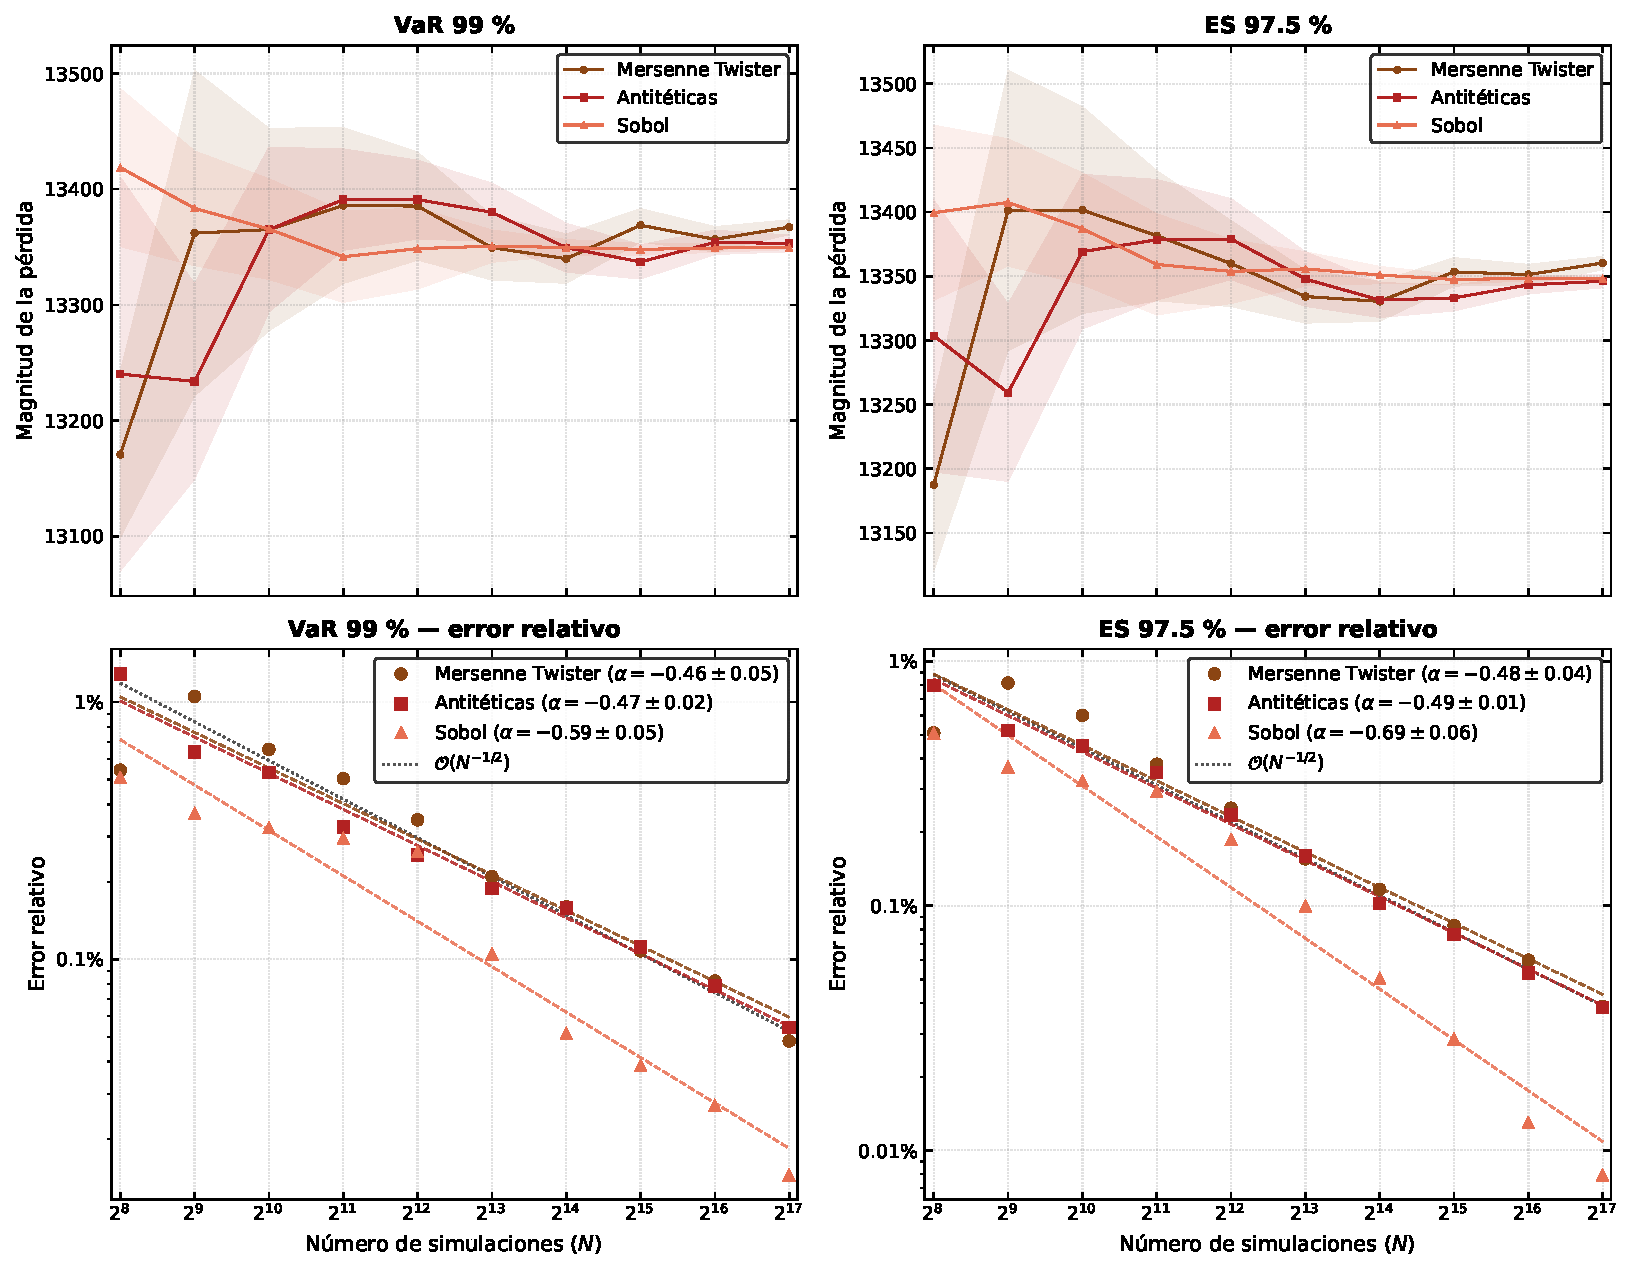
\includegraphics[width=1\textwidth]{Fig9.pdf}
    \caption{Convergencia del $\text{VaR}_{99\%}$ y del $\text{ES}_{97{,}5\%}$ frente a $N$, con Mersenne Twister, variables antitéticas y Sobol. En los paneles superiores se muestra la magnitud de la pérdida con bandas $\pm\,\text{SE}$; en los inferiores, el error relativo en escala log--log con el ajuste $\alpha$ y la referencia $\mathcal{O}(N^{-1/2})$.}
    \label{fig:convergencia_var_es}
\end{figure}

\paragraph{Estabilidad del estimador}
En los paneles superiores, las tres configuraciones convergen hacia una magnitud de pérdida común del orden de $13\,350$--$13\,370$ para el $\text{VaR}_{99\%}$ y de $13\,340$--$13\,360$ para el $\text{ES}_{97{,}5\%}$, lo que indica que las diferencias entre generadores afectan sobre todo a la \emph{precisión} del estimador y no a un sesgo sistemático apreciable. No obstante, el camino hacia ese valor difiere claramente: Mersenne Twister presenta oscilaciones más pronunciadas para $N$ pequeño (p.\,ej., en el $\text{VaR}_{99\%}$ el estimador varía más de $200$ unidades entre $N=256$ y $N=4096$), y sus bandas de error permanecen más anchas durante buena parte del recorrido. Con $N=2048$, la incertidumbre del $\text{VaR}_{99\%}$ bajo MT es de $\pm 67$ frente a $\pm 40$ con Sobol, es decir, una banda casi un $40\%$ más estrecha con el mismo número de escenarios. Sobol, en cambio, describe una trayectoria más regular desde el primer punto y estrecha sus bandas con mayor rapidez.

\paragraph{Tasa de convergencia del error.}
Los paneles inferiores cuantifican este comportamiento. Para MT y antitéticas, el exponente ajustado se sitúa en torno a $\alpha \approx -0{,}46$ ($\text{VaR}_{99\%}$) y $\alpha \approx -0{,}48$--$-0{,}49$ ($\text{ES}_{97{,}5\%}$), coherente con la pendiente de referencia $-1/2$ del Monte Carlo clásico. Sobol exhibe un decaimiento sistemáticamente más rápido: $\alpha \approx -0{,}59$ en el $\text{VaR}_{99\%}$ y $\alpha \approx -0{,}69$ en el $\text{ES}_{97{,}5\%}$, quedando en ambos casos por debajo de la recta $\mathcal{O}(N^{-1/2})$. La ventaja es especialmente marcada en el $\text{ES}_{97{,}5\%}$, métrica que depende de la media en la cola de la distribución y, por tanto, exige un muestreo más denso en la región extrema.

\paragraph{Implicaciones prácticas}
Al final del barrido ($N=2^{17}$), el error relativo del $\text{VaR}_{99\%}$ cae al $0{,}048\%$ con MT y al $0{,}015\%$ con Sobol; en el $\text{ES}_{97{,}5\%}$, de $0{,}039\%$ a $0{,}008\%$. Equivale a una reducción del error de entre tres y cinco veces a igual número de simulaciones, o —visto al revés— a alcanzar con $N \approx 2^{15}$ un nivel de precisión relativa que MT solo consigue cerca de $2^{17}$. Las variables antitéticas no mejoran de forma consistente respecto a MT en este escenario (si bien el coste computacional sí es menor al generar la mitad de variables aleatorias): en algunos puntos del barrido (p.\,ej., $N=256$) incrementan incluso la incertidumbre del $\text{VaR}_{99\%}$, probablemente por la correlación inducida entre pares antitéticos en una cartera multiactivo con estructura de colas no simétrica.

En conjunto, la figura muestra que la elección del generador no es un detalle de implementación secundario: condiciona directamente cuántas simulaciones hacen falta para que las métricas de cola dejen de fluctuar y puedan interpretarse con la estabilidad que exige un uso cuantitativo del motor de riesgo.

\subsection{Evaluación de la dimensión computacional: Alto rendimiento (HPC)}

Esta sección evalúa el impacto en el tiempo de ejecución puro provocado por las optimizaciones de bajo nivel en C++ implementadas en el Capítulo 5.

\subsubsection{Impacto de la localidad de datos (Row-Major vs. Col-Major)}

Con objeto de cuantificar el impacto práctico de la disposición en memoria de la matriz de choques sobre el rendimiento del motor, se realizó un experimento de contraste entre la configuración de producción (\texttt{RowMajor}) y una variante contrafactual equivalente basada en \texttt{ColMajor}. El objetivo no es reevaluar la decisión de diseño ya justificada en la sección de implementación, sino medir empíricamente su efecto sobre el tiempo de ejecución.

Para evaluar este efecto, vamos a ir ampliando el tamaño de la cartera para hacer que las matrices sean cada vez más pesadas. Para ello, crearemos réplicas independientes de la cartera base multi-activo (\texttt{benchmark1}), es decir, multiplicaremos la cantidad de cada activo de nuestra cartera de referencia. La matriz de correlación se construye por bloques, replicando la estructura intra-réplica y aplicando un factor de atenuación de 0,75 a las correlaciones entre réplicas distintas.

El experimento escala el número de réplicas en el conjunto
\[
\{16,32,64,128,256,512,1024,2048\},
\]
lo que genera carteras entre 64 y 8192 activos. El horizonte temporal permanece fijo en un año con $S=50$ pasos, de forma que el crecimiento del problema se produce exclusivamente a través de la dimensión de factores. Todas las ejecuciones se hacen con un solo core (para evitar efectos provenientes del paralelismo), generador \texttt{std::mt19937} y exactamente la misma secuencia aleatoria para cada par RowMajor/ColMajor. La métrica de comparación es

\[
\text{Speedup}=
\frac{\text{Time}_{\mathrm{ColMajor}}}
     {\text{Time}_{\mathrm{RowMajor}}},
\]
de modo que valores superiores a uno indican una ventaja para la implementación RowMajor.

\begin{figure}[H]
    \centering
    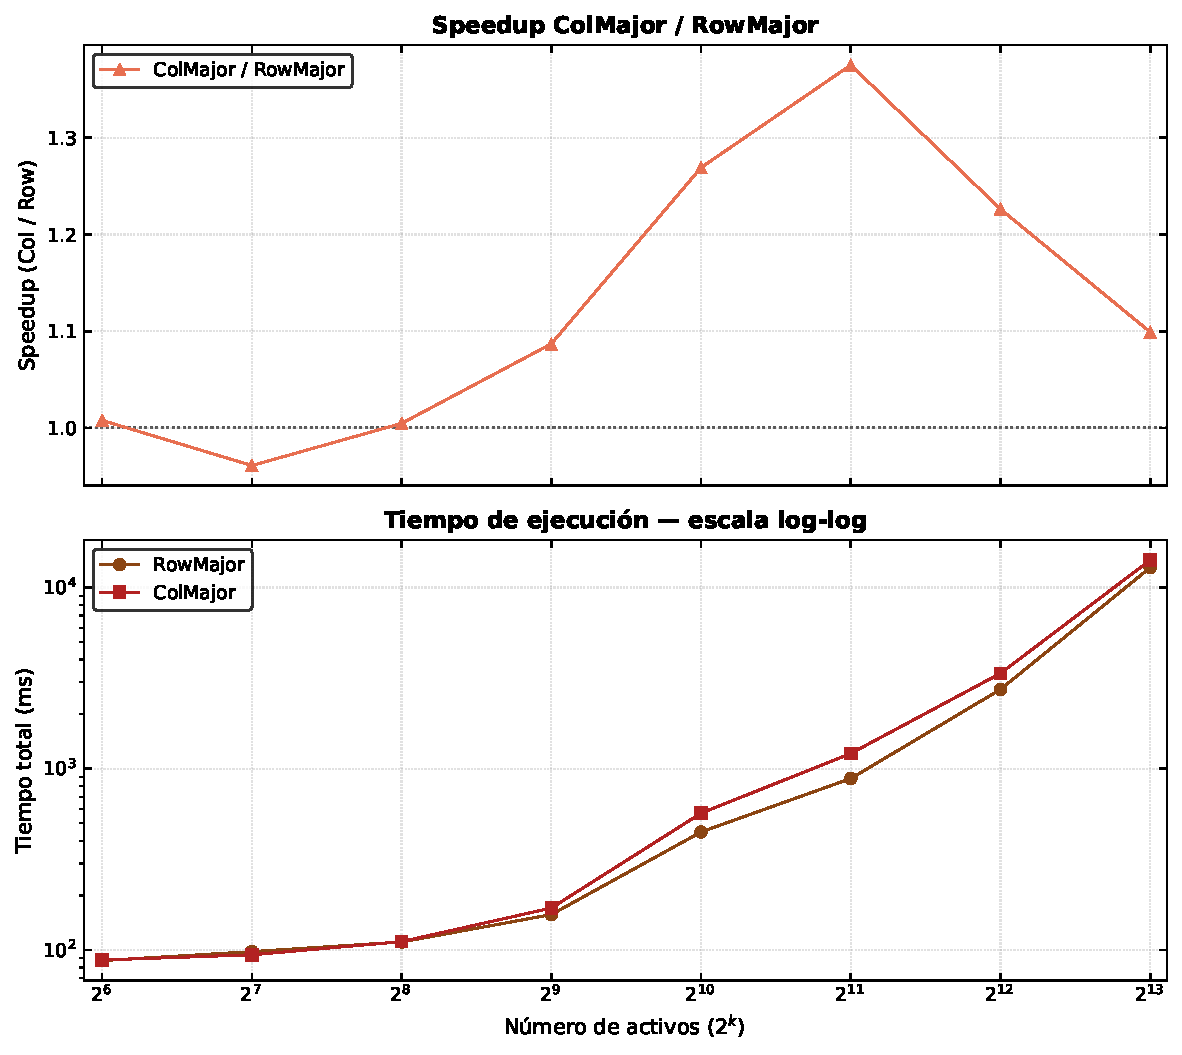
\includegraphics[width=0.8\textwidth]{Fig10.pdf}
    \caption{Speedup de ColMajor frente a RowMajor y tiempos de ejecución en función del número de activos para benchmark1 replicada (cada réplica añade 4 activos: GBM, call europea, opción barrera y bono HW). Panel superior: ratio de tiempos ColMajor/RowMajor (valores > 1 indican ventaja de RowMajor); línea punteada en 1. Panel inferior: tiempo total en escala log–log para ambos layouts. Eje horizontal en potencias de 2 ($64 \ldots 8,192$ activos, equivalente a $16 \ldots 2,048$ réplicas). Configuración: $T=1$ año, 50 pasos temporales, Mersenne Twister (semilla fija), 2 núcleos, $N$ adaptativo por escala; el VaR al 99 \% coincide en todos los puntos.}
    \label{fig:benchmark_layout_speedup_activos}
\end{figure}

En la Figura~\ref{fig:benchmark_layout_speedup_activos} se muestra la evolución del \emph{speedup} y los tiempos absolutos en escala logarítmica.
El comportamiento de la curva de \emph{speedup} puede interpretarse a partir de la geometría de la matriz de shocks $Z \in \mathbb{R}^{F \times S}$ ($F$ factores de riesgo, $S$ pasos temporales) y del patrón de acceso del motor: tras generar normales independientes y aplicar la correlación mediante $Z_{\mathrm{corr}} = L Z_{\mathrm{indep}}$ (descomposición de Cholesky de la matriz de correlación), la revaloración de la cartera consume \emph{filas} completas de $Z_{\mathrm{corr}}$---una por activo---en \texttt{Portfolio::simulatePathPnL}.
Con $S=50$ fijo y $F$ creciente al replicar la cartera \texttt{benchmark1}, RowMajor almacena cada trayectoria de factor en memoria contigua, alineándose con ese patrón dominante; ColMajor optimiza, en cambio, el relleno columna a columna, pero penaliza las lecturas fila a fila posteriores.

Tres regímenes pueden distinguirse en la figura.
En carteras pequeñas ($64$--$512$ activos), el \emph{speedup} permanece en torno a $1$: la huella de $Z$ es reducida y ambos layouts permanecen en caché, de modo que la diferencia de layout es del orden del ruido experimental.
A partir de $1\,024$ activos la brecha se amplía hasta un máximo de $1{,}36$ en $2\,048$ activos ($958$\,ms frente a $1\,299$\,ms), cuando el producto matricial $L Z_{\mathrm{indep}}$ ---de coste $\mathcal{O}(F^2 S)$--- domina el tiempo de ejecución.
Por último, entre $4\,096$ y $8\,192$ activos el \emph{speedup} desciende hasta $1{,}11$: ambos layouts comparten cuellos de botella de memoria (\texttt{memcpy}, \texttt{free\_base}, empaquetado previo al GEMM) y la ventaja relativa de RowMajor se comprime, aunque no desaparece.

Para corroborar la interpretación, se perfiló \texttt{integration\_tests.exe} con \emph{Intel VTune Profiler} \cite{intel_vtune_2026} (vista \emph{Bottom-up}, un hilo, misma semilla y parámetros que en el benchmark).
La escala de cartera se construye replicando \texttt{benchmark1} ($4$ activos por réplica); el punto de máximo \emph{speedup} corresponde a $512$ réplicas ($2\,048$ activos).
La Figura~\ref{fig:vtune_layout} reproduce las capturas directas del profiler en esa configuración.
En ColMajor, los \emph{hotspots} principales son instrucciones de almacenamiento y carga vectorial (\texttt{\_mm256\_store\_pd} $\approx 214$\,ms, \texttt{\_mm256\_loadu\_pd} $\approx 78$\,ms), seguidas del mapeo interno de Eigen (\texttt{blas\_data\_mapper} $\approx 171$\,ms) y \texttt{free\_base} ($\approx 66$\,ms): el tiempo efectivo se concentra en mover datos más que en aritmética (\texttt{\_mm256\_fmadd\_pd} $\approx 48$\,ms).
En RowMajor, bajo idéntica carga, dominan las operaciones \texttt{\_mm256\_fmadd\_pd} ($\approx 118$\,ms), el empaquetado del operando derecho del GEMM (\texttt{gemm\_pack\_rhs} $\approx 82$\,ms) y los \emph{kernels} \texttt{gebp\_kernel} ($\approx 63{+}42$\,ms): el mismo producto $L Z_{\mathrm{indep}}$ se ejecuta con una fracción mayor de trabajo aritmético vectorial y menos penalización en \emph{store}/\emph{load} aislados.
Este contraste es coherente con la ratio $1{,}36$ de la Figura~\ref{fig:benchmark_layout_speedup_activos}.

\begin{figure}[H]
    \centering
    \begin{subfigure}[t]{0.49\textwidth}
        \centering
        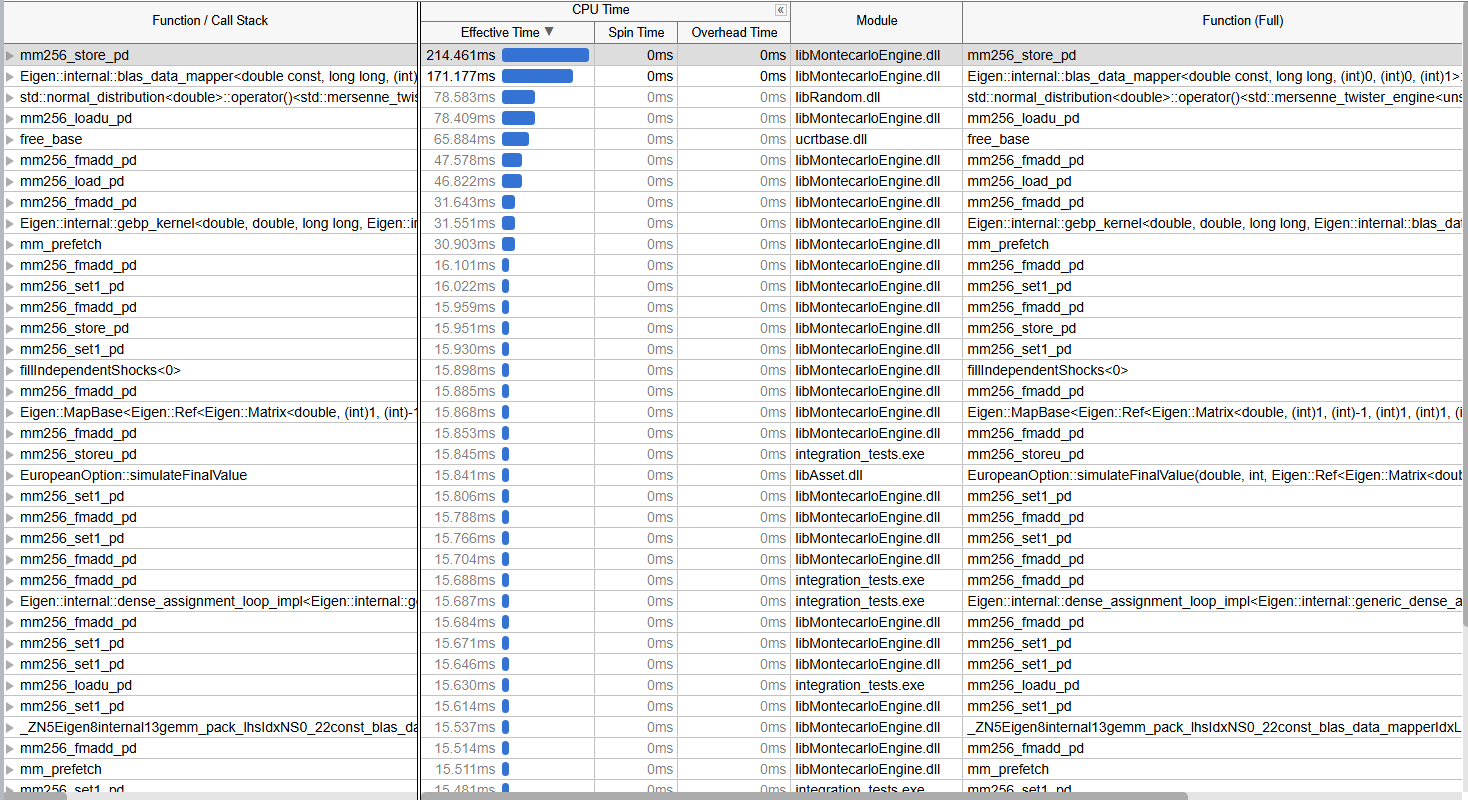
\includegraphics[width=\textwidth]{Fig11.png}
        \caption{ColMajor ($512$ réplicas, $2\,048$ activos).}
        \label{fig:vtune_layout_col}
    \end{subfigure}
    \hfill
    \begin{subfigure}[t]{0.48\textwidth}
        \centering
        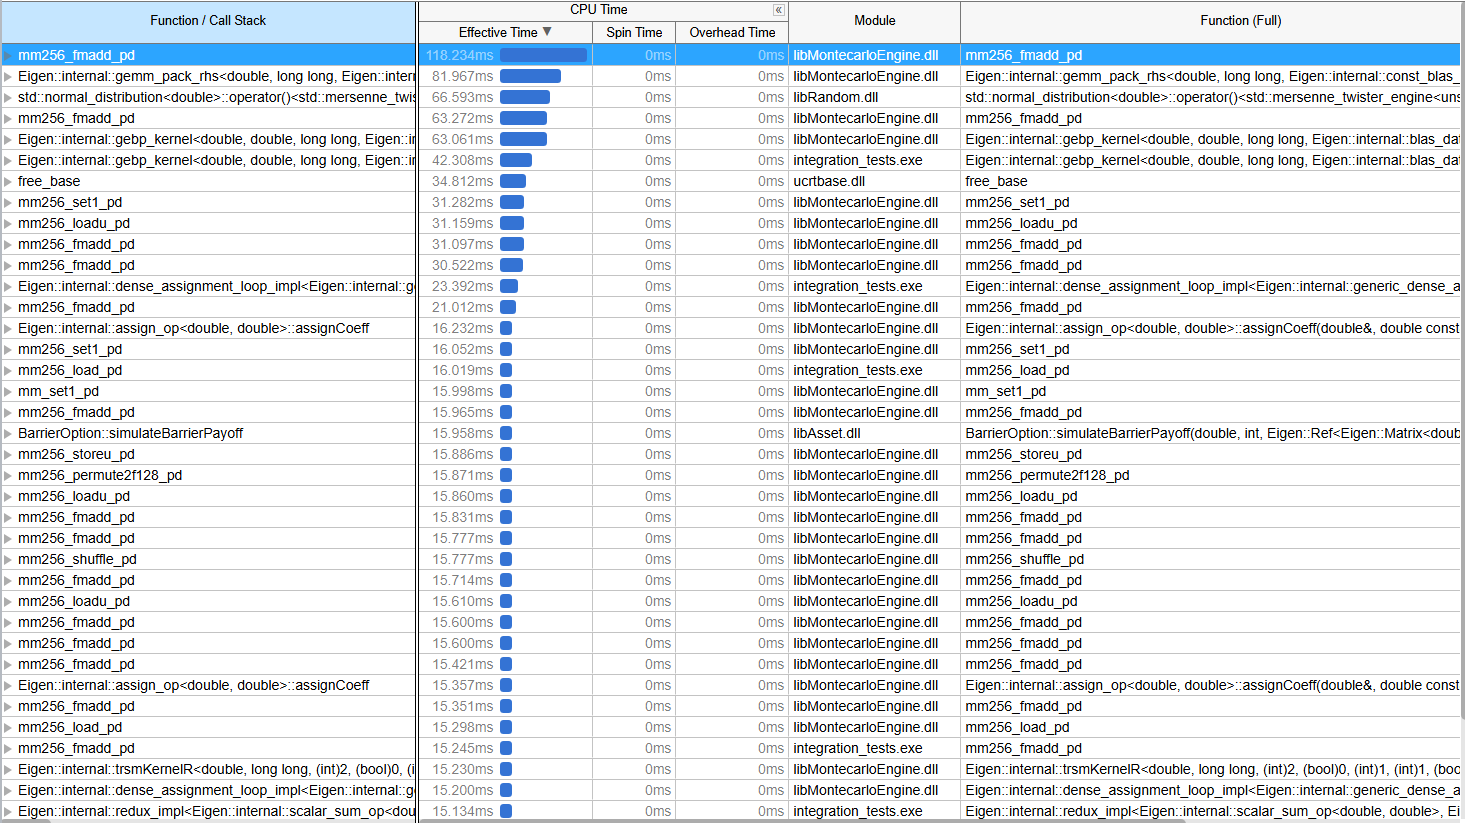
\includegraphics[width=\textwidth]{Fig12.png}
        \caption{RowMajor ($512$ réplicas, $2\,048$ activos).}
        \label{fig:vtune_layout_row}
    \end{subfigure}
    \caption{Intel VTune Profiler (\emph{Bottom-up}, tiempo efectivo de CPU) en el máximo \emph{speedup} ColMajor/RowMajor ($512$ réplicas, $2\,048$ activos; $N=50$, $T=1$ año, $50$ pasos).}
    \label{fig:vtune_layout}
\end{figure}

Al extender el análisis a $64$, $512$ y $2\,048$ réplicas ($256$, $2\,048$ y $8\,192$ activos), la Figura~\ref{fig:vtune_layout_escala} resume la repartición agregada del tiempo de CPU entre acceso o gestión de memoria y cálculo (aritmética vectorial y generación aleatoria), cuantificada a partir de las mismas sesiones de profiling.
En el máximo de \emph{speedup} ($512$ réplicas), RowMajor dedica una fracción sensiblemente mayor al cálculo ($\approx 61\,\%$ frente a $\approx 39\,\%$ en ColMajor), coherente con las capturas de la Figura~\ref{fig:vtune_layout}.
A $2\,048$ réplicas ($8\,192$ activos), la componente de memoria crece en \emph{ambos} layouts ($\approx 76\,\%$ ColMajor, $\approx 60\,\%$ RowMajor), lo que explica la convergencia de los tiempos absolutos en el panel inferior de la Figura~\ref{fig:benchmark_layout_speedup_activos} y la compresión del \emph{speedup} hacia la unidad.

\begin{figure}[H]
    \centering
    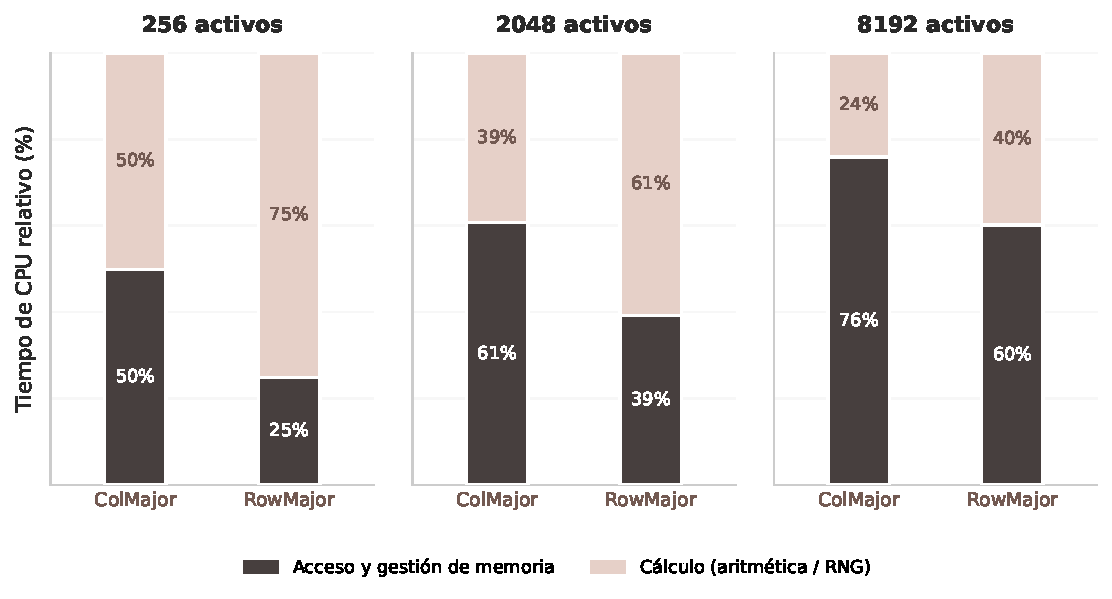
\includegraphics[width=0.92\textwidth]{Fig13.pdf}
    \caption{Repartición agregada del tiempo de CPU (memoria vs.\ cálculo) según VTune en $64$, $512$ y $2\,048$ réplicas ($256$, $2\,048$ y $8\,192$ activos). Complementa las capturas de la Figura~\ref{fig:vtune_layout}.}
    \label{fig:vtune_layout_escala}
\end{figure}


\subsubsection{Escalabilidad del paralelismo multihilo}

Para analizar el comportamiento de la concurrencia nativa sin estado compartido, se lanzó el benchmark base sobre la cartera \texttt{benchmark1} ($4$ activos, $50$ pasos temporales, Mersenne Twister, semilla fija) con $N = 100\,000$ simulaciones, variando de forma progresiva el número de hilos de ejecución activos del sistema ($k = 1, \ldots, K$, con $K = \texttt{hardware\_concurrency()}$).
Cada punto agrega $1\,000$ mediciones independientes tras un calentamiento de $25$ iteraciones.
Los resultados de escalabilidad se presentan en la Figura~\ref{fig:paralelismo_speedup}.

\begin{figure}[H]
    \centering
    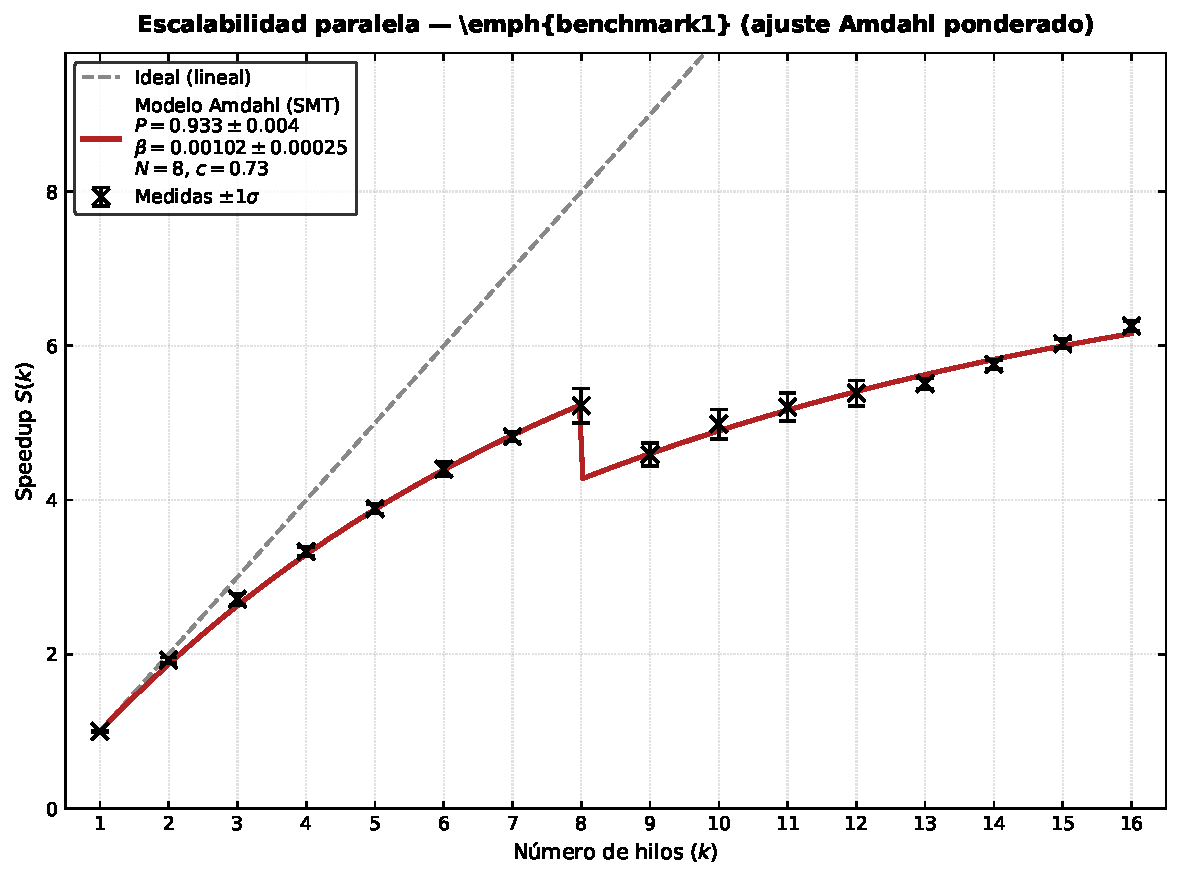
\includegraphics[width=1\textwidth]{Fig14.pdf}
    \caption{Escalabilidad paralela del motor multihilo sobre \emph{benchmark1}: \emph{speedup} empírico $S(k) = T_1/T_k$ (marcadores $\pm 1\sigma$) frente al ideal lineal y al ajuste del modelo de Amdahl con tramo SMT ($P$, $\beta$, $N=8$ núcleos físicos, $c=0{,}73$).}
    \label{fig:paralelismo_speedup}
\end{figure}

La eficiencia de la paralelización se evalúa mediante el \emph{speedup} empírico $S(k) = T_1 / T_k$, donde $T_1$ es el tiempo con un solo hilo y $T_k$ el tiempo con $k$ hilos concurrentes.
En la máquina de referencia ($8$ núcleos físicos, $16$ hilos lógicos), se obtiene $T_1 \approx 1\,121$\,ms y un \emph{speedup} máximo medido de $S(16) \approx 6{,}3$, frente a un ideal de $16$.
La curva no es lineal: hasta $k = 8$ el escalado es claramente sublineal pero monótono ($S(8) \approx 5{,}2$), coherente con una fracción serial residual pequeña pero no nula.
Al cruzar el umbral de núcleos físicos ($k = 9$), el tiempo medio empeora transitoriamente ($T_9 > T_8$), fenómeno atribuible a la contención por \emph{Simultaneous Multithreading}  (SMT) \cite{tullsen1995simultaneous} cuando todos los núcleos físicos ya están saturados; a partir de $k \approx 12$ el \emph{speedup} supera de nuevo ese mínimo y continúa creciendo con pendiente mucho más suave hasta $k = 16$.

Al haber erradicado exclusiones mutuas (\texttt{std::mutex}) y bloqueos de sincronización en el \emph{hot path} del motor ---cada lote de escenarios se lanza con \texttt{std::async} sobre buffers locales---, la limitación observada no proviene de contención software sino del techo de Amdahl y del reparto de recursos hardware al superar $N$ hilos físicos.

Haciendo un ajuste ponderado por la incertidumbre de cada punto ($\pm 1\sigma$) a la función (\ref{eq:amdahl_best}) obtenemos $P = 0{,}933 \pm 0{,}004$ y $\beta = (1{,}0 \pm 0{,}3)\times 10^{-3}$, es decir, más del $93\,\%$ del tiempo de cómputo escala con el paralelismo por lotes y el overhead de gestión de hilos es marginal en el rango medido.

El parámetro $c = 0{,}73$ no se estima en este benchmark, sino que se fija a partir de una micro-prueba de arquitectura: sobre un único núcleo físico se somete a la FPU a carga sostenida (operaciones de coma flotante vectoriales) y se compara el rendimiento con un hilo lógico activo frente a dos hilos lógicos simultáneos en el mismo núcleo; la ratio de mejora observada ($\approx 73\,\%$ de un núcleo físico adicional, no $100\,\%$) se incorpora como constante \texttt{HT\_EFFICIENCY} en el script de ajuste.
Ese experimento auxiliar no forma parte del binario \texttt{integration\_tests.exe}, pero justifica por qué el modelo atenúa el aporte de cada hilo más allá de $N$ en lugar de extrapolar el escalado lineal de los núcleos físicos.
En conjunto, la Figura~\ref{fig:paralelismo_speedup} muestra un motor sustancialmente paralelizable en la cartera de referencia, con buena eficiencia hasta saturar los núcleos físicos y ganancias marginales ---pero positivas--- en el tramo SMT, sin pretender acercarse al ideal lineal global ($S(k) = k$) que la ley de Amdahl proscribe cuando persiste una fracción serial $(1-P) \approx 7\,\%$.

%COMENTAR ESCALADO CON ACTIVOS??

\subsection{Discusión global y conclusiones del análisis}

El capítulo de resultados cierra el ciclo abierto en la introducción: la brecha entre el prototipado cuantitativo en lenguajes de alto nivel y un motor apto para producción exige articular la valoración de instrumentos, la eficiencia del muestreo y la eficiencia de ejecución en CPU.
La discusión global resume cómo los hallazgos de cada bloque se complementan en ese sentido.

En el plano de la \textbf{eficiencia algorítmica estructural}, la Figura~\ref{fig:convergencia_var_es} muestra que el generador aleatorio condiciona la precisión alcanzable a igual presupuesto de simulaciones.
Sobol, con puente browniano, estrecha las bandas de error y acelera el decaimiento del error relativo por debajo de la referencia $\mathcal{O}(N^{-1/2})$; en la práctica, equivale a reducir el error entre tres y cinco veces a igual $N$, o a alcanzar con $2^{15}$ escenarios una precisión que Mersenne Twister solo obtiene cerca de $2^{17}$.
Las tres configuraciones convergen, además, hacia magnitudes de VaR y ES del orden de $13\,350$--$13\,370$ sobre \texttt{benchmark1}, sin sesgo sistemático apreciable entre generadores; cifras creíbles para una cartera con valor inicial del orden de $18\,800$ y exposición predominante a renta variable y derivados.
Las variables antitéticas ofrecen una lectura más matizada ---no mejoran de forma consistente respecto a MT en este escenario---, lo que subraya que una reducción de varianza válida en dimensión baja no se transfiere automáticamente a colas heterogéneas multi-activo.

En el plano de la \textbf{eficiencia algorítmica computacional}, los benchmarks de HPC abordan el coste que permanece una vez fijado $N$.
El contraste RowMajor/ColMajor (Figura~\ref{fig:benchmark_layout_speedup_activos}) cuantifica el impacto de alinear el almacenamiento de $Z \in \mathbb{R}^{F \times S}$ con el patrón fila a fila de \texttt{simulatePathPnL}; a $2\,048$ activos, la ventaja relativa alcanza el $36\,\%$, y el profiling con VTune (Figuras~\ref{fig:vtune_layout} y~\ref{fig:vtune_layout_escala}) atribuye la brecha a una mayor fracción de tiempo aritmético frente a tráfico de memoria en RowMajor.
Paralelamente, el escalado multihilo (Figura~\ref{fig:paralelismo_speedup}) muestra que la orquestación por lotes sin estado compartido alcanza $P \approx 0{,}93$ y un \emph{speedup} de $6{,}3\times$ en la máquina de referencia, con la degradación esperable en el tramo SMT.
Localidad de datos y paralelismo entre escenarios atacan cuellos de botella distintos ---coste por trayectoria cuando $F$ crece frente a reparto de trayectorias cuando $N$ crece---.

\paragraph{Cumplimiento de criterios de aceptación.}
La campaña experimental confirma el cumplimiento de los umbrales \texttt{CA-01}--\texttt{CA-07} fijados en la Tabla~\ref{tab:criterios_aceptacion}: banda de $\text{VaR}_{99\%}$ con Sobol un $40\,\%$ más estrecha que con MT a $N=2\,048$ (\texttt{CA-01}); error relativo del $\text{ES}_{97{,}5\%}$ de $0{,}008\,\%$ con Sobol frente a $0{,}039\,\%$ con MT a $N=2^{17}$ (\texttt{CA-02}); exponente $\alpha \approx -0{,}69$ en el $\text{ES}_{97{,}5\%}$ con Sobol (\texttt{CA-03}); $S(8)\approx 5{,}2$ (\texttt{CA-04}); $P=0{,}933\pm 0{,}004$ (\texttt{CA-05}); ratio ColMajor/RowMajor de $1{,}36$ a $2\,048$ activos (\texttt{CA-06}); y convergencia hacia el mismo orden de magnitud ($13\,350$--$13\,370$) entre generadores (\texttt{CA-07}).

Leídos en conjunto, los resultados validan el objetivo general del proyecto en sus tres frentes entrelazados.
La modelización multi-activo con correlación y Hull--White produce estimaciones de cola estables y reproducibles; el diseño algorítmico del muestreo (Sobol, puentes brownianos, esquemas de error) mejora la eficiencia estadística sin sustituir el tasador; y las optimizaciones de ejecución (Eigen/BLAS, \texttt{matrixLayout}, \texttt{std::async}, profiling) hacen viable en CPU lo que, en un entorno interpretado, resultaría prohibitivo para los volúmenes de cómputo que describe la motivación del trabajo.
En un despliegue real, el tiempo total combina las tres palancas: el modelo define \emph{qué} calcular; la reducción de varianza reduce cuántos escenarios hacen falta; y la ingeniería de bajo nivel comprime el coste de cada uno.

% --- BLOQUE 3: GESTIÓN DEL PROYECTO (Económico y Temporal) ---

\section{Planificación y metodología de trabajo}

A continuación, se detallan la metodología adoptada, el desglose de tareas, la asignación de recursos y el análisis de riesgos asociados.

\subsection{Metodología de trabajo y adaptaciones}

Para el desarrollo de este proyecto se ha optado por una metodología iterativa e incremental, adaptada a los entornos de investigación y desarrollo científico-financiero. A diferencia de las metodologías tradicionales en cascada (Waterfall), el enfoque iterativo permite validar los desarrollos matemáticos y el rendimiento del código de manera continua, minimizando el riesgo de arrastrar errores de concepto o cuellos de botella en la ejecución.

La pertinencia de esta metodología en el ámbito del \textit{Fintech} está justificada por la necesidad de converger de forma eficiente entre la teoría financiera y la eficiencia computacional. El ciclo de vida de cada funcionalidad implementada (como las variables antitéticas, las secuencias de Sobol o los puentes brownianos) ha seguido un esquema de cuatro pasos:
\begin{enumerate}
    \item \textbf{Modelización matemática:} Comprensión teórica y diseño algorítmico del componente.
    \item \textbf{Prototipado rápido:} Validación de la convergencia y resultados en entornos de alto nivel.
    \item \textbf{Implementación en C++:} Codificación modular integrada mediante CMake, aplicando buenas prácticas de programación orientada a objetos y gestión de memoria.
    \item \textbf{Optimización y Perfilado:} Refactorización del código para maximizar el rendimiento computacional.
\end{enumerate}

\subsubsection*{Adaptación metodológica: Integración de IA Generativa}
De nuevo, se muestra al final del documento cómo se ha integrado el uso de IA generativa en el desarrollo de este trabajo.

\subsection{Desglose de tareas y justificación de recursos}

El proyecto se ha dimensionado para una dedicación total de 180 horas (6 ECTS), distribuidas de forma realista a lo largo de las distintas fases del ciclo de vida del software y la investigación. 

\subsubsection{Estructura de Desglose de Trabajo (WBS/EDT)}
A continuación, se detallan las tareas específicas que componen el proyecto, justificando la carga horaria asignada a cada una de ellas:

\begin{table}[h]
\centering
\small
\begin{tabular}{|l|p{11cm}|c|}
\hline
\textbf{Fase/Código} & \textbf{Descripción de la Actividad} & \textbf{Horas} \\ \hline
\textbf{Fase 1} & \textbf{Investigación Inicial, Fundamentos y Prototipado} & \textbf{30 h} \\ \hline
T1.1 & Búsqueda bibliográfica y revisión del estado del arte en la estimación de VaR/ES. Formulación teórica inicial de las matemáticas del motor, contemplando variables antitéticas, secuencias de Sobol y puentes brownianos. & 13 h \\ \hline
T1.2 & Reunión inicial de alineación con el tutor del TFM para delimitar el alcance técnico, matemático y computacional del proyecto, validando el cronograma propuesto. & 5 h \\ \hline
T1.3 & Desarrollo de un script preliminar en Python para simular trayectorias financieras y generar un dataset sintético de referencia. Este prototipo permite obtener resultados de control para la posterior validación estadística del motor. & 12 h \\ \hline
\textbf{Fase 2} & \textbf{Diseño de Arquitectura Base y Configuración del Entorno} & \textbf{36 h} \\ \hline
T2.1 & Diseño estructural e implementación incremental de las clases core en C++ (generadores de sendas, objetos de mercado y cálculo estadístico). Estructuración de la lógica base para el procesamiento secuencial de las simulaciones. & 24 h \\ \hline
T2.2 & Migración del proyecto hacia un entorno de construcción modular y escalable mediante CMake. Gestión de dependencias e inclusión de Boost para tests unitarios y la biblioteca de álgebra lineal Eigen, sentando las bases para una gestión de memoria óptima. & 12 h \\ \hline
\textbf{Fase 3} & \textbf{Extensión de Activos y Simulación Avanzada} & \textbf{42 h} \\ \hline
T3.1 & Incorporación y modelado de derivados complejos mediante la valoración de opciones europeas y opciones barrera. Implementación de técnicas avanzadas de reducción de varianza empleando secuencias de Sobol y puentes brownianos en C++. & 24 h \\ \hline
T3.2 & Formulación matemática e integración de la dinámica de tipos de interés mediante el modelo de Hull-White. Extensión de las capacidades del simulador para permitir el modelado de curvas y la valoración de bonos de la cartera. & 18 h \\ \hline
\textbf{Fase 4} & \textbf{Calibración, Perfilado y Optimización de Rendimiento} & \textbf{36 h} \\ \hline
T4.1 & Estudio experimental del entorno físico de ejecución mediante la medición y análisis de la eficiencia de los cores de la CPU, evaluando el impacto del hardware en los tiempos de cómputo. & 10 h \\ \hline
T4.2 & Pruebas de rendimiento iterativas y perfilado de código (\textit{profiling}) enfocado en mitigar fallos de caché (\textit{cache missing}) aprovechando el alineamiento de Eigen. Desarrollo y aplicación de una generalización de la ley de Amdahl para medir el porcentaje paralelizable real del código. & 26 h \\ \hline
\textbf{Fase 5} & \textbf{Documentación, Redacción de la Memoria y Cierre} & \textbf{36 h} \\ \hline
T5.1 & Redacción iterativa y continua de la memoria técnica del TFM (introducción, marco matemático, arquitectura en C++, optimizaciones y resultados), en paralelo con el avance del desarrollo. & 30 h \\ \hline
T5.2 & Tutorías periódicas de seguimiento con el tutor para la revisión del documento técnico y preparación del material de apoyo audiovisual para la defensa pública ante el tribunal. & 6 h \\ \hline
\multicolumn{2}{|r|}{\textbf{TOTAL HORAS DEL PROYECTO}} & \textbf{180 h} \\ \hline
\end{tabular}
\caption{Desglose detallado de tareas (WBS) y distribución final de horas del TFM.}
\label{tab:wbs}
\end{table}
\clearpage

\subsection{Cronograma seguido en el proyecto}

La secuenciación de las fases descritas se ha estructurado de manera lógica para garantizar que ninguna fase de desarrollo comenzara sin los fundamentos teóricos previos necesarios, cumpliendo estrictamente con el hito final de entrega de la memoria.

\begin{figure}[h!]
    \centering
    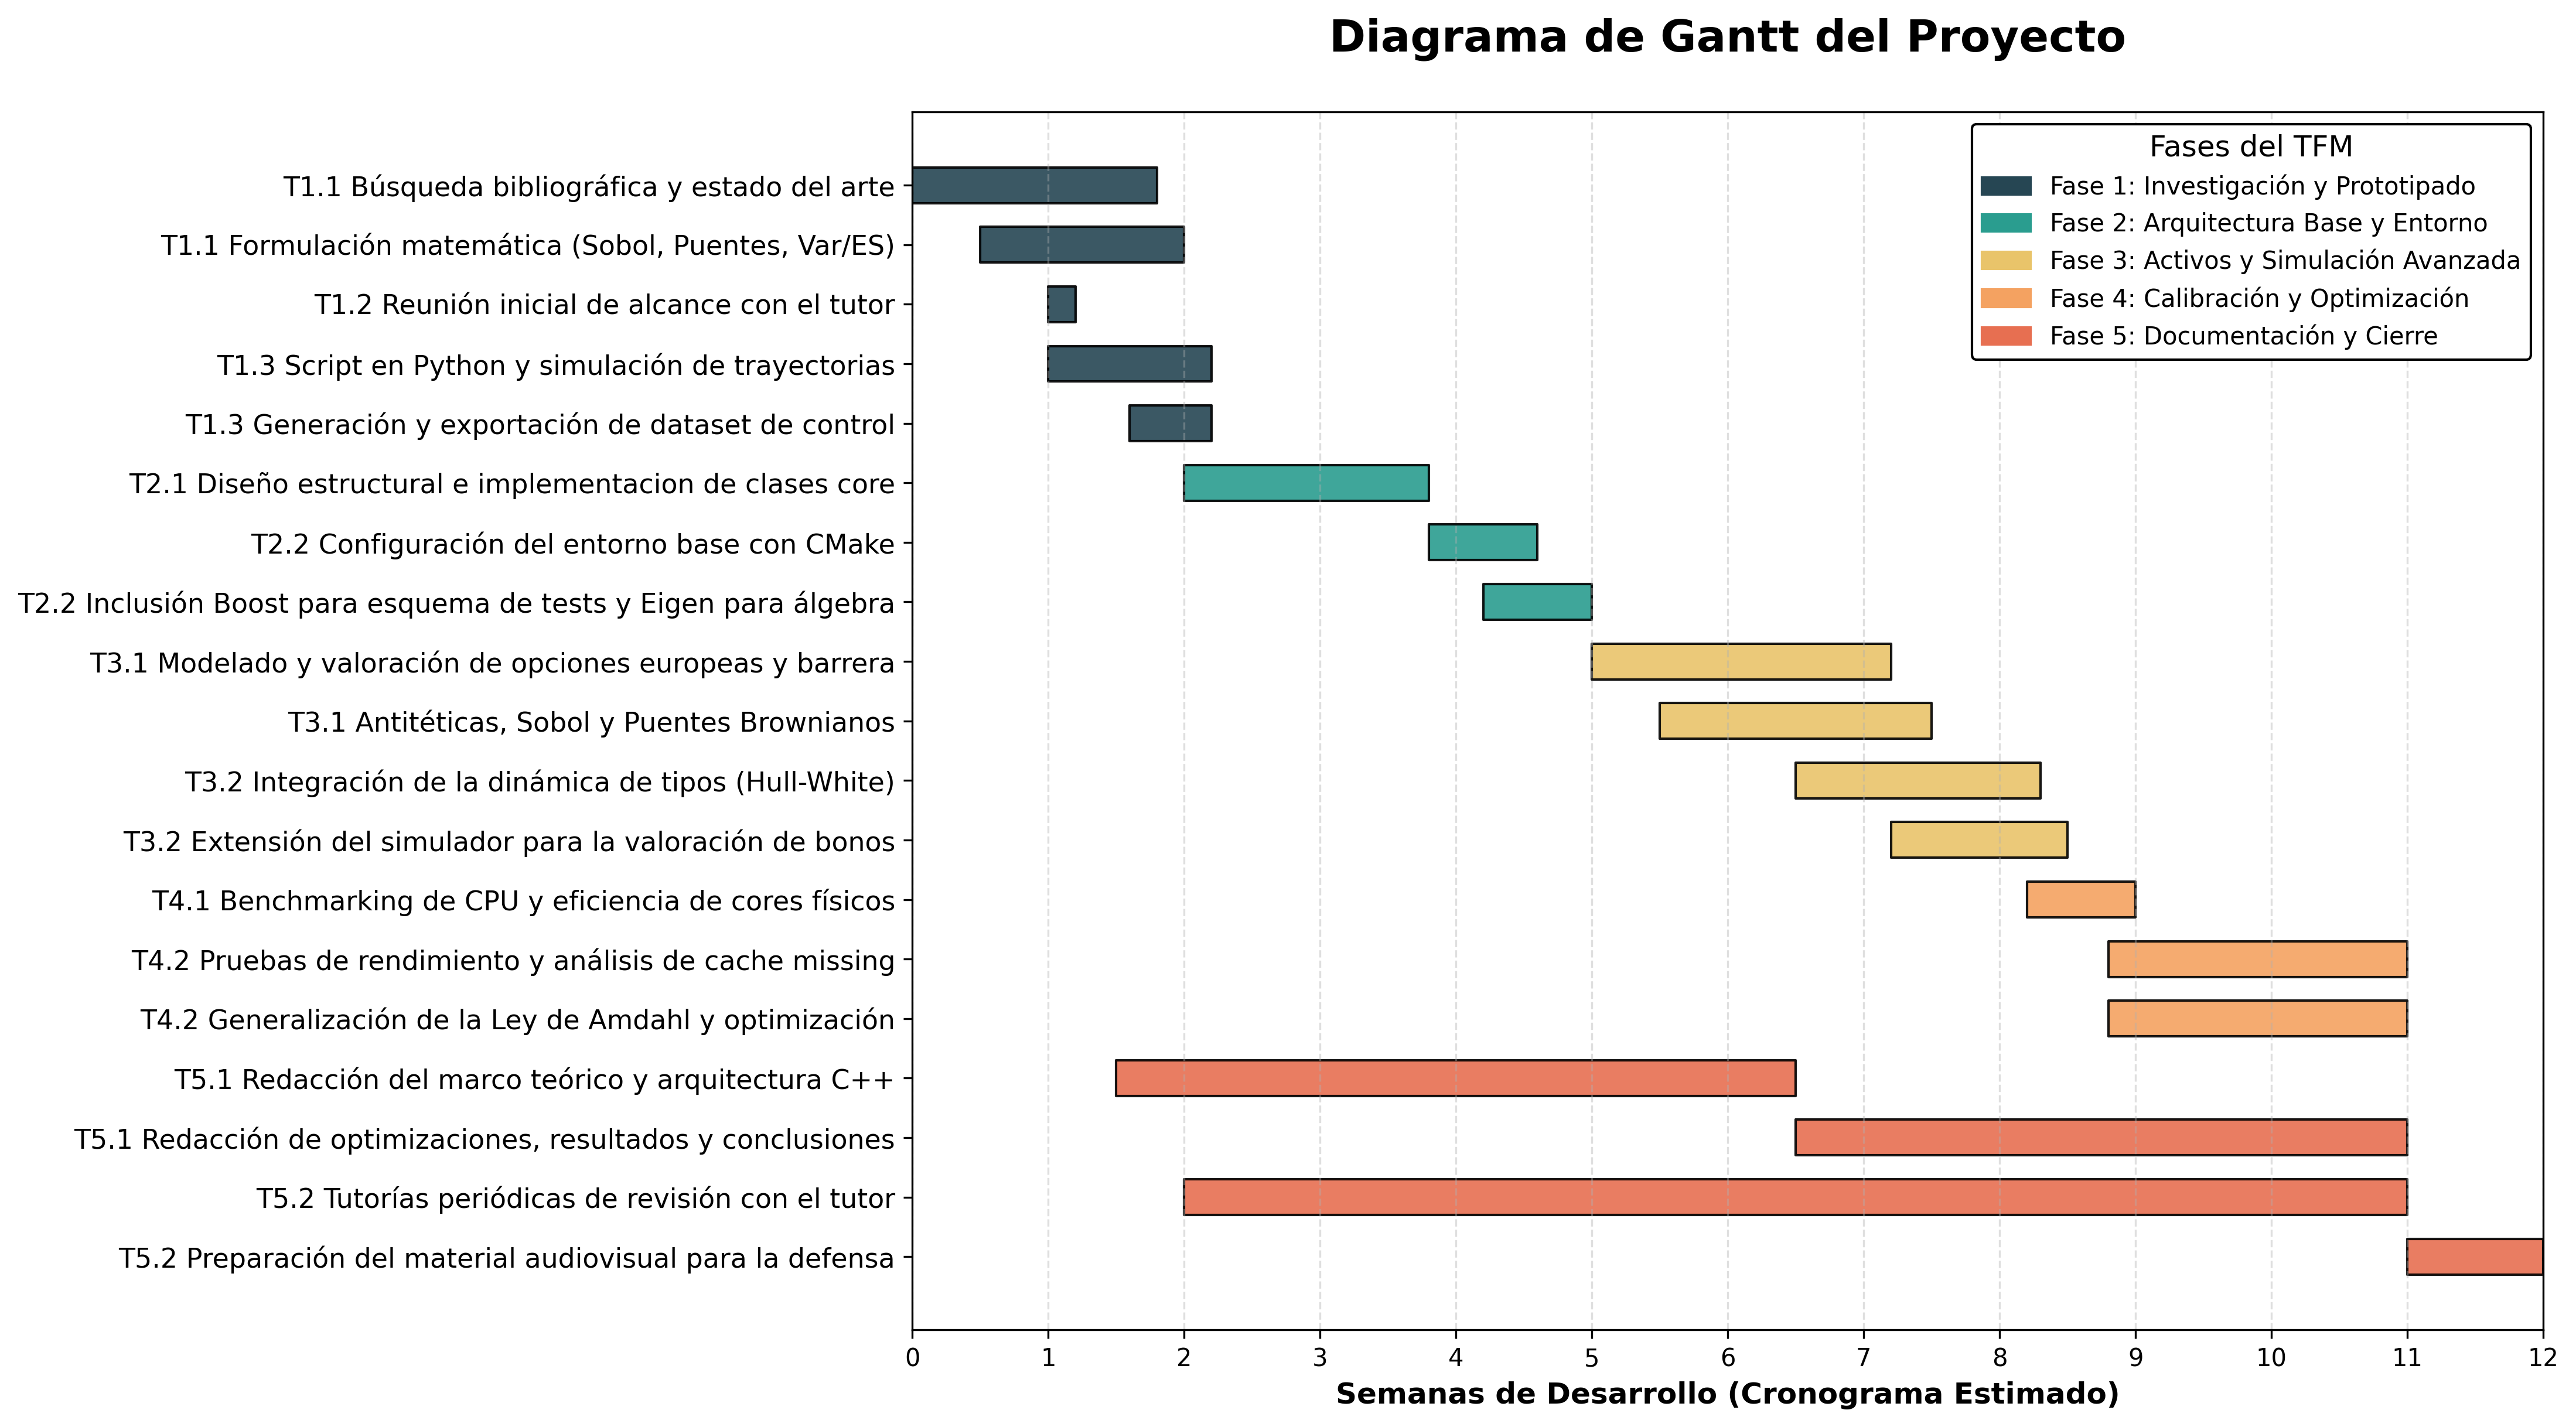
\includegraphics[width=\textwidth]{Fig15.png}
    \caption{Diagrama de Gantt del proyecto.}
    \label{fig:gantt}
\end{figure}

\subsection{Plan de gestión de riesgos}

Dada la complejidad técnica y el límite estricto de tiempo (180 horas), se ha elaborado un plan de riesgos proactivo para identificar potenciales desviaciones y establecer planes de contingencia adecuados.

% Fragmento LaTeX: matriz de riesgos del TFM
% Requiere en el preámbulo: \usepackage{caption}

\vspace{1em}
\noindent
\begin{minipage}{\linewidth}
\centering
\small
\begin{tabular}{|p{4.5cm}|c|c|p{7.9cm}|}
\hline
\textbf{Riesgo identificado} & \textbf{Prob.} & \textbf{Impacto} & \textbf{Estrategia de mitigación / contingencia} \\ \hline

\textbf{R1. Sesgo o falta de convergencia estadística}
(p.\,ej.\ implementación incorrecta de Sobol, puente browniano o emparejamiento antitético; estimación inadecuada de VaR/ES con muestras finitas). &
Media & Alto &
\textbf{Mitigación:} Validar primero los generadores en experimentos de baja dimensión (estimación de $\pi$, convergencia de cuantiles) antes de integrarlos en el motor.
Comparar sistemáticamente Mersenne Twister, antitéticas y Sobol sobre la misma cartera (\texttt{convergencia\_cartera\_base}).
Tests unitarios de \texttt{MonteCarloErrorPolicy} para cada esquema de error (bootstrap, pares antitéticos, lotes Sobol). \\ \hline

\textbf{R2. Cuello de botella de rendimiento no dominado por el paralelismo}
(revaloración secuencial por activo $\times$ escenario; fracción serial elevada; penalización por \emph{layout} de memoria o contención en hilos). &
Media & Media &
\textbf{Mitigación:} Arquitectura modular con \emph{hot path} acotado (\texttt{simulateFinalValue}); paralelismo por lotes independientes (\texttt{std::async}) con RNG por hilo.
Reservar fase explícita de \textit{benchmarking} y \textit{profiling} (Amdahl, escalado por número de activos, RowMajor vs.\ ColMajor).
Contingencia: reducir $N$ o tamaño de cartera en pruebas de estrés sin invalidar las conclusiones cualitativas del escalado. \\ \hline

\textbf{R3. Errores en la agregación multi-activo o en el acoplamiento con tipos}
(matriz de correlación no definida positiva, dimensiones inconsistentes entre cartera y factor de tasa Hull--White, descuento incorrecto). &
Baja & Alto &
\textbf{Mitigación:} Descomposición de Cholesky con validación previa (\texttt{Eigen::LLT}); tests de integración sobre carteras de referencia con valor inicial y P\&L conocidos.
Revisión de la dimensionalidad de shocks: $\text{numFactores} = \text{numActivos} + \mathbb{1}_{\{\text{rateModel}\}}$. \\ \hline

\textbf{R4. Retrasos por entorno de compilación o dependencias externas}
(rutas locales de Boost/Eigen en CMake; incompatibilidades entre plataformas o versiones de librerías). &
Baja & Media &
\textbf{Mitigación:} Diseño modular por bibliotecas (\texttt{Asset}, \texttt{Random}, \texttt{MontecarloEngine}, etc.) con interfaces acotadas.
Documentar dependencias mínimas (Boost.Random/Sobol, Boost.Test, Eigen header-only) y fijar versiones probadas.
Contingencia: concentrar la demostración en el entorno de desarrollo validado y automatizar la ejecución de \texttt{light\_tests} e \texttt{integration\_tests} tras cada cambio estructural. \\ \hline

\textbf{R5. Desviación temporal por ampliación del alcance funcional}
(incorporar activos exóticos adicionales, métricas de sensibilidad o técnicas no previstas como MLMC/GPU). &
Alta & Baja &
\textbf{Mitigación:} Delimitar el alcance a VaR/ES sobre P\&L de cartera con los cuatro tipos de activo ya soportados; tratar ML, cuántica y aceleradores heterogéneos solo en el estado del arte.
Priorizar en la planificación las palancas adoptadas (QMC + CPU) frente a extensiones accesorias. \\ \hline

\end{tabular}
\captionof{table}{Matriz de riesgos y planes de mitigación del desarrollo del motor Monte Carlo.
Escala cualitativa: probabilidad \textit{Alta / Media / Baja}; impacto \textit{Alto / Media / Baja}.}
\label{tab:riesgos}
\end{minipage}
\vspace{1em}
 % Separación con la siguiente sección o texto

\section{Presupuesto}
\label{sec:presupuesto}

En este apartado se detalla el análisis económico de los recursos necesarios para el diseño, desarrollo e implementación de este Trabajo de Fin de Máster. El presupuesto se ha estructurado en cuatro partidas principales: recursos humanos, activos de hardware, licencias de software y costes indirectos.

\subsection{Recursos Humanos}

Esta partida representa el coste más significativo del proyecto, ya que contempla el tiempo de dedicación del personal especializado. Los valores salariales han sido extraídos de la \textit{Manfred Salary Guide 2026} \cite{manfred2026}, seleccionando los perfiles que mejor se ajustan a la naturaleza técnica y de gestión de este trabajo.

Para el cálculo del coste horario, se ha tomado como referencia un estándar de 1.800 horas laborales anuales (jornada completa estándar en España). El desglose detallado se presenta en la Tabla \ref{tab:rrhh}:

\begin{itemize}
 \item \textbf{Quantitative Developer (QDev) (Junior):} Se ha asignado un salario base bruto de aproximadamente 33.850 \euro{} anuales. Al incorporar un 33\% en concepto de costes de Seguridad Social a cargo de la empresa, el coste total anual asciende a 45.020 \euro{}. Considerando una jornada estándar de 1.800 horas anuales, el coste por hora resultante es de 25,00 \euro/h.
 \item \textbf{Engineering Manager (Senior):} Para las tareas de tutorización y supervisión técnica, se referencia un salario bruto de 75.000 \euro{} anuales (ajustado a la baja respecto a la fuente de referencia \cite{manfred2026}). Tras sumar el 33\% de costes empresariales, el coste anual total es de 99.750 \euro{}, lo que implica un coste de 55,42 \euro/h.
\end{itemize}

\begin{table}[h!]
\centering
\small
\begin{tabularx}{\textwidth}{lXXX}
\toprule
\textbf{Rol (Ref. Manfred 2026)} & \textbf{Coste/Hora (est.)} & \textbf{Horas} & \textbf{Subtotal} \\ \midrule
Quantitative Developer (QDev)    & 25,00 \euro/h              & 180            & 4.500,00 \euro    \\
Engineering Manager              & 55,42 \euro/h              & 30             & 1.662,60 \euro    \\ \midrule
\textbf{Total RRHH}              &                            &                & \textbf{6.162,60 \euro} \\ \bottomrule
\end{tabularx}
\caption{Desglose de costes de personal incluyendo costes empresariales (Seguridad Social) y adaptado a la carga lectiva del TFM (6 ECTS).}
\label{tab:rrhh}
\end{table}

\subsection{Recursos de Hardware y Equipamiento}

Esta partida comprende el equipamiento físico personal empleado en el desarrollo del algoritmo y en la fase de análisis de rendimiento y gestión de memoria, valorado mediante amortización lineal sobre la duración imputable del proyecto (3 meses).

\begin{table}[h!]
\centering
\small
\begin{tabularx}{\textwidth}{lXXX}
\toprule
\textbf{Dispositivo / Especificación} & \textbf{Valor / Ref.} & \textbf{Uso Imputable} & \textbf{Subtotal} \\ \midrule
Portátil Lenovo (Personal) & 800,00 \euro & 3 meses (Amort.) & 40,00 \euro \\
Monitor (Personal) & 200,00 \euro & 3 meses (Amort.) & 10,00 \euro \\ \midrule
\textbf{Total Hardware} & & & \textbf{50,00 \euro} \\ \bottomrule
\end{tabularx}
\caption{Valoración de equipos y computación.}
\label{tab:presupuesto_hardware}
\end{table}

\subsection{Licencias de Software}

En este apartado se detallan las herramientas y servicios bajo modelo \textit{Software as a Service} (SaaS) necesarios para la redacción y apoyo en el desarrollo. Las licencias de sistemas operativos base se consideran integradas en los costes indirectos para evitar duplicidades contables.

\begin{table}[h!]
\centering
\small
\begin{tabularx}{\textwidth}{lXXX}
\toprule
\textbf{Licencia / Servicio} & \textbf{Coste Mensual} & \textbf{Duración} & \textbf{Subtotal} \\ \midrule
Overleaf Student Plan \cite{overleaf_pricing} & 9,00 \euro & 3 meses & 27,00 \euro \\
Google AI Pro \cite{google_ai_pricing} & 18,17 \euro & 3 meses & 54,51 \euro \\ \midrule
\textbf{Total Software} & & & \textbf{81,51 \euro} \\ \bottomrule
\end{tabularx}
\caption{Desglose de costes de software y servicios SaaS.}
\label{tab:software}
\end{table}

\subsection{Costes Indirectos y Suministros}

Los costes indirectos representan los gastos estructurales necesarios para la ejecución del proyecto: suministro eléctrico, conectividad, licencias de sistemas operativos base y uso de espacios. 

Para la determinación de esta partida, se ha adoptado un criterio de imputación por tipo fijo del 15\% sobre los costes directos totales. Esta cifra se fundamenta en un análisis comparativo entre el marco del Real Decreto 1098/2001 \cite{boe_rd1098_2001} y el Manual de I+D+i del CDTI \cite{cdti_manual_2025}, garantizando una cobertura realista de los gastos generales operativos.

\begin{table}[h!]
\centering
\small
\begin{tabularx}{\textwidth}{lXX}
\toprule
\textbf{Concepto} & \textbf{Base de Cálculo} & \textbf{Subtotal} \\ \midrule
Suma de Costes Directos (CD) & $6.162,60 + 50,00 + 81,51$ & 6.294,11 \euro \\
Gastos Indirectos (15\% s/ CD) & Coeficiente s/ \cite{boe_rd1098_2001, cdti_manual_2025} & 944,12 \euro \\ \midrule
\textbf{Total Indirectos} & & \textbf{944,12 \euro} \\ \bottomrule
\end{tabularx}
\caption{Cálculo de costes indirectos mediante coeficiente porcentual (actualizado).}
\label{tab:indirectos}
\end{table}

\subsection{Resumen del Presupuesto Total}

La Tabla \ref{tab:total} presenta el resumen consolidado. Se incluye el Impuesto sobre el Valor Añadido (IVA) vigente del 21\% sobre la base imponible total.

\begin{table}[h!]
\centering
\small
\begin{tabularx}{0.7\textwidth}{lX}
\toprule
\textbf{Partida} & \textbf{Importe} \\ \midrule
Recursos Humanos & 6.162,60 \euro \\
Hardware & 50,00 \euro \\
Licencias Software & 81,51 \euro \\
Costes Indirectos (15\%) & 944,12 \euro \\ \midrule
\textbf{Base Imponible (Neto)} & \textbf{7.238,23 \euro} \\
IVA (21\%) & 1.520,03 \euro \\ \midrule
\textbf{TOTAL PRESUPUESTO} & \textbf{8.758,26 \euro} \\ \bottomrule
\end{tabularx}
\caption{Resumen consolidado del presupuesto total.}
\label{tab:total}
\end{table}
% --- BLOQUE 4: CIERRE ACADÉMICO ---

\section{Competencias y Relación Académica}

El desarrollo de este Trabajo de Fin de Máster constituye un ejercicio de convergencia de los conocimientos teóricos y prácticos adquiridos a lo largo del programa académico. El proyecto no se plantea como un elemento aislado, sino como la materialización interdisciplinar de las competencias clave del sector \textit{Fintech}: la ingeniería de software de alto rendimiento y los métodos cuantitativos aplicados a las finanzas.

\subsection{Vinculación con las materias del Máster}

El diseño e implementación del motor de simulación de Monte Carlo para el cálculo de VaR (\textit{Value at Risk}) y ES (\textit{Expected Shortfall}) se articula de manera directa en torno a cuatro asignaturas troncales del plan de estudios:

\begin{enumerate}
    \item \textbf{Programación de Altas Prestaciones:} 
    Esta asignatura ha proporcionado el sustrato técnico y metodológico indispensable para la viabilidad del proyecto. La simulación de Monte Carlo es intensiva en cómputo, por lo que la aplicación de los estándares modernos de C++ (C++20), la gestión eficiente de la memoria a través de punteros inteligentes, el paso por referencia y la semántica de movimiento han sido críticos para minimizar la latencia. Asimismo, la automatización del proyecto mediante \texttt{CMake} y el uso de herramientas de perfilado e instrumentación de código para la detección de cuellos de botella provienen directamente de las competencias adquiridas en esta materia.
    
    \item \textbf{Algoritmos de Front Office:} 
    En esta asignatura adquirí los conocimientos teóricos y prácticos sobre cómo el entorno de \textit{trading} y la estructuración de productos exigen algoritmos de valoración en tiempo real donde la velocidad de convergencia es crítica. Gracias a las técnicas de simulación cuantitativa estudiadas durante el curso, supe cómo abordar el desarrollo del motor implementando las secuencias de baja discrepancia de Sobol y los puentes brownianos. Aplicar estos conceptos avanzados me permitió acelerar la convergencia matemática del simulador, logrando que el cálculo de VaR y ES requiera un menor número de iteraciones. De este modo, traduje el enfoque práctico de la materia en optimizaciones medibles sobre \texttt{benchmark1}, relevantes para escenarios de recálculo intra-día pero sin implementar el pipeline operativo de producción descrito en las limitaciones del §1.3.

    
    \item \textbf{Algoritmos de Back Office:} 
    Esta materia me aportó una visión profunda e indispensable sobre la gestión global de riesgos, el \textit{stress testing} y las exigencias de cumplimiento normativo bajo los marcos de Basilea III y IV. Lo aprendido en clase sobre la agregación de carteras y el control de riesgos me sirvió como guía para estructurar la salida estadística de mi motor con la rigurosidad que exige el sector. En lugar de limitarme a un cálculo matemático aislado, apliqué los criterios regulatorios estudiados para sistematizar la medición del VaR y el \textit{Expected Shortfall}, asegurándome de que la arquitectura modular diseñada sea capaz de soportar con solidez los procesos de fin de día (\textit{end-of-day processing}) que se ejecutan en una entidad financiera real.
    
    \item \textbf{Introducción a los Mercados Financieros:} 
    Esta materia aportó el contexto conceptual y el entendimiento del entorno económico sobre el cual opera el software. Para poder modelizar los factores de riesgo y simular las trayectorias de los activos, es imprescindible comprender la naturaleza de las variables financieras (volatilidad, rendimientos, tipos de interés) y el comportamiento de los diferentes productos subyacentes. La interpretación de los resultados del VaR y el ES carecería de sentido analítico sin la base teórica de esta asignatura sobre cómo se comportan los mercados y cómo impacta el riesgo de mercado en los balances financieros.
\end{enumerate}

\subsection{Desglose de competencias generales}

Más allá del conocimiento específico de las asignaturas, la ejecución autónoma de este TFM ha permitido consolidar y demostrar un conjunto de competencias generales transversales de nivel de máster:

\begin{itemize}
    \item \textbf{Capacidad de modelización matemática y abstracción:} Habilidad para trasladar desarrollos matemáticos teóricos complejos (reducción de varianza con variables antitéticas, generación estocástica) a código fuente estructurado, modular y ejecutable sin perder la rigurosidad científica.
    \item \textbf{Pensamiento crítico y resolución de problemas de ingeniería:} Capacidad para diagnosticar ineficiencias en el rendimiento computacional, analizar el uso de la caché y los recursos de hardware, y proponer soluciones óptimas de refactorización bajo criterios de ingeniería de software profesional.
    \item \textbf{Autonomía en la investigación científica:} Destreza en la búsqueda, selección y síntesis de literatura financiera e informática indexada, permitiendo estructurar un estado del arte sólido y validar los resultados del motor frente a modelos de control consolidados.
    \item \textbf{Planificación y gestión de proyectos:} Capacidad para estimar, secuenciar y mitigar los riesgos de un proyecto tecnológico complejo con una restricción temporal estricta de 180 horas, coordinando hitos de entrega y revisiones periódicas con la dirección académica.
\end{itemize}

% Fragmento LaTeX: conclusiones y líneas futuras.
% Insertar como capítulo/sección final de la memoria, tras el capítulo de resultados.

\section{Conclusiones y futuras líneas}

\subsection{Conclusiones generales del trabajo}

Este Trabajo de Fin de Máster ha diseñado, implementado y evaluado un motor de simulación Monte Carlo en C++ para la estimación de VaR y ES sobre carteras multi-activo con dependencias entre factores de riesgo y tipos de interés.
La pregunta que abría la motivación del proyecto ---cuánto margen queda en un Monte Carlo transparente antes de tener que abandonarlo--- encuentra aquí su respuesta empírica: no se trataba de probar que C++ es más rápido que un prototipo interpretado, sino de localizar, con medidas, dónde se pierde precisión y dónde se pierde tiempo cuando cada escenario sigue siendo revalorizable.

La aportación más concreta del trabajo se concentra en tres hallazgos que el Capítulo~6 desarrolla y mide sobre la cartera \texttt{benchmark1}:

\begin{enumerate}
    \item \textbf{El cuasi-Monte Carlo comprime el presupuesto de escenarios.}
    Hemos demostrado que Sobol con puente browniano no es un refinamiento accesorio del muestreo pseudoaleatorio: a igual $N$, reduce entre tres y cinco veces el error de VaR y ES.
    Más allá de esa cifra puntual, lo relevante es que la convergencia del error cae más deprisa que la referencia $\mathcal{O}(N^{-1/2})$ del Monte Carlo clásico: la cola deja de fluctuar antes, sin empujar el estimador hacia otro valor ---las tres configuraciones convergen al mismo orden de magnitud---, sino acortando el camino hasta una estimación estable.

    \item \textbf{El paralelismo tiene un techo medible, y SMT forma parte de él.}
    Hemos formulado y validado experimentalmente una generalización de la ley de Amdahl con tramo SMT (ecuación~\ref{eq:amdahl_best}) que captura lo que un ajuste clásico no explica: la curva empírica no es lineal, el ajuste encaja de forma visible y el modelo reproduce fenómenos que, a priori, resultan contraintuitivos ---como que $8$ hilos puedan rendir mejor que $9$ al cruzar el umbral de núcleos físicos--- porque el segundo hilo lógico no equivale a un núcleo adicional.
    El motor escala gracias a lotes de trayectorias independientes, pero tampoco promete un speedup ilimitado: la fracción serial residual y la contención por SMT delimitan dónde termina el margen en CPU.

    \item \textbf{El \emph{layout} de memoria condiciona el coste por trayectoria cuando la cartera crece.}
    Hemos visto que alinear el almacenamiento de la matriz de shocks con el patrón fila a fila de la revaloración no es un detalle de implementación: cuando el número de factores crece, la diferencia entre RowMajor y ColMajor se hace sistemática, y el profiling con VTune confirma que no se trata de ruido experimental sino de un desplazamiento del tiempo de CPU de acceso a memoria hacia aritmética vectorial.
    Es una palanca distinta del paralelismo entre escenarios: no reparte más trayectorias, sino abarata cada una conforme la cartera se hace más pesada.
\end{enumerate}

Los tres apuntan al mismo sitio: el margen estaba en el método, pero hacía falta implementarlo, medirlo y no renunciar a la revaloración explícita para verlo.

Las conclusiones del trabajo pueden sintetizarse, además, en los siguientes puntos:

\begin{itemize}
    \item \textbf{Motor funcional y modular.}
    Se ha construido una arquitectura que separa dominio financiero, generación de aleatorios, simulación y cálculo de métricas, integrando renta variable (GBM), opciones europeas y de barrera, bonos con dinámica Hull--White y correlación entre activos y factor de tipos.
    La validación mediante pruebas unitarias, de integración y experimentos reproducibles sobre la cartera \texttt{benchmark1} confirma que el sistema produce estimaciones de cola coherentes y estables en el alcance definido.

    \item \textbf{Eficiencia estadística del muestreo.}
    La comparación sistemática entre Mersenne Twister, variables antitéticas y Sobol con puente browniano demuestra que el cuasi-Monte Carlo mejora de forma sustancial la convergencia de VaR y ES a igual número de simulaciones, con esquemas de error adaptados a cada generador.
    La elección del muestreador condiciona directamente el presupuesto de escenarios necesario para alcanzar una precisión operativa.

    \item \textbf{Rendimiento computacional en CPU.}
    El motor paraleliza eficazmente el trabajo entre escenarios ($P \approx 0{,}93$, \emph{speedup} de $6{,}3\times$ en la máquina de referencia) y beneficia de decisiones de bajo nivel ---en particular, el almacenamiento RowMajor de la matriz de shocks--- cuando el número de factores de riesgo crece.
    El profiling con VTune corrobora que la optimización de memoria y la vectorización vía Eigen/BLAS no son accesorios, sino componentes del rendimiento global.

    \item \textbf{Solución justificada frente a alternativas.}
    Frente a metamodelos de aprendizaje automático, simulación cuántica o despliegue en GPU/TPU, la propuesta adoptada prioriza la trazabilidad escenario a escenario, la madurez tecnológica y la viabilidad sobre infraestructura CPU ya disponible en la industria financiera, optimizando el Monte Carlo clásico con técnicas consolidadas (QMC, Cholesky, paralelismo nativo) en lugar de sustituir el tasador.

    \item \textbf{Integración de competencias del Máster.}
    El trabajo justifica de forma explícita la utilización de tres disciplinas adquiridas en el programa.
    En primer lugar, la \emph{valoración de activos y modelos de riesgo}: implementación y validación de GBM, opciones, bonos con Hull--White, correlación entre factores y estimación coherente de VaR y ES sobre P\&L simulado.
    En segundo lugar, la \emph{eficiencia algorítmica estructural}: comparación rigurosa de técnicas de reducción de varianza (Mersenne Twister, antitéticas, Sobol con puente browniano) y esquemas de error adaptados a cada generador.
    En tercer lugar, la \emph{eficiencia algorítmica computacional}: paralelismo multihilo, optimización del \emph{layout} de matrices, vectorización vía Eigen/BLAS y caracterización del rendimiento mediante profiling (VTune) y ajuste de la ley de Amdahl.
    La transición desde la formulación financiera hasta un artefacto C++ medido y documentado demuestra que el problema no se resuelve dominando una sola de estas áreas, sino articulándolas de forma coordinada.
\end{itemize}

En conjunto, la evaluación empírica demuestra que el objetivo general del proyecto ---desarrollar un motor Monte Carlo nativo capaz de estimar el riesgo de mercado validando simultáneamente el comportamiento estadístico y temporal del sistema--- se ha cumplido dentro del alcance declarado.
El empuje hacia soluciones opacas no venía del Monte Carlo como método, sino de un Monte Carlo implementado sin medir: esa fue la sospecha que abrió el proyecto, y los tres hallazgos anteriores la confirman.

\subsection{Limitaciones y líneas de trabajo futuro}

El alcance del estudio impone acotaciones que conviene reconocer de forma explícita y que abren direcciones naturales de extensión.

\paragraph{Limitaciones.}
En primer lugar, los parámetros de los modelos (volatilidades, correlaciones, curva de tipos, strikes, barreras) se definen de forma sintética o simplificada, sin una \emph{pipeline} completa de calibración histórica ni de mercado en tiempo real.
En segundo lugar, el universo de instrumentos cubre equity, opciones europeas y de barrera, y bonos con Hull--White de un factor, pero no incluye americanas, derivados de crédito, swaps u otros exóticos; los supuestos de volatilidad y correlación constantes, ausencia de saltos y de fricciones de mercado permanecen vigentes.
En tercer lugar, la paralelización se limita a memoria compartida en CPU: no se ha explorado ejecución distribuida, aceleración en GPU ni despliegue en entornos \emph{cloud}.
Por último, los benchmarks de rendimiento dependen de configuraciones hardware concretas y la escala de cartera se construye replicando \texttt{benchmark1}, lo que controla el experimento pero no agota la heterogeneidad estructural de carteras reales.

\paragraph{Líneas de trabajo futuro.}
A partir de estas limitaciones, las extensiones más prometedoras serían:

\begin{itemize}
    \item \textbf{Ampliación del universo de instrumentos y modelos.} Incorporar opciones americanas, productos de tipos de interés más generales (modelos multifactoriales, LMM) o derivados de crédito, manteniendo la arquitectura modular del motor.

    \item \textbf{Calibración y datos de mercado.} Conectar el motor a fuentes de datos reales y automatizar la calibración de parámetros, acercando el sistema a un flujo operativo de mesa de riesgo.

    \item \textbf{Reducción de varianza avanzada.} Profundizar en técnicas complementarias ---control variates, importance sampling, MLMC--- y reevaluar el papel de las variables antitéticas en carteras con estructuras de cola más heterogéneas, donde los resultados actuales muestran un comportamiento no uniforme.

    \item \textbf{Escalado hardware.} Explorar ejecución distribuida o portabilidad a GPU/TPU para cargas masivas, evaluando el compromiso entre \emph{throughput} y auditabilidad que motivó la elección inicial de CPU.

    \item \textbf{Adaptación dinámica del presupuesto de simulación.} Combinar los esquemas de error ya implementados con criterios de parada basados en la incertidumbre de VaR/ES, de modo que $N$ se ajuste automáticamente a la precisión requerida.

    \item \textbf{Caracterización en mayor escala.} Extender los estudios de \emph{layout} y Amdahl a carteras con estructura de correlación más rica que la replicación por bloques, y a entornos de ejecución controlados (\emph{pinning} de hilos, afinidad NUMA, múltiples procesadores).
\end{itemize}

Ninguna de estas líneas invalida los resultados obtenidos; las sitúan, en cambio, como punto de partida de un motor que ha demostrado viabilidad técnica y que conserva margen de mejora tanto en el plano algorítmico como en el de infraestructura.



\newpage

\printbibliography

\newpage

\section*{Apéndice A: El Teorema del Límite Central y su papel en Monte Carlo}

El método de Monte Carlo está completamente basado en el Teorema del Límite Central (TLC). Este teorema es la razón por la cual podemos fiarnos de la aleatoriedad para obtener respuestas numéricas precisas y es por ello, que voy a dedicar un apéndice a explicarlo de forma muy sencilla, para asegurar que el lector comprende la naturaleza del método. 

Para ver la intuición matemática de forma clara, pensemos en un experimento cotidiano: lanzar dados. Imaginemos una variable aleatoria $X_i$ que representa el resultado de lanzar un único dado de seis caras no trucado, es decir, $X_i \in \{1, 2, \dots, 6\}$. La distribución de probabilidad de esta variable, que llamaremos $\rho(X_i)$, es completamente plana y uniforme: todos los resultados tienen exactamente la misma probabilidad de salir ($1/6$).

Ahora cambiemos las reglas. Supongamos que jugamos con dos dados independientes y definimos una nueva variable, $Y$, que es la suma de ambos: $Y = X_1 + X_2$. Si nos preguntamos si esta nueva variable aleatoria sigue teniendo una distribución equiprobable, la respuesta es un no rotundo. Cualquiera que haya jugado a los dados sabe que es muchísimo más fácil obtener un $7$ que un $12$. Para el $7$ nos sirven combinaciones como 1+6, 2+5 o 3+4, mientras que para el $12$ estamos condicionados a un único escenario: 6+6. Formalmente, la distribución de esta suma ya no es plana, sino triangular, y se calcula matemáticamente como la convolución de $\rho(X_i)$ consigo misma.

¿Qué ocurre si expandimos el juego a $N$ dados? La variable aleatoria que mide la suma total será:
\begin{equation}
    Z_N = \sum_{i=1}^{N} X_i
\end{equation}
Para hallar su distribución exacta, tendríamos que convolucionar $\rho(X_i)$ un total de $N$ veces. Al hacerlo, la distribución de $Z_N$ deja de ser una forma escalonada o geométrica extraña y empieza a dibujar una curva normal (de campana) perfecta, con media $N\mu_X$ y desviación estándar $\sqrt{N}\sigma_X$, donde $\mu_X$ y $\sigma_X$ son la media y la desviación de un solo dado.

\begin{figure}[htbp]
    \centering
    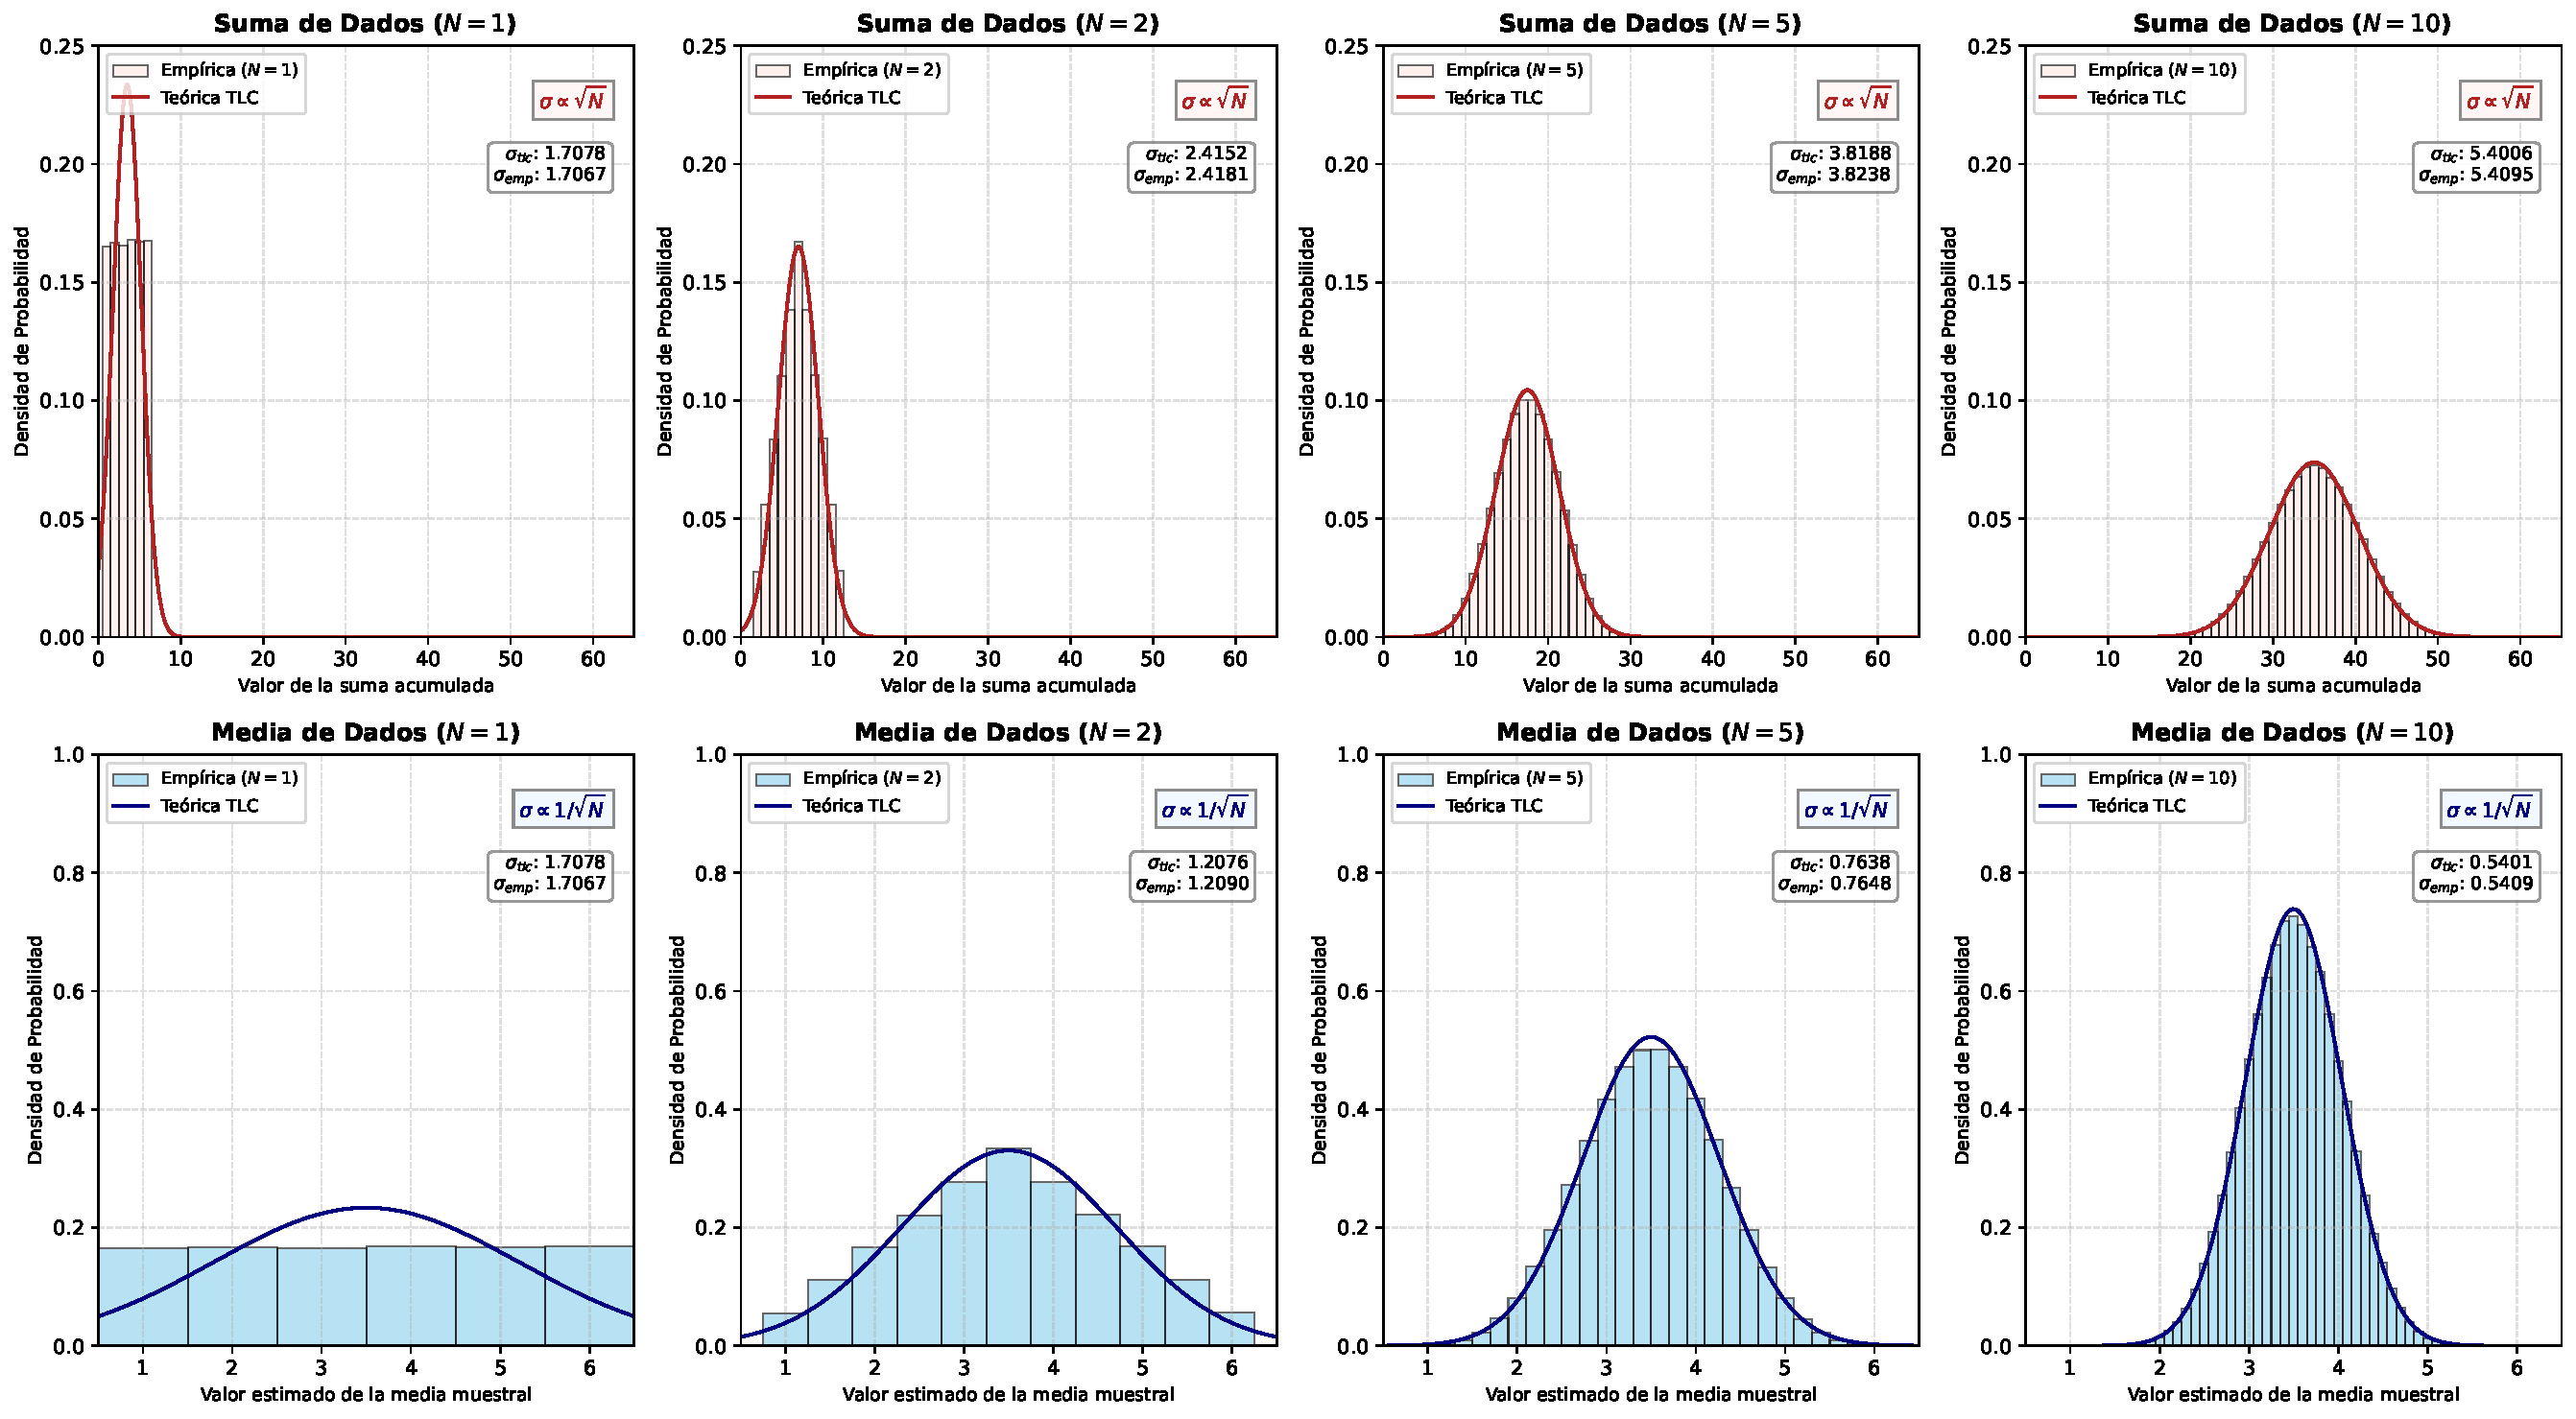
\includegraphics[width=1\textwidth]{Fig16.pdf}
    \caption{Análisis bibliométrico de la evolución temporal de conceptos clave en la literatura financiera cuantitativa (Menciones normalizadas por cada 10,000 artículos).}
    \label{fig:TLC}
\end{figure}

Ahora bien, si en lugar de mirar la suma calculamos el promedio de los $N$ dados, tenemos:
\begin{equation}
    \bar{X}_N = \frac{1}{N} Z_N = \frac{1}{N} \sum_{i=1}^{N} X_i
\end{equation}
Esta variable $\bar{X}_N$ es precisamente el estimador que usamos en nuestras simulaciones de riesgo. Al dividir por $N$, la distribución de la media muestral (la de la media, no la de los dados individuales) es una distribución normal cuya media sigue siendo $\mu_X$, pero su desviación estándar se reduce a:
\begin{equation}
    \sigma_{\bar{X}} = \frac{\sigma_X}{\sqrt{N}}
    \label{eq:error_tlc}
\end{equation}

La ecuación (\ref{eq:error_tlc}) nos está dando precisamente el error en Monte Carlo. Nos dice que la incertidumbre de nuestra estimación decrece a un ritmo de $1/\sqrt{N}$. Por tanto, la precisión no es lineal. Si queremos asegurar con un nivel de confianza estadística que hemos fijado correctamente un decimal en nuestra métrica de riesgo, necesitaremos lanzar $100$ simulaciones ($1/\sqrt{100} = 0.1$). Si nuestro nivel de exigencia sube y queremos asegurar dos decimales de precisión, el esfuerzo computacional no se duplica, sino que se multiplica por cien, obligándonos a lanzar $10,000$ escenarios ($1/\sqrt{10,000} = 0.01$).

La importancia del Teorema del Límite Central es su universalidad. No importa lo caótica, asimétrica o extraña que sea la distribución original de los factores de riesgo de nuestra cartera; al promediar los resultados de los escenarios simulados, la distribución del estimador siempre convergerá hacia una normal. Esto es lo que nos permite hacer estadística, calcular intervalos de confianza rigurosos y acotar con total precisión el error que estamos asumiendon.

\newpage

\section*{Apéndice B: Modelos de escalabilidad para arquitecturas multicore}
\label{ap:escalabilidad_smt}

El objetivo de este apéndice es presentar los modelos teóricos utilizados para interpretar los resultados de escalabilidad obtenidos durante la evaluación experimental del motor Monte Carlo. En particular, se analiza la evolución desde la Ley de Amdahl clásica hasta modelos más generales capaces de describir fenómenos observados en arquitecturas multinúcleo modernas.

\subsection{Ley de Amdahl}

Considérese un programa cuyo tiempo de ejecución sobre un único procesador es \(T_1\). Sea \(P\) la fracción del trabajo susceptible de paralelización y \((1-P)\) la fracción inherentemente secuencial.

Si se dispone de \(k\) procesadores y se supone una distribución perfecta del trabajo paralelizable, el tiempo de ejecución puede aproximarse mediante

\begin{equation}
T_k
=
T_1
\left[
(1-P)+\frac{P}{k}
\right].
\end{equation}

Definiendo el \emph{speedup} como

\begin{equation}
S(k)
=
\frac{T_1}{T_k},
\end{equation}

se obtiene la conocida Ley de Amdahl:

\begin{equation}
S(k)
=
\frac{1}
{(1-P)+\frac{P}{k}}.
\label{eq:amdahl_appendix}
\end{equation}

Esta expresión permite estudiar el límite teórico de escalabilidad. Tomando \(k \to \infty\),

\begin{equation}
S_{\max}
=
\lim_{k\to\infty}
S(k)
=
\frac{1}{1-P}.
\end{equation}

Por tanto, incluso una pequeña componente secuencial limita la aceleración máxima alcanzable.

Por ejemplo, si el \(95\%\) del programa es paralelizable (\(P=0.95\)),

\begin{equation}
S_{\max}
=
\frac{1}{0.05}
=
20.
\end{equation}

En consecuencia, ningún incremento adicional del número de procesadores permitiría superar dicha aceleración.

\subsection{Limitaciones del modelo de Amdahl}

La Ley de Amdahl constituye un excelente punto de partida, pero se apoya en varias hipótesis idealizadas:

\begin{itemize}
\item Los procesadores son completamente independientes.
\item No existe coste de comunicación.
\item No existe sincronización entre tareas.
\item Los recursos hardware no son compartidos.
\end{itemize}

En sistemas reales estas hipótesis rara vez se cumplen. Los procesadores comparten jerarquías de memoria, canales de comunicación y mecanismos de sincronización que introducen sobrecostes crecientes conforme aumenta el número de trabajadores.

Como consecuencia, la aceleración observada suele ser inferior a la predicha por (\ref{eq:amdahl_appendix}), especialmente cuando el número de hilos concurrentes es elevado.

\subsection{Ley Universal de Escalabilidad}

Con el objetivo de modelizar estos efectos, Gunther propuso la denominada \emph{Universal Scalability Law} (USL), cuya formulación es

\begin{equation}
S(k)
=
\frac{k}
{1+\alpha(k-1)+\beta k(k-1)}.
\label{eq:usl_appendix}
\end{equation}

Los parámetros \(\alpha\) y \(\beta\) poseen una interpretación física directa:

\begin{itemize}
\item \(\alpha\): penalización asociada a la contención de recursos compartidos.
\item \(\beta\): penalización asociada a coherencia, comunicación y sincronización.
\end{itemize}

La Figura \ref{fig:usl_componentes} resume conceptualmente ambos efectos.

\begin{figure}[H]
\centering
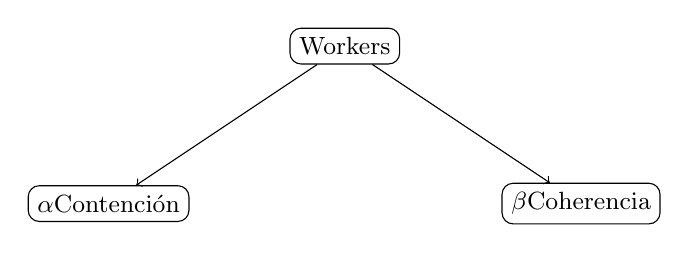
\begin{tikzpicture}[font=\small]
\node[draw, rounded corners] (workers) at (0,0) {Workers};

\node[draw, rounded corners] (alpha) at (-3,-2) {$\alpha$ \\ Contención};
\node[draw, rounded corners] (beta) at (3,-2) {$\beta$ \\ Coherencia};

\draw[->] (workers) -- (alpha);
\draw[->] (workers) -- (beta);
\end{tikzpicture}
\caption{Interpretación conceptual de los parámetros de la USL.}
\label{fig:usl_componentes}
\end{figure}

Obsérvese que cuando

\begin{equation}
\beta = 0,
\end{equation}

la expresión (\ref{eq:usl_appendix}) se reduce a una forma equivalente a la Ley de Amdahl.

La principal ventaja de la USL es que permite modelizar la denominada \emph{escalabilidad retrógrada}. En este fenómeno, el rendimiento aumenta inicialmente con el número de procesadores, alcanza un máximo y posteriormente disminuye debido a los costes crecientes de coordinación.

Esta situación no puede ser descrita por la formulación clásica de Amdahl.

\subsection{Extensión para SMT e Hyperthreading}

Las arquitecturas actuales incorporan mecanismos de \emph{Simultaneous Multithreading} (SMT), donde varios hilos lógicos comparten un mismo núcleo físico.

Sea:

\begin{itemize}
\item \(N\): número de núcleos físicos.
\item \(k\): número de hilos lanzados.
\item \(c\): eficiencia relativa de un hilo lógico cuando comparte núcleo.
\end{itemize}

Típicamente,

\begin{equation}
0.5 < c < 1.
\end{equation}

Mientras

\begin{equation}
k \leq N,
\end{equation}

cada hilo dispone de un núcleo físico dedicado y la escalabilidad sigue aproximadamente el comportamiento descrito por la USL.

Sin embargo, cuando

\begin{equation}
N < k \leq 2N,
\end{equation}

los nuevos hilos comienzan a compartir recursos internos del procesador, reduciendo la capacidad efectiva de cómputo.

Para representar este fenómeno se propone la siguiente generalización:

\begin{equation}
S(k)=
\begin{cases}
\dfrac{1}
{(1-P)+\dfrac{P}{k}+\beta(k-1)},
&
k\le N,
\\[1em]
\dfrac{1}
{(1-P)+\dfrac{P}{kc}+\beta(k-1)},
&
N<k\le2N.
\end{cases}
\label{eq:smt_model}
\end{equation}

La expresión anterior incorpora dos mecanismos distintos de degradación:

\begin{enumerate}
\item El término \(\beta(k-1)\), asociado a sincronización y coherencia.
\item El factor \(c\), asociado a la compartición de recursos físicos bajo SMT.
\end{enumerate}

Como consecuencia, el punto de saturación puede alcanzarse antes de lo previsto por la USL clásica y la región de escalabilidad retrógrada puede aparecer con un número menor de hilos.

\subsection{Interpretación para el motor Monte Carlo}

La simulación Monte Carlo constituye un caso particularmente favorable para la paralelización debido a que la generación de trayectorias es esencialmente independiente. Esto implica que la fracción paralelizable \(P\) es muy elevada.

No obstante, continúan existiendo componentes secuenciales asociadas a:

\begin{itemize}
\item Inicialización de la simulación.
\item Creación de tareas.
\item Agregación de resultados.
\item Ordenación de los valores de PnL para el cálculo de VaR y ES.
\end{itemize}

Asimismo, el acceso concurrente a memoria y el uso de hilos lógicos mediante SMT introducen efectos de contención que se vuelven más relevantes conforme aumenta el número de trabajadores.

Por este motivo, aunque la simulación Monte Carlo se aproxima al escenario ideal descrito por la Ley de Amdahl, la interpretación rigurosa de los resultados experimentales requiere considerar también los mecanismos descritos por la USL y su extensión para arquitecturas SMT.


\clearpage
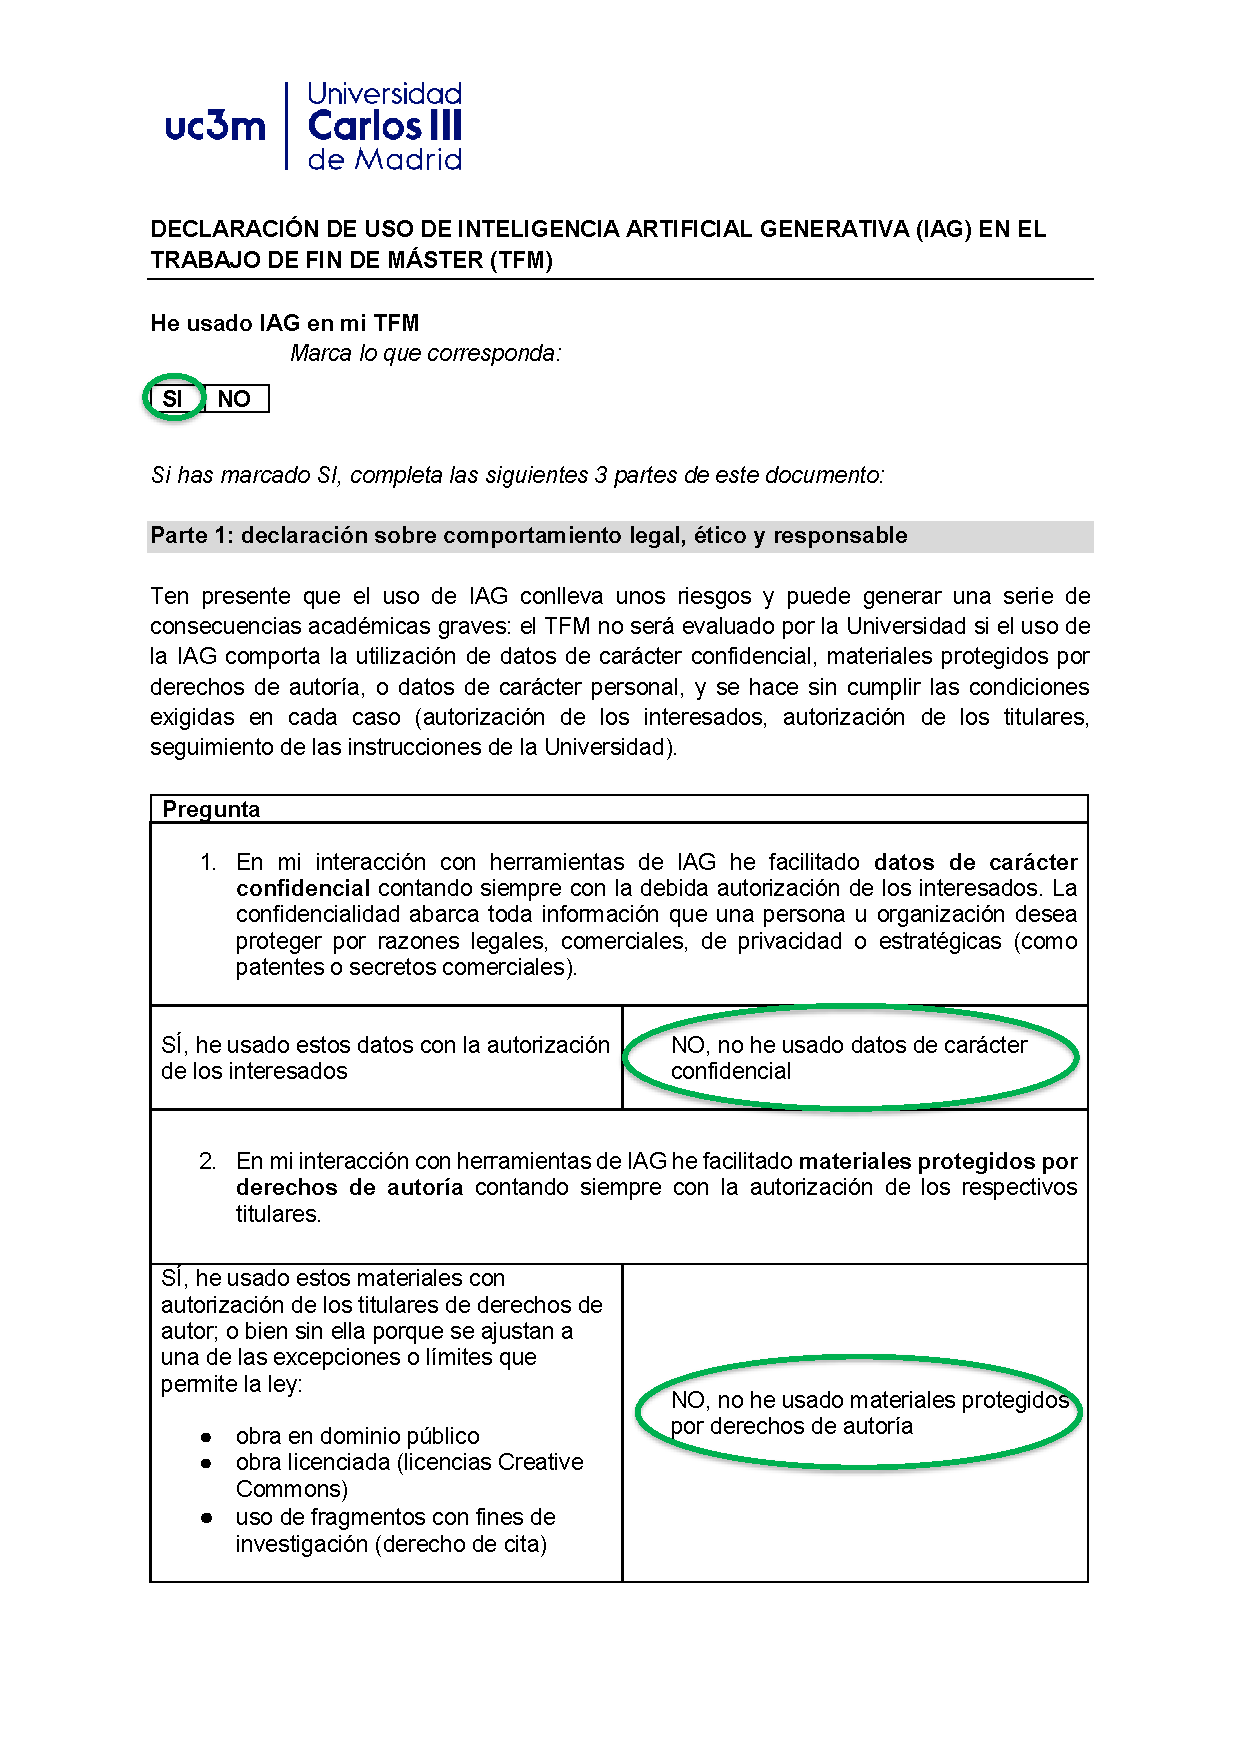
\includepdf[pages=-]{TFM_declaracion_uso_IAG_es_2026.pdf}
\end{document}
